% !TEX program = xelatex
\documentclass[12pt,a4paper,oneside]{report}
\usepackage{fontspec}
%\setmainfont{Arial}
\usepackage[english]{babel}
\usepackage{graphicx}
\usepackage[margin=3cm]{geometry}
\usepackage{setspace}
\usepackage{titlesec}
\usepackage{fancyhdr}
\usepackage{siunitx}
\usepackage{amsmath}
\usepackage{hyperref}
\usepackage{caption}
\usepackage{amssymb}

% Testina
\pagestyle{fancy}
\fancyhf{} % Cancella le impostazioni di default (es. numero in basso al centro)
\renewcommand{\sectionmark}[1]{\markright{\thesection\quad #1}}
\lhead{\normalfont\fontsize{10}{12}\selectfont\rightmark} 
\rhead{\normalfont\fontsize{10}{12}\selectfont\thepage}
\renewcommand{\headrulewidth}{0.4pt}
\renewcommand{\footrulewidth}{0pt}
\setlength{\headheight}{15pt} 

% Impagginamento
\onehalfspacing % Interlinea 1.5
\setlength{\parindent}{0.5cm} % Rientro della prima linea di 0.5 cm
\setlength{\parskip}{0pt} % Evita il salto di riga tra i paragrafi

% Chapter format
\titleformat{\chapter}[hang]
  {\normalfont\fontsize{14}{17}\bfseries}
  {\thechapter\quad}
  {0pt}
  {}
\titlespacing*{\chapter}{0pt}{-20pt}{20pt}

% Section format
\titleformat{\section}
  {\normalfont\fontsize{12}{15}\bfseries}
  {\thesection\quad}
  {0pt}
  {}
\titlespacing*{\section}{0pt}{15pt}{10pt}

% Subsection format
\titleformat{\subsection}
  {\normalfont\fontsize{12}{15}\bfseries}
  {\thesubsection\quad}
  {0pt}
  {}
\titlespacing*{\subsection}{0pt}{12pt}{8pt}

% Caption format
\captionsetup[figure]{
    font=footnotesize,
    labelfont=bf,
    labelsep=period,
    justification=justified,
    singlelinecheck=false % Prevents LaTeX from centering short single-line captions
}
\addto\captionsenglish{\renewcommand{\figurename}{Fig.}}

% Table format
\captionsetup[table]{
    font=footnotesize,
    labelfont=bf,
    labelsep=period,
    justification=justified,
    singlelinecheck=false % Prevents LaTeX from centering short single-line captions
}
\addto\captionsenglish{\renewcommand{\tablename}{Table}}
\renewcommand{\arraystretch}{1.3} % Per aumentare l'interlinea nella tabella

\begin{document}

\begin{titlepage}
    
    \centering
    \pagestyle{empty} % no page number on this page
    
    \begin{spacing}{1.0}
        
\includegraphics[width=0.9\textwidth]{tesiSCIENZE_TECNOLOGIE.jpg} 
    \end{spacing}
    
    \vspace{2.5cm} 
    
    {\LARGE Corso di Laurea Triennale in Fisica \\}
    
    \vfill 
    
    {\LARGE\bfseries The impact of redshift measurement errors in Euclid surveys on projected clustering statistics \\}
    
    \vfill 
    
    \noindent
    \begin{flushleft}
        {\large\textbf{Relatore:}}\\
        {\large Prof. Luigi Guzzo}\\[0.4cm]
        {\large\textbf{Correlatore:}}\\
        {\large Dott. Martin Kärcher}
    \end{flushleft}
    \begin{flushright}
        {\large\textbf{Elaborato di Tesi di:}}\\
        {\large Andrea Inveninato}\\
        {\large Matricola 11494A}
    \end{flushright}
    
    \vfill
    
    {\large A.A. 2025--2026}

\end{titlepage}

\pagenumbering{roman}

% abstract
\chapter*{Abstract}\label{chap:Abstract}
\addcontentsline{toc}{chapter}{Abstract}
In the thesis, simulated samples from the \textit{Euclid} spectroscopic survey will be analyzed, which reproduce different levels of contamination from spurious measurements in the redshift catalog produced by the satellite. The aim is to verify whether their impact on clustering estimates and the resulting cosmological analysis can be mitigated by adopting projected statistics, in which the effect is integrated and possibly marginalized.
\newpage

% index
\tableofcontents
\newpage


\chapter*{Introduction}\label{chap:Introduction}
\addcontentsline{toc}{chapter}{Introduction}
The distribution of galaxies on a large scale represents one of the most powerful tools for probing the structure of the Universe and acquiring information about the fundamental parameters that govern cosmic evolution. Over the past twenty-five years, the $\Lambda$ Cold Dark Matter ($\Lambda \mathrm{CDM}$) model has established itself as the standard model for describing the dynamics and composition of the Universe. In this model, the Universe is composed of approximately $68\%$ dark energy, $27\%$ dark matter and only the remaining $5\%$ as ordinary baryonic matter. While the $\Lambda \mathrm{CDM}$ model provides an extremely effective description of the observed distribution of large-scale structures, the fundamental nature of these dark components remains, to this day, one of the greatest mysteries in cosmology, and more refined and precise measurements could help us uncover their true nature.

In this context, the European Space Agency's \textit{Euclid} mission was conceived and successfully launched in 2023. \textit{Euclid} will collect an unprecedented dataset, observing nearly one third of the entire sky, and will use two main probes to constrain cosmological parameters: galaxy clustering and weak lensing. The ultimate aim is to create one of the largest most detailed three-dimensional maps of the Universe and investigate the true nature of the dark components.

On the other hand, because we observe the Universe from a single vantage point, we cannot directly measure three-dimensional spatial coordinates. Instead, we rely on the cosmological redshift $z$ as a proxy to radial distances. To achieve this, the \textit{Euclid} satellite uses slitless spectroscopy and the Near-Infrared Spectrometer and Photometer (NISP) to measure the position of the strongest emission lines in the galaxies' spectra, in particular the $\mathbf{H}\,\alpha$ line. By measuring the shift of spectral lines from distant galaxies, we can infer their radial distance from us, through the Hubble parameter.

However, this mapping assumes we are measuring the true cosmological redshift. In reality, galaxy surveys such as \textit{Euclid} determine redshifts spectroscopically by identifying specific emission lines. Therefore, systematic errors in the redshift determination can introduce contaminants in the spectroscopic sample and ultimately alter the observed galaxy spatial distribution. For instance, a more distant or closer galaxy emitting a stronger line that mimics the target $\mathbf{H}\,\alpha$ signal will be misidentified. These misidentified galaxies are known as \textit{interlopers}. When an interloper is included in the catalog, its incorrect redshift assigns it to a completely wrong spatial distance. This can affect the clustering statistics and in turn the cosmological parameters obtained from them.

The purpose of this project is to analyse realistic types and fractions of redshift interlopers. In order to do so, we study a suite of $1000$ mock catalogues, named \textit{EuclidLargeMocks} (ELM), published by the Euclid Consortium. We use this suite for our analysis as it accurately replicates the interloper population and proportions anticipated in the Euclid Wide Survey (EWS). By testing both standard clustering statistics and projected statistics, we aim to evaluate to which extent the impact of these spurious measurements on cosmological parameters can be successfully mitigated.
\newpage

\pagenumbering{arabic}
\chapter{Cosmology}\label{chap:Cosmology}
Cosmology is the scientific study of the Universe as a whole: its origin, evolution, large-scale structure, and ultimate fate. While the study of cosmic structures historically relied on qualitative theories, modern cosmology is a rigorous, data-driven branch of physics. It combines large-scale astronomical observations with advanced statistical methods and theoretical models to map the history of our universe over billions of years.

This modern mathematical description of the Universe has his roots in Albert Einstein's General Theory of Relativity (1915), which replaced Newtonian gravity with the geometric curvature of spacetime, thereby providing the essential theoretical foundation required to construct self-consistent cosmic models. The first observations began in 1929, when Edwin Hubble discovered a linear relationship between a galaxy's distance and its recessional velocity, providing the first strong observational evidence that the Universe is not static, but expanding.

Built on the concept of an expanding cosmos, the first step towards the modern cosmological model was made: astronomers suggested that the Universe evolved from a very hot, dense state where matter and radiation were in thermal equilibrium. It was indeed found, in 1964, the trace of this early phase of the universe with the detection of the Cosmic Microwave Background Radiation (CMB). As structural modeling advanced in the early 1980s, the gravitational pull of visible baryonic matter proved mathematically insufficient to explain the formation of large-scale cosmic structure or observed galactic rotation curves. To resolve this discrepancy, (Cold) Dark Matter was introduced as a non-baryonic component that accounts for nearly $\SI{27}{\%}$ of the Universe.

In the late 1990s, however, cosmology faced another major turning point, when observations of distant Type Ia supernovae - powerful and luminous explosions of stars that serve as cosmic “standard candles” due to their uniform intrinsic luminosity - revealed that the expansion of the Universe is not slowing down under the attractive influence of gravity, but is instead accelerating. This unexpected acceleration implied the existence of a dominant component that acts like a repulsive force. Interpreted most simply as a Cosmological Constant ($\Lambda$) in Einstein's field equations, this component became known as Dark Energy. The resulting $\Lambda \mathrm{CDM}$ model successfully integrated these discoveries into a standard model of cosmology, describing a spatially flat universe composed of approximately $\SI{5}{\%}$ ordinary baryonic matter, $\SI{27}{\%}$ Dark Matter, and $\SI{68}{\%}$ Dark Energy.

I used \cite{Longair} as a main reference to write the following sections of this chapter.

\section{The FLRW Metric}\label{sec:FLRW_Metric}
The standard cosmological model is built upon Einstein's General Theory of Relativity, according to which the distribution of mass and energy determines the curvature of spacetime. This curvature, in turn, determines the motion of matter and radiation. Einstein's field equations thus establish a dynamic relationship between geometry and energy content, making it possible to derive a metric, that is, a definition of the distance between two events in spacetime. To achieve this, we must apply the \textit{Cosmological Principle}, which postulates that, on sufficiently large scales, the Universe is both homogeneous (invariant under spatial translation) and isotropic (invariant under spatial rotation). In differential geometry, the most general spacetime metric that satisfies these strict symmetry requirements is the \textit{Friedmann-Lemaître-Robertson-Walker} (FLRW) metric:
\begin{equation}
  \mathrm{d}s^2 = -c^2\mathrm{d}t^2 + a^2(t)\left[ \frac{\mathrm{d}r^2}{1 - k r^2} + r^2 \left( \mathrm{d}\theta^2 + \sin^2{\theta} \mathrm{d}\varphi \right) \right] \; ,
  \label{eq:FLRW_Metric}
\end{equation}
where $t$ represents the cosmic time, which is the proper time measured by a comoving observer (an observer at rest relative to the local cosmic expansion) and $(r,\varphi,\theta)$ are the comoving coordinates, which remain constant for objects moving solely due to the cosmic expansion, meaning any localized peculiar velocities are ignored. In addition, $a(t)$ is the dimensionless scale factor, a time-dependent function that parameterizes the expansion of the Universe. By convention, it is normalized to unity at the present epoch $t_0$, that is, $a(t_0) = 1$. The paramater $k$ is the spatial curvature parameter \cite{CurvatureScalar}, a constant that determines the global geometry of the spatial hypersurfaces, and can take three discrete values:
\[
k =
\begin{cases}
  -1: & \text{negative curvature (open, hyperbolic geometry)} \\
  0: & \text{zero curvature (flat, Euclidean geometry)} \\
  +1: & \text{positive curvature (closed, spherical geometry)}
\end{cases}\label{eq:k_param} \; .
\]
In the case of $\Lambda\mathrm{CDM}$ model, the universe is geometrically flat ($k = 0$).

\section{Friedman's Equations}\label{sec:Friedman's_Equations}
While the FLRW metric describes the geometry of a homogeneous and isotropic universe, it does not dictate how the scale factor $a(t)$ evolves over time. To determine the dynamics of cosmic expansion, we must solve the \textit{Einstein Field Equations} (EFE):
\begin{equation}
  R_{\mu \nu} - \frac{1}{2}g_{\mu \nu}R + \Lambda g_{\mu \nu} = \frac{8 \pi G}{c^4} T_{\mu \nu} \; ,
  \label{eq:EFE}
\end{equation}
where $R_{\mu \nu}$ and $R$ are respectively the Ricci tensor and scalar, the latter also known as scalar curvature, $g_{\mu \nu}$ is the metric tensor and $\Lambda$ is the cosmological constant; $G$ and $c$ are respectively the gravitational constant and the speed of light, while $T_{\mu \nu}$ is the stress-energy tensor, which describes the density and flux of energy and momentum in spacetime.

By modeling the matter and energy content of the Universe as a perfect fluid, its energy-momentum tensor can be written in its rest frame as $T^\mu_\nu = \text{diag}(-\rho c^2, p, p, p)$, where $\rho(t)$ is the total energy density and $p(t)$ is the isotropic pressure. Inserting this tensor and the FLRW metric into the EFE yields the two \textit{Friedman Equations}, which govern the evolution of the scale factor:
\begin{equation}
  \left(\frac{\dot{a}}{a}\right)^2 = \frac{8 \pi G}{3}\rho - \frac{k c^2}{a^2} + \frac{\Lambda}{3}
  \label{eq:Friedmann_I}
\end{equation}
\begin{equation}
  \frac{\ddot{a}}{a} = -\frac{4 \pi G}{3} \left( \rho + \frac{3P}{c^2} \right) + \frac{\Lambda}{3}
  \label{eq:Friedmann_II}
\end{equation}
where the overdots represent derivatives with respect to cosmic time $t$.

These equations describe the evolution of the scale factor $a(t)$ of the universe as a function of the density $\rho$ and the pressure $P$ associated with all the energy components present, in this situation treated in the case of a perfect fluid. The components of the standard cosmological model, in terms of density $\rho$, are matter $(\rho_m)$, radiation $(\rho_r)$ and finally dark energy, whose equivalent vacuum energy density is defined as $\rho_\Lambda = \frac{\Lambda}{8 \pi G}$.

The energy density of each of these cosmic components possesses a specific mathematical dependence on the scale factor $a$, derived from the fluid conservation equation:%($\frac{\mathrm{d}\rho}{\mathrm{d}a} + \frac{3(\rho + P/c^2)}{a} = 0$):
\begin{itemize}
  \item $\rho \sim a^{-4} \, , \, P = \frac{1}{3}\rho \, ,$ in a Universe dominated by radiation;
  \item $\rho \sim a^{-3} \, , \, P = 0 \, ,$ in a Universe dominated by matter;
  \item $\rho = \mathrm{const} \, , \, P = -\rho \, ,$ in a Universe dominated by dark energy.
\end{itemize}
It is now convenient to introduce the \textit{critical density} $\rho_\mathrm{c}$, defined as the total density required today to obtain a perfectly flat universe ($k = 0$). Substituting this condition into the first Friedman equation, we obtain
\begin{equation}
  \rho_\mathrm{c} = \frac{3H^2}{8 \pi G} \; ,
  \label{eq:rho_crit}
\end{equation}
where we have defined the Hubble parameter as $H := \frac{\dot{a}}{a}$. When evaluated today, this is commonly referred to as the Hubble constant, $H_0 \approx 70 \, \mathrm{km \, s^{-1} \, Mpc^{-1}}$. To express cosmological distances, $t$ is traditional to use a dimensionless scaling factor $h$, i.e. $h := \frac{H_0}{100 \, \mathrm{km \, s^{-1} \, Mpc^{-1}}}$. At this point, it is convenient to express the densities $\rho_i$ of each component in terms of the critical density $\rho_\mathrm{c}$, that is using the fractional densities $\Omega_i := \frac{\rho_i}{\rho_\mathrm{c}}$. In this way, the first Friedman equation can be rewritten to show the evolution of the expansion rate across time
\begin{equation}
  H^2(a) = H_0^2 \left( \Omega_{m,0} \, a^{-3} + \Omega_{r,0} \, a^{-4} + \Omega_{k,0} \, a^{-2} + \Omega_{\Lambda,0} \right) \; ,
  \label{eq:Ha}
\end{equation}
where the subscript $0$ indicates that the parameter is evaluated at the present time. Usually, the density parameter $\Omega_{r,0}$ associated with radiation is neglected in the late-time Universe, as its value today is remarkably small ($\Omega_{r,0} \sim 10^{-4}$). It is now clear that the expansion rate of the Universe depends explicitly on the composition of mass-energy within the Universe itself. Since we assumed a spatially flat universe ($\Omega_{k,0} = 0$) as in the standard $\Lambda \mathrm{CDM}$ model, the density parameters of the remaining components add up to $1$.

\section{Cosmological Redshift}\label{sec:CosmologicalRedshift}
When observing the sky, it is not possible to measure the scale factor $a(t)$ directly. In galaxy surveys, the actual observable is the \textit{cosmological redshift} ($z$), which represents the observed shift of a source's spectrum towards longer wavelengths and is defined as
\begin{equation}
  z = \frac{\lambda_\mathrm{obs} - \lambda_\mathrm{rest}}{\lambda_\mathrm{obs}} \; ,
  \label{eq:Redshift_def}
\end{equation}
where $\lambda_\mathrm{obs}$ is the observed wavelength, while $\lambda_\mathrm{rest}$ is the wavelength as emitted by the source. 

Intuitively, redshift can be interpreted as a measure of the Newtonian Doppler shift generated by the recessional velocity of galaxies due to the Universe’s expansion. At low redshift ($z \ll 1$), this interpretation holds true and was indeed the one used by Hubble to derive his previously mentioned velocity-distance relationship $v = H_0 \, r$.

On cosmological scales, however, redshift takes on a far deeper meaning as it serves as direct metric of the expansion of spacetime itself. To derive this relationship between the scale factor and redshift, we consider the kinematics of electromagnetic radiation: a wave packet of frequency $\nu_1$, emitted between cosmic times $t_1$ and $t_1 + \Delta t_1$ from a distant object, is received by an observer at the present epoch between cosmic times $t_0$ and $t_0 + \Delta t_0$. Since photons travel along null geodesics ($\mathrm{d} s^2 = 0 $), the FLRW metric simplifies to:
\begin{equation}
  0 = -c^2 \mathrm{d} t^2 + a^2(t) \mathrm{d} r^2 \; ,
  \label{eq:NullGeodesics}
\end{equation}
where only radial propagation has been taken into account due to spherical symmetry ($\mathrm{d}\theta = \mathrm{d}\varphi = 0$). Rearranging this expression we obtain
\begin{equation}
  \mathrm{d} r = \pm \frac{c \, \mathrm{d} t}{a(t)} \; .
  \label{eq:NullGeodesics_2}
\end{equation}
As the radial distance decreases with time in an observer-centered frame, we can select the negative solution without any loss of generality.

Let the first wave crest be emitted at cosmic time $t_1$ and observed at the origin at time $t_0$. The next wave crest is emitted a single period later at $t_1 + \Delta t_1$ and observed at $t_0 + \Delta t_0$. Integrating Eq. \eqref{eq:NullGeodesics_2} for both wave edges of the wave packet yields:
\begin{equation}
  \int_{t_1}^{t_0} \frac{c \, \mathrm{d}t}{a(t)} = - \int_{r}^{0} dr \; \text{;} \quad \int_{t_1 + \Delta t_1}^{t_0 + \Delta t_0} \frac{c \, \mathrm{d}t}{a(t)} = - \int_{r}^{0} dr \; .
  \label{eq:WavePackets}
\end{equation}
Since both edges must travel the same comoving distance, which remains constant over time, it follows that
\begin{equation}
  \int_{t_1}^{t_0} \frac{c \, \mathrm{d}t}{a(t)} = \int_{t_1 + \Delta t_1}^{t_0 + \Delta t_0} \frac{c \, \mathrm{d}t}{a(t)} \quad .
  \label{eq:WavePackets_Equality}
\end{equation}
Given that $a(t_0) = 1$ and assuming $\Delta t_0$ and $\Delta t_1$ to be small enough to approximate $a(t)$ as constant over these
intervals, the relation simplifies directly to:
\begin{equation}
  \Delta t_0 = \frac{\Delta t_1}{a(t_1)} \; ;
  \label{eq:TimeDilation}
\end{equation}
this equation represents the cosmological time dilation.

Knowing that $\Delta t_i = \frac{1}{\nu_i}$, we obtain the fundamental relation between redshift and cosmic expansion:
\begin{equation}
  z = \frac{\lambda_\mathrm{obs} - \lambda_\mathrm{rest}}{\lambda_\mathrm{obs}} = \frac{\nu_1}{\nu_0} - 1 = \frac{1}{a(t_1)} - 1 \; ,
  \label{eq:Redshift_Equality}
\end{equation}
which can be rewritten as
\begin{equation}
  a(t_1) = \frac{1}{1 + z} \; .
  \label{eq:ScaleFactor_Redshift}
\end{equation}

As a result, redshift provides a direct measurement of the scale factor of the Universe at the moment of emission. For instance, observing a galaxy at redshift $z = 1$ implies the scale factor of the universe when the radiation was emitted was $a(t) = 0.5$, meaning that at that time the proper distances between galaxies were half their present value.

By utilizing the coordinate transformation $a = (1 + z)^{-1}$, we can transition our theoretical framework from the unobservable scale factor to the directly measurable redshift. Rewriting the Hubble parameter expansion Eq. \eqref{eq:Ha}, while neglecting the contributions from radiation and curvature, yields the $\Lambda \mathrm{CDM}$ expansion rate as a function of redshift:
\begin{equation}
  H(z) = H_0 \sqrt{\Omega_{m,0} \, (1 + z)^3 + \Omega_{\Lambda,0}} \; .
  \label{eq:HubbleParameter}
\end{equation}
This equation is crucial for cosmology. It establishes a direct connection between the theoretically obtained equation for the expansion rate of the Universe, $H(z)$, and measurable data.

\section{Comoving Distance}\label{sec:Comoving_Distance}
With the expansion rate $H(z)$ explicitly defined as a function of the observational redshift, we can compute the fundamental distance used to map the large-scale structure: the \textit{comoving distance} ($D_\mathrm{c}$). The comoving distance factors out the universal expansion, ensuring that two objects at fixed cosmic coordinates maintain a constant distance over time.

By revisiting the radial null geodesic condition ($\mathrm{d} s^2 = 0$) given in Eq. \eqref{eq:NullGeodesics_2}, the comoving distance traveled by light from a galaxy at redshift $z$ to an observer at $z=0$ is given by the spatial integral of $\mathrm{d} r$
\begin{equation}
  D_{\mathrm{c}}(t) = \int_{t}^{t_0} \frac{c \, \mathrm{d} t'}{a(t')} = \int_{a}^{1} \frac{c \, \mathrm{d} a'}{a'^2 H(a')} = \int_{0}^{z} \frac{c \, \mathrm{d} z'}{H(z')} \; .
  \label{eq:ComovingDistance}
\end{equation}
In the local Universe limit where $z \ll 1$, this relation reduces to $r \sim \frac{c z}{H_0}$, which recovers the empirical velocity-distance law found by Hubble.

\section{Large-Scale Structure Statistics}\label{sec:LSStructureStatistics}
Our description of the Universe, so far, has relied entirely on the assumptions of a perfectly homogeneous and isotropic Universe. While this ideal model accurately describes the global expansion history of the cosmos on its largest scales, the real Universe on smaller scales is highly inhomogeneous, ranging from isolated objects, through groups and clusters of galaxies to superclusters and giant voids in their distribution.

Since we cannot model the precise position of every individual galaxy, we must treat the Universe as a stochastic random field. To quantify these structures, we define the dimensionless \textit{density contrast} field, $\delta(\mathbf{x})$, which measures the local deviation of matter density $\rho(\mathbf{x})$ at a spatial position $\mathbf{x}$ from the global mean density of the Universe $\bar{\rho}$:
\begin{equation}
  \delta(\mathbf{x}) \equiv \frac{\rho(\mathbf{x}) - \bar{\rho}}{\bar{\rho}} \; .
  \label{eq:DensityContrast}
\end{equation}
By definition, regions where $\delta > 0$ represent overdensities (such as galaxy clusters), while regions where $\delta < 0$ correspond to underdensities (voids).

\subsection{Two-Point Correlation Functions}\label{subsec:2PCF}
To extract cosmological information from the inhomogeneous distribution of galaxies, we make use of statistical methods, in particular the \textit{Two-Point Correlation Functions} (2PCF)~\cite{TwoPCF}. The spatial two-point correlation function $\xi (\mathbf{r})$ describes the excess probability of finding a galaxy at distance $\mathbf{r}$ from a galaxy selected randomly over that expected in a uniform, Poisson distribution. It is implicitly defined by the relation
\begin{equation}
  \mathrm{d} N (\mathbf{r}) = N_0 \left[ 1 + \xi (\mathbf{r}) \right] \mathrm{d} V \; ,
  \label{eq:2PCF}
\end{equation}
where $\mathrm{d} N (\mathbf{r})$ represents the number of galaxies in the volume $\mathrm{d} V$ at a distance $\mathbf{r}$ from the selected galaxy and $N_0$ is a suitably-defined average background number density of galaxies. The 2PCF can be directly related to the density contrast:
\begin{equation}
  \xi (\mathbf{r}) = \langle \delta (\mathbf{x}) \, \delta (\mathbf{x} + \mathbf{r}) \rangle \; ,
  \label{eq:2PCF_DensityContrast}
\end{equation}
where the angle brackets $\langle \, \dots \rangle$ denote an ensemble average over all spatial positions $\mathbf{x}$. Under the assumption of ergodicity, this ensemble average can be evaluated as a spatial average over a sufficiently large volume of the Universe.

In practical applications with actual galaxy catalogs, $\xi(\mathbf{r})$ cannot be calculated via continuous integrals. The standard method used to evaluate the 2PCF is the \textit{Landy-Szalay} (LS) estimator~\cite{LSEstimator}. It is obtained, first of all, by determining a catalogue overdensity, defined as the fractional difference between the data and random counts in the catalog. By counting pairs of galaxies within a given survey volume and comparing them to an artificial catalog of randomly distributed points occupying the exact same geometric volume, the overdensity in galaxy counts at any position $\mathbf{x}$ is
\begin{equation}
  \delta (\mathbf{x}) = \frac{D(\mathbf{x}) - R(\mathbf{x})}{R(\mathbf{x})} \; ,
  \label{eq:LS_DensityContrast}
\end{equation}
where $D(\mathbf{x})$ and $R(\mathbf{x})$ are data and random catalogue counts at position $\mathbf{x}$. 
The Landy-Szalay estimator is, thereby, computed by taking the auto-correlation of the overdensity, as in Eq. \eqref{eq:2PCF_DensityContrast}:
\begin{equation}
  \xi (\mathbf{r}) = \frac{\mathrm{DD}(\mathbf{r}) - 2\mathrm{DR}(\mathbf{r}) + \mathrm{RR}(\mathbf{r})}{\mathrm{RR}(\mathbf{r})} \; , 
  \label{eq:LSEstimator}
\end{equation}
where $\mathrm{DD}(\mathbf{r})$, $\mathrm{DR}(\mathbf{r})$, $\mathrm{RR}(\mathbf{r})$ are respectively the normalized data-data, data-random and random-random pair counts as a function of the pair separation vector $\mathbf{r}$. The normalisation of pair counts originates from the fact that the random catalogue contains a much larger number of objects than the data catalogue, such that
\begin{equation}
  \mathrm{DD}(\mathbf{r}) = \frac{2 \widehat{\mathrm{DD}}(\mathbf{r})}{N_\mathrm{D} (N_\mathrm{D}-1)} \; ,
  \label{eq:DD}
\end{equation}
\begin{equation}
  \mathrm{DR}(\mathbf{r}) = \frac{\widehat{\mathrm{DR}}(\mathbf{r})}{N_\mathrm{D} N_\mathrm{R}} \; ,
  \label{eq:DR}
\end{equation}
\begin{equation}
  \mathrm{RR}(\mathbf{r}) = \frac{2 \widehat{\mathrm{RR}}(\mathbf{r})}{N_\mathrm{R} (N_\mathrm{R}-1)} \; ,
  \label{eq:RR}
\end{equation}
where $\widehat{\mathrm{DD}}(\mathbf{r})$, $\widehat{\mathrm{DR}}(\mathbf{r})$, $\widehat{\mathrm{RR}}(\mathbf{r})$ are raw counts, and $N_\mathrm{D}$ and $N_\mathrm{R}$ are the total number of objects in the data and random catalogues respectively.

\subsection{Redshift-Space Distortions}\label{subsec:RedshiftSpaceDistortions}
In an ideal scenario, the distance between two galaxies would be purely geometrically determined and the 2PCF would depend solely on the separation modulus $\xi (r)$. However, in the observed world the distance is altered as the total observed redshift of a galaxy is a combination of two distinct physical components: the global cosmological expansion of the Universe (Hubble recession) and the localized, gravitationally induced motion of the galaxy relative to that flow, known as its peculiar velocity ($v_{\mathrm{pec}}$). Therefore, the observed redshift is computed as follows:
\begin{equation}
  z_\mathrm{obs} = z_\mathrm{c} + \frac{v_\parallel}{c} (1 + z_\mathrm{c}) \; ,
  \label{eq:z_obs}
\end{equation}
where $z_\mathrm{c}$ is the cosmological redshift due to the Hubble recession velocity at the comoving distance of the object and $v_\parallel$ is the line-of-sight component of its centre of mass velocity. Although these shifts are small compared to the true distance $r(z_\mathrm{c})$ (less than $\SI{1}{\percent}$ at $z \sim 0.3$), they strongly affect clustering measurements which depend on separations between galaxies.

Because peculiar velocities only shift galaxies along the line-of-sight, they introduce systematic distortions in our spatial map. This phenomenon, known as \textit{Redshift-Space Distortions} (RSD)~\cite{RedshiftSpace}, breaks the intrinsic spherical symmetry of the two-point correlation function, turning $\xi(\mathbf{r})$ anisotropic. As a result, the separation vector $\mathbf{r}$ between a pair of galaxies is decomposed into two orthogonal components relative to the line-of-sight: the perpendicular separation ($r_\mathrm{p}$), which is immune to RSD, and the parallel, along the line-of-sight, separation ($\pi$), which contains all the redshift-space distortions:
\begin{equation}
  \pi = \frac{\mathbf{r} \cdot \mathbf{d}}{|\mathbf{d}|} \; , \quad r_\mathrm{p} = \sqrt{|\mathbf{r}|^2 - \pi^2} \; ,
  \label{eq:rp_pi}
\end{equation}
where $\mathbf{r}$ is the separation vector between the two galaxies and $\mathbf{d}$ is the line-of-sight vector pointing to the midpoint of the galaxy pair. The resulting 2PCF is denoted as $\xi(r_\mathrm{p}, \pi)$.

Alternatively, the separation can be expressed in spherical coordinates via the scalar distance $s = \sqrt{r_\mathrm{p}^2 + \pi^2}$ and the directional parameter $\mu \equiv \cos\theta = \frac{\pi}{s}$, where $\theta$ is the angle between the separation vector and the line-of-sight. This allows the anisotropic correlation function to be written as $\xi(\mu, s)$.

\subsection{Clustering statistics}\label{subsec:ClusteringStatistics}
To extract cosmological constraints from anisotropic clustering, the standard practice is to project or integrate the 2D correlation function over specific angular or spatial intervals~\cite{Kazin}. Depending on the goal, three main monodimensional observables are utilized.

\paragraph{Multipoles expansion}\label{parag:MultipolesExpansion}
The most common technique to compress the angular dependence of $\xi(s, \mu)$  is to expand the function into a series of Legendre polynomials, $\mathcal{P}_\ell(\mu)$. Using spherical harmonics, the anisotropic $\xi(\mu, s)$ may be written as
\begin{equation}
  \xi (\mu, s) = \sum_{\mathrm{even } \ell} \mathcal{P}_\ell (\mu) \xi_\ell(s) \; ,
  \label{eq:MultipolesExpansion}
\end{equation}
where $\mathcal{P}_\ell$ are Legendre polynomials [e.g. $\mathcal{P}_0 = 1$, $\mathcal{P}_2 = \frac{1}{2} (3\mu^2 -1)$, $\mathcal{P}_4 = \frac{1}{8} (35\mu^4 - 30\mu^2 + 3)$] and the multipole projections are defined as
\begin{equation}
  \xi_\ell \equiv \frac{2\ell + 1}{2} \int_{-1}^{1} \mathcal{P}_\ell (\mu) \xi(\mu,s) \mathrm{d}\mu \; .
  \label{eq:Multipoles}
\end{equation}
Note that, due to the symmetry of the FLRW metric and the nature of linear RSD, all odd multipoles ($\ell = 1, 3, \dots$) vanish.

\paragraph{Clustering wedges}\label{parag:ClusteringWedges}
An alternative compression method that does not depend on the mathematical assumptions of orthogonal polynomials is the calculation of clustering wedges, $\xi(\Delta\mu, s)$. Instead of integrating over the entire smooth distribution of $\mu$, the angular parameter space is divided into wide, discrete intervals
\begin{equation}
  \xi(\Delta\mu, s) \equiv \frac{\int_{\mu_\mathrm{min}}^{\mu_\mathrm{max}} \xi(\mu',s) \mathrm{d}\mu'}{\int_{\mu_\mathrm{min}}^{\mu_\mathrm{max}} \mathrm{d}\mu'} \; ,
  \label{eq:ClusteringWedges}
\end{equation}
where we assume the plane-parallel, or small angle, approximation, according to which two galaxies at the same distance from the observer yield $\mu = 0$ regardless of their angular distance.

Typically, the data is split into two halves: a transverse wedge $\xi_\perp(s)$ for $\mu \in [0, 0.5]$, which isolates galaxy pairs oriented perpendicular to the line-of-sight and is to a minimal extent impacted by redshift errors, and a radial wedge $\xi_\parallel(s)$ for $\mu \in [0.5, 1.0]$, which isolates pairs oriented along the line-of-sight, maximizing sensitivity to cosmic expansion and velocity effects.

\paragraph{Projected funcion}\label{parag:ProjectedFuncion}
To entirely eliminate the line-of-sight vulnerabilities, one can define the projected correlation function, $w_\mathrm{p}(r_\mathrm{p})$,  constructed by integrating $\xi(r_p, \pi)$ along the entire parallel separation axis:
\begin{equation}
  w_\mathrm{p}(r_\mathrm{p}) \equiv 2 \int_{0}^{\infty} \xi(r_\mathrm{p}, \pi) \mathrm{d} \pi \; .
  \label{eq:ProjectedFuncion}
\end{equation}

\chapter{Euclid}\label{chap:Euclid}
Launched in July 2023, \textit{Euclid} is a medium-class space telescope in the Cosmic Vision 2015-2025 program of the European Space Agency (ESA)\~\cite{Euclid}. Covering a redshift range up to $z \sim 2$ and executing a wide-field survey across approximately $\SI{14000}{deg^2}$ of the extragalactic sky, the mission aims to understand the nature of dark energy, dark matter, and the validity of the $\Lambda\mathrm{CDM}$ on cosmological scales.

To achieve these objectives, \textit{Euclid} simultaneously uses two powerful and complementary cosmological probes: Weak Lensing (WL), which charts the distribution of dark and luminous matter by measuring the gravitational “shearing” of images of distant galaxies, and Galaxy Clustering (GC), which relies on the measurement of spectroscopic redshifts to map the three-dimensional matter distribution of the Universe.

\textit{Euclid} gathers these precise measurements using two sophisticated instruments. The first one is the VIS (Visual Imager), which records the precise shapes of galaxies to analyze weak gravitational lensing. The second one, NISP (Near-Infrared Spectrometer and Photometer), is designed to provide multi-band photometry for galaxies detected by the VIS while conducting slitless grism spectroscopy to probe how those galaxies cluster together.

The main objective of the \textit{Euclid} mission is to constrain dynamical dark energy models and evaluate modified gravity theories. Furthermore, it will refine constraints on extensions to the standard cosmological model. In particular, \textit{Euclid} aims to further improve our understanding of the Universe's initial conditions and, when integrated with Planck data, substantially increase the precision of constraints on the total mass of neutrinos. According to the official mission overview (Mellier et al. 2024), \textit{Euclid} achieves this by operating from a halo orbit around the second Sun-Earth Lagrangian point (L2), an environment that provides exceptional thermal stability and an unobstructed view of the cosmos away from the optical interference of the Earth, Moon, and Sun.

\section{Mission scope}\label{sec:MissionScope}
The primary survey strategy is divided into two main components:
\begin{itemize}
  \item \textbf{Euclid Wide Survey (EWS)}: The flagship component of the mission, covering $\sim \SI{14000}{deg^2}$ of the sky (roughly one-third of the entire celestial sphere). It targets regions of the sky with low zodiacal light and low galactic extinction to maximize the detection of faint, high-redshift galaxies.
  \item \textbf{Euclid Deep Survey (EDS)}: Covering approximately $\SI{40}{deg^2}$ spread across three specialized patches of the sky. This survey observes areas at a depth two magnitudes deeper than the Wide Survey, serving as a vital calibration tool to quantify selection effects and systematic uncertainties in the main catalog.
\end{itemize}
By observing millions of active, star-forming galaxies across these expansive fields, \textit{Euclid} effectively samples the density contrast field $\delta(\mathbf{x})$ defined in Section~\ref{sec:LSStructureStatistics}. To transform these raw observations into the 3D comoving coordinates required for our Landy-Szalay clustering calculations, \textit{Euclid} relies on a dual-instrument payload capable of capturing both high-resolution images and specialized near-infrared spectra.

\subsection{Cosmological probes}\label{subsec:CosmologicalProbes}
To extract maximum cosmological information from its surveys, \textit{Euclid} is uniquely designed to combine two independent yet highly complementary observational techniques.

\paragraph{Weak lensing}\label{parag:WeakLensing}
The phenomenon of gravitational lensing, predicted by Einstein’s theory of General Relativity, occurs when light from distant galaxies is bent as it passes through the curved spacetime near massive objects. In some cases, the bending of the light is so significant that multiple images of the galaxy are formed; this is typically called strong gravitational lensing. In other cases, the light bending is subtle, and the images of galaxies are distorted, stretched and magnified in small amounts; this is named weak gravitational lensing~\cite{WeakLensing}. This type of lensing is neither strong enough to produce multiple images nor detectable using an individual galaxy; instead, the tidal field of a gravitational lens induces a coherent alignment of galaxy images, which can be quantified through correlations in their shapes.

By combining this information with measurements of the redshift distribution of the sources, we can trace the evolution of the large-scale structure (LSS), thereby allowing us to probe the effects of dark energy. \textit{Euclid} will achieve this, by acquiring the shapes of approximately $1.5$ billion galaxies through VIS and measuring their photometric redshifts with NISP.

\paragraph{Galaxy clustering}\label{parag:GalaxyClustering}
This probe uses galaxies as discrete luminous tracers of the underlying, inhomogeneous dark matter distribution. By measuring the three-dimensional spatial coordinates of tens of millions of galaxies, GC allows us to compute the two-point clustering statistics. From these statistics, we extract two major cosmological features: Baryon Acoustic Oscillations (BAO), which serve as a standard ruler to chart the expansion history $H(z)$, and Redshift-Space Distortions (RSD), which track the growth rate of cosmic structure to test theories of modified gravity.
To achieve this, \textit{Euclid} will use NISP’s slitless spectroscopy to measure the redshift of nearly 100 million galaxies in the range $0.9 < z < 1.8$.

\subsection{Primary scientific goals}\label{subsec:PrimaryScientificGoals}
As already mentioned, the \textit{Euclid} mission primarily aims to constrain dynamical dark energy models and evaluate modified gravity theories.

\paragraph{Dark energy models}\label{parag:DarkEnergyModel}
In the standard $\Lambda\mathrm{CDM}$ model, the equation-of-state parameter $w$ relates the pressure $P$ and the energy density $\rho c^2$ of a substance as $P \equiv w \rho c^2$. In the case of a cosmological constant $\Lambda \neq 0$, or a non-zero vacuum energy density, we obtain $w = -1$.

Despite dark energy making up about $\SI{68}{\percent}$ of the present-day energy density, we are unsure whether it is an actually cosmological constant, a field that evolves dynamically, or reflects a more profound modification of the gravitation laws at cosmological scales. To distinguish between such models we can analyze the way the equation-of-state parameter $w(z)$ varies with redshift. We adopt the model
\begin{equation}
  w(z) = w_0 + w_a \frac{z}{1 + z} \; ,
  \label{eq:wParameter}
\end{equation}
where $w_0$ represents the present-day value of the equation of state, and $w_a$ quantifies the dependence of dark energy with redshift to the first order in $(1-a)$, where $a = \frac{1}{(1 + z)}$ is the scale factor. The standard case for the cosmological constant corresponds to that in which $w_0 = - 1 $ and $w_a = 0$, and every result that differs will hint in the direction of a non-constant dark energy.

By measuring the spatial distribution of galaxies over a vast redshift range, \textit{Euclid} aims to measure the dark energy Figure of Merit (FoM), a parameter that compares the performance of different surveys. It is defined as the inverse square root of the covariance matrix determinant for the dark energy parameters:
\begin{equation}
  \mathrm{FoM} = \frac{1}{\sqrt{\mathrm{det}(\mathrm{cov}(w_0,w_a))}} \; .
  \label{eq:DE_FoM}
\end{equation}

In this way, larger values of FoM imply more precise measurements of the properties of dark energy. \textit{Euclid} seeks to achieve a $\mathrm{FoM} > 400$ which would represent a major improvement to current FoM for dark energy.

\paragraph{Modified theories of gravity}\label{parag:ModifiedGravity}
An alternative explanation for cosmic acceleration is that General Relativity is incomplete on megaparsec scales, requiring a modification to the laws of gravity. Analogous to the use of the dark energy equation of state, the dimensionless linear growth rate $f_\mathrm{g}(z)$ depends on $\Omega_\mathrm{m}(z)$, the redshift-dependent ratio of matter density divided by the critical density, as
\begin{equation}
  f_\mathrm{g}(z) \simeq [\Omega_\mathrm{m}(z)]^{\gamma_\mathrm{g}} \; ,
  \label{eq:LinearGrowthRate}
\end{equation}
where $\gamma_\mathrm{g} = 0.55$ is the growth index for a flat $\Lambda\mathrm{CDM}$ universe.

Any measured deviation from this value would point out a breakdown of Einstein’s equations on large scales. By measuring Redshift-Space Distortions in the galaxy clustering statistics, \textit{Euclid} aims to evaluate $\gamma_\mathrm{g}$ with a precision better than $0.02$ (that is $\SI{68}{\percent}$ confidence), providing a definitive test of General Relativity on cosmological scales.

\section{Slitless Spectroscopy}\label{sec:SlitlessSpectroscopy}
Traditional spectrographs isolate individual target galaxies using physical masks with narrow slits or fiber-optic cables. Although this method provides sharp, isolated spectra, it requires prior knowledge of the galaxies’ positions and limits the number of objects that can be observed simultaneously in a single exposure. For this reason, \textit{Euclid} uses slitless spectroscopy: a technique that employs a “grism” (a combination of a prism and a grating) to produce a dispersed image of a field in the sky without the use of apertures. Unlike slit spectroscopy, it does not isolate objects within the field, thus yielding a two-dimensional spectrum that is a convolution of the object’s physical shape and its spectral properties. With this technique, all sources are captured simultaneously, resulting in spectral contamination due to source overlap being one of the main challenges. To address this issue, different dispersion angles are used to separate the spectra in orthogonal directions. Initially, \textit{Euclid} planned to use three red grisms with dispersion angles of $\SI{0}{\degree}$, $\SI{180}{\degree}$ and $\SI{270}{\degree}$; however, performance issues with the $\SI{270}{\degree}$ grism led to the adoption of an alternative method, in which the remaining two grisms were rotated by $\SI{4}{\degree}$, providing a total of four different dispersion directions.

In addition to spectral contamination, slitless spectroscopy faces other significant challenges, such as increased sky background noise, which reduces the signal-to-noise ratio (SNR). The dominant background source for \textit{Euclid} is zodiacal light, which peaks near the plane of the ecliptic. Hence, the target area must have minimal contamination from the Galaxy, Solar System objects, and the zodiacal background. The intersection of the avoided regions around the Galactic and ecliptic planes leaves four separate dark areas on the sky for the EWS, which we refer to as the Region of Interest (RoI), indicated by the blue lines in Fig.~\ref{fig:EuclidRoI}. These areas are adjusted in size to maximise the overlap with the ground-based surveys providing complementary data needed for correcting instrument image blur and photometric redshift estimation.

\begin{figure}[t]
    \centering
    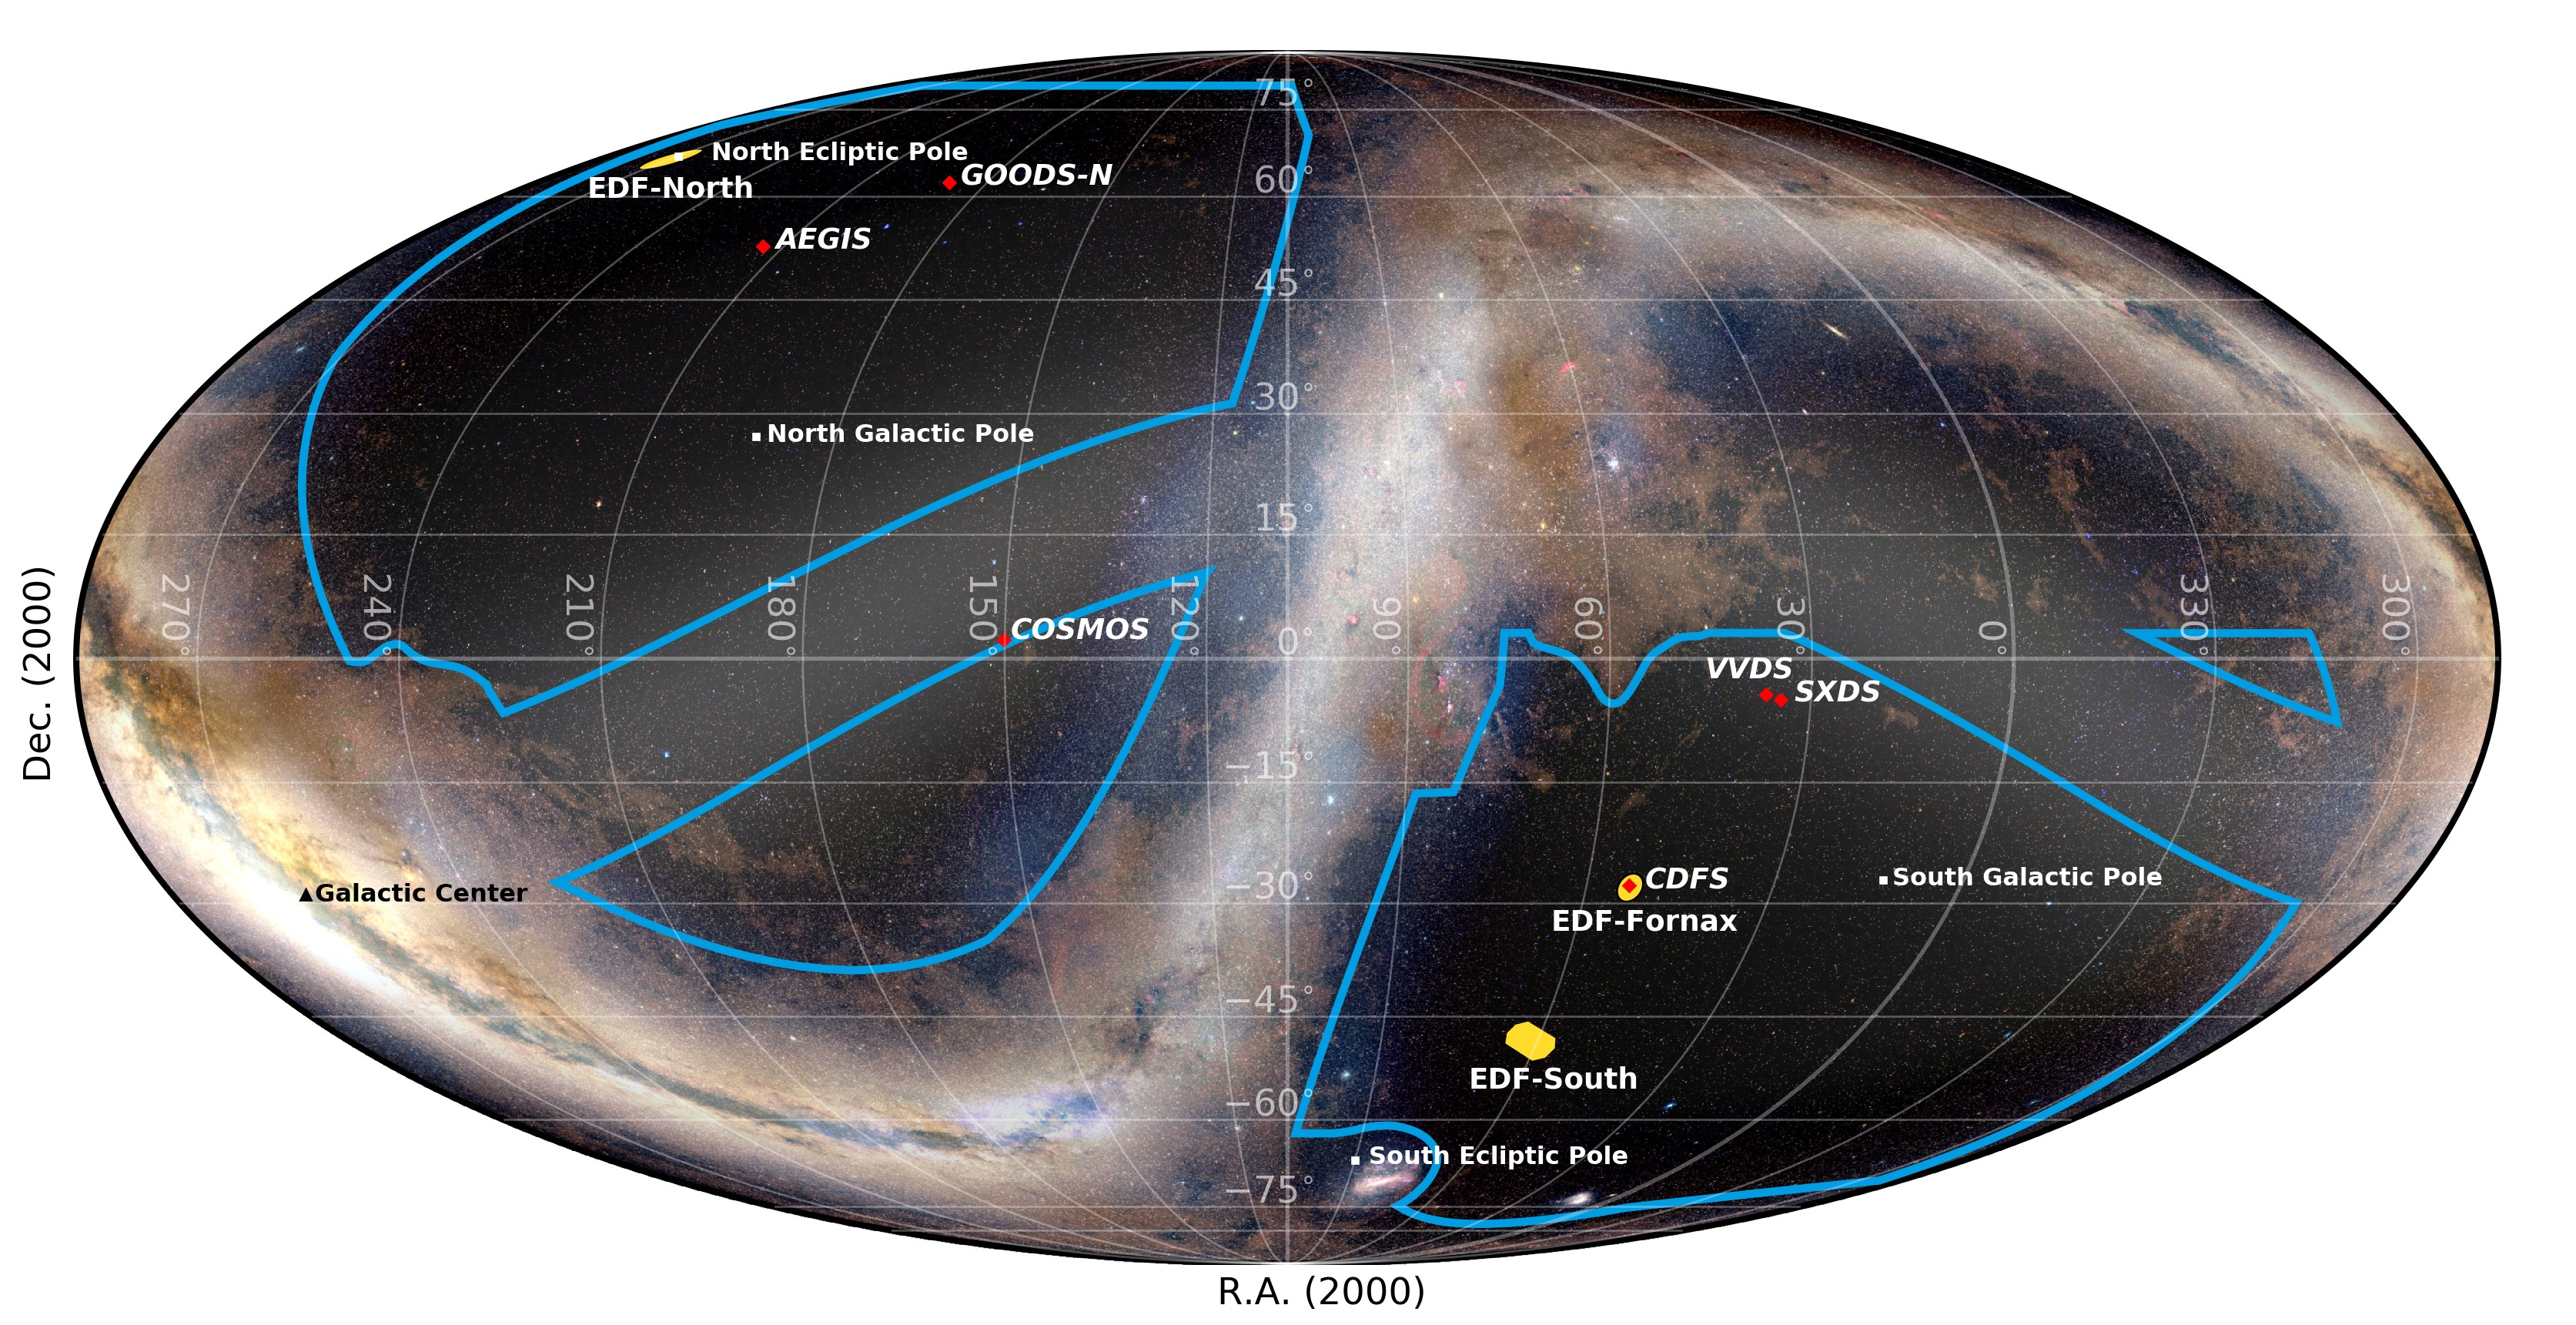
\includegraphics[width=\linewidth]{AllSkyEuclid.MollweideTrueSkyEWS.MOL.jpg}
    \caption{\textit{Euclid} region of interest (RoI) in an all-sky Mollweide projection. The blue borders enclose the $\SI{16000}{deg^2}$ RoI that contains the observed sky of the Euclid Wide Survey. The RoI excludes the Galactic and ecliptic planes. The triangular southern ‘island’ near $RA=\SI{330}{\degree}$ is restricted in size since the LSST does not extend to more northern latitudes. The Euclid Deep Fields are shown in yellow and the auxiliary fields with red marks (not to scale).}
    \label{fig:EuclidRoI}
\end{figure}

Nevertheless, slitless spectroscopy also offers several advantages, including a simpler instrument design, a wider field of view for the creation of extensive catalogues, and an efficient observational schedule.

\paragraph{The Near-Infrared Spectrometer and Photometer}\label{parag:NISP-S}
The spectroscopic channel of the Near-Infrared Spectrometer and Photometer (NISP-S) onboard \textit{Euclid} enables the simultaneous acquisition of thousands of slitless spectra across its field of view with uniform quality. The grism wheel contains four $\SI{140}{\milli\meter}$ diameter grisms with dielectric coatings to enhance out-of-band blocking. For EWS, NISP-S utilizes three red grisms covering a passband of $\num{1206}\mathrm{-}\SI{1892}{\nano\meter}$ to detect $\mathbf{H}\,\alpha$ emitters within the redshift range $0.84 < z < 1.88$. These grisms provide a dispersion of $\SI{1.372}{\nano\meter/pixel}$ and a resolving power of approximately $R \approx 480$ for a $\SI{0.5}{\degree}$ diameter source, meeting the mission requirement of $R > 380$ to achieve a redshift accuracy of $\sigma(z) < 0.001(1 + z)$.

A more detailed description of the functionality of NISP can be found in~\cite{SlitlessSpectroscopy}.

\subsection{Redshift determination}\label{subsec:RedshiftDetermination}
As the target galaxies are located at cosmological distances $0.84 < z < 1.88$, their primary optical emission lines are shifted by cosmic expansion into the near-infrared band.  The primary spectral feature targeted by \textit{Euclid} for redshift determination is the $\mathbf{H}\,\alpha$ (Hydrogen-alpha) emission line, which has a rest-frame wavelength of $\lambda_\mathrm{rest} = \SI{656.3}{\nano\meter}$.

However, the previously mentioned medium-low spectral resolution, $R \approx 480$, results in the $\mathbf{H}\,\alpha$ line and the \textbf{N}\,\textsc{ii}~$\lambda\lambda 6549,6584$ doublet being blended into a single emission feature that cannot be separated at the SNR selection threshold of the \textit{Euclid} spectroscopic sample. Moreover, since the limited wavelength range and SNR generally prevent the detection of multiple emission lines, most redshift assignments have to rely on a single-line detection to assign a redshift value.

Once an emission line is detected and successfully identified as $\mathbf{H}\,\alpha$, its observed wavelength $\lambda_{\text{obs}}$ is measured, and the cosmological redshift $z_\mathrm{c}$ of the galaxy is computed directly via Eq. \eqref{eq:Redshift_def}. Using this redshift, the galaxy is assigned a radial distance coordinate using the comoving distance relation, Eq. \eqref{eq:ComovingDistance} for $D_\mathrm{c}(z)$, adjusting its position in the 3D map.

\section{The origin of interlopers}\label{sec:TheOriginOfInterlopers}
The line misidentification, explained in the previous section, inevitably leads to the introduction of interlopers in the catalogues, that is galaxies that have been mistakenly identified. In cases where the observed wavelength of a spectral feature is interpreted as the rest-frame wavelength of the incorrect line, the relationship Eq. \eqref{eq:Redshift_def} shifts such that
\begin{equation}
  \frac{1 + z_\mathrm{true}}{1 + z_\mathrm{meas}} = \frac{\lambda_\mathrm{wrong}}{\lambda_\mathrm{true}} \; ,
  \label{eq:Redshift_interlopers}
\end{equation}
where $\lambda_\mathrm{true}$ is the true rest-frame wavelength of the photon when it was emitted by the gas in the distant galaxy and  $\lambda_\mathrm{wrong}$ is the rest-frame wavelength the computer assumes it is looking at, that is $\mathbf{H}\,\alpha$. In case of interlopers, this ratio significantly differs from one.

To identify interloper galaxies in the \textit{Euclid} spectroscopic sample, we use the redshift error reference model from Euclid Collaboration: Granett et al. (in prep.). This model relies on efficient statistical simulations that work around the complex data reduction pipeline to replicate EWS noise characteristics in NISP spectra. These simulations show that \textbf{O}\,\textsc{iii}~$\lambda 5008$ and \textbf{S}\,\textsc{iii}~$\lambda 9531$ (hereafter \textbf{O}\,\textsc{iii} and \textbf{S}\,\textsc{iii}) are the primary sources of redshift errors.
The \textbf{O}\,\textsc{iii} line is visible at $1.5 < z_\mathrm{true} < 2.7$. Within $1.5 < z_\mathrm{true} < 1.8$, misidentification is less likely because both $\mathbf{H}\,\alpha$ and \textbf{O}\,\textsc{iii} are detectable. Following the relationship in Eq. \eqref{eq:Redshift_interlopers}, since \textbf{O}\,\textsc{iii} has a shorter wavelength than $\mathbf{H}\,\alpha$, these interlopers happen to have $z_\mathrm{meas} < z_\mathrm{true}$, resulting in an actually further away galaxy compared to their estimated distance. On the other hand, \textbf{S}\,\textsc{iii} is detectable at $0.3 < z_\mathrm{true} < 0.94$, which is overlaps for a short range with the one of $\mathbf{H}\,\alpha$. Therefore, the same argument applies to \textbf{S}\,\textsc{iii}: as it has a larger wavelength than $\mathbf{H}\,\alpha$, the software places these galaxies too far away and, in reality, they are closer to us than estimated.

In addition to these so-called “line interlopers”, we expect to observe “noise interlopers”. The latter ones consist of spurious detections where intense noise fluctuations in low-SNR, featureless spectra mimic valid emission lines. These contaminants are typically faint stars or galaxies with spectral features that are either inherently weak or outside the instrument's wavelength range. Unlike line interlopers, there is no correlation between the true and measured redshifts because the selection relies entirely on random spikes; thus, we expect a rather uniform distribution of these kind of interlopers across different wavelengths and redshifts.

\chapter{Methodology and Data analysis}\label{chap:MethodologyDataAnalysis}
\section{Dataset}\label{sec:Dataset}
In this analysis, we utilize the \textit{EuclidLargeMocks} (ELM)~\cite{ELM}, a dedicated suite of numerical simulations designed to mimic the exact survey footprint, depth, and selection functions of the first Data Release (DR1) spectroscopic sample of the EWS. The galaxy catalogues extracted from these simulations are lightcones with an angular footprint on the sky of a circle with radius $\SI{30}{\degree}$ and spanning the redshift range $0 < z_\mathrm{true} < 3$ with the total area of the cone being $\SI{2763}{deg^2}$.

These catalogues provide a basic set of information for each galaxy: sky coordinates, true redshift, including peculiar velocities and $\mathbf{H}\,\alpha$ line flux. To assign measured redshifts ($z_{\mathrm{meas}}$) in ELM, a probabilistic model calibrated on end-to-end 1D spectral simulations (FastSpec/OU-SPE; Granett et al., in prep.) is used. This model defines the conditional probability density function $P(z_{\mathrm{meas}}|z_{\mathrm{true}})$ as a Gaussian mixture: a narrow component with $\sigma_{0,z} = 0.001$ represents correct galaxies and (suitably rescaled) line interlopers, while a broad component represents noise interlopers. Sources are then classified based on this sampled value: they are tagged as “correct” if $|z_{\mathrm{meas}} - z_{\mathrm{true}}| < 3\sigma_{0,z}$, as “line interlopers” if within $3\sigma_{0,z}$ of an expected interloper redshift, and as “noise interlopers” otherwise. Because the broad noise distribution overlaps with the narrow components, the probability of a noise interloper falling within $5\sigma_{0,z}$ of $z_{\text{true}}$ is non-negligible. While adjusting the classification thresholds could mitigate this overlap, it remains fundamentally impossible to distinguish truly correct galaxies from noise interlopers. The so-defined mean fractions of interlopers in the ELM for all considered spectroscopic redshift bins are inserted in the following table:
\begin{table}[ht]
    \centering
    \begin{tabular}{|c|c|c|c|c|}
        \hline
         & $z \in [0.9, 1.1]$ & $z \in [1.1, 1.3]$ & $z \in [1.3, 1.5]$ & $z \in [1.5, 1.8]$ \\
        \hline
        \textbf{O}\,\textsc{iii} & 0.03 & 0.12 & 0.09 & 0.01 \\
        \hline
        \textbf{S}\,\textsc{iii} & 0.01 & 0.03 & 0.08 & 0.07 \\
        \hline
        noise & 0.12 & 0.08 & 0.08 & 0.06 \\
        \hline
        \hline
        total & 0.16 & 0.23 & 0.25 & 0.14 \\
        \hline
      \end{tabular}
      \caption{Mean fractions of the different interloper types in the four spectroscopic redshift bins in the contaminated EuclidLargeMocks.}
    \label{tab:InterloperFraction}
\end{table}

Therefore, in this work, to isolate the impact of interlopers on the survey, we divide the ELM data into two distinct datasets:
\begin{itemize}
  \item the “correct”, clean dataset: it represents the ideal, true cosmological distribution of galaxies. In this sample, the assigned spectroscopic redshifts correspond to the true positions of the galaxies, entirely free from line misidentifications;
  \item the “measured”, contaminated dataset: it contains realistic observational noise and line confusion effects. It includes the simulated populations of \textbf{O}\,\textsc{iii} and \textbf{S}\,\textsc{iii} interlopers discussed in Section~\ref{sec:TheOriginOfInterlopers}.
\end{itemize}

We make use of a set of $1000$ independent mock realizations of both datasets in order to smooth out fluctuations across individual mock catalogues. For each of the $1000$ files in both the measured and correct paths, the raw data vectors include:
\begin{itemize}
  \item the comoving separation $s$ and the cosine of the angle to the line-of-sight $\mu$, defining the binning grid for the anisotropic 2PCF. The grid is the same for each realization of both datasets, as $s$ and $\mu$ take the same $200$ equispaced values, respectively, in the ranges $[0, 200] \, h^{-1}\,\mathrm{Mpc}$ and $[-1,1]$;
  \item the data-data $\mathrm{\widehat{DD}}$, data-random $\mathrm{\widehat{DR}}$, and random-random $\mathrm{\widehat{RR}}$ raw pair counts;
  \item the total number of objects in the data catalog ($N_\mathrm{D}$) and the corresponding random catalog ($N_\mathrm{R}$) used for counts' normalization.
\end{itemize}
By comparing the statistical results derived from these two datasets, we can directly visualize how the presence of interlopers can distort our observables and thus introduce errors into our final cosmological constraints.

The same process is repeated for the first and the second redshift bins to validate our analysis.

\section{Anisotropic 2PCF estimation}\label{sec:Anisotropic2PCFEstimation}
The first step in our pipeline is to estimate the anisotropic 2PCF, $\xi(\mu, s)$, using the theoretical process discussed in Sec.~\ref{subsec:2PCF}.

For each of the $1000$ independent files in both the measured and correct datasets, we collect the previously mentioned data.
However, before evaluating the Landy-Szalay estimator, we first apply a spatial rebinning procedure to the spatial grid. The native comoving separation grid, $s$, within the simulations possesses a level of precision that exceeds the actual resolving capabilities expected from the realistic \textit{Euclid} slitless survey. To accurately match the expected observational precision, the spatial grid is rebinned into $40$ bins in $s$. On the other hand, the angular bins in $\mu$ are kept identical to the original $200$ binning.

Following this rebinning, the raw pair counts are appropriately normalized using the catalog sizes to obtain $\mathrm{DD}$, $\mathrm{DR}$, and $\mathrm{RR}$. The rebinned arrays are then used to compute the Landy-Szalay estimator for each individual mock file using Eq.~\ref{eq:LSEstimator}.

\section{Wedges and Multipoles}\label{sec:WedgesAndMultipoles}
Because the full two-dimensional $\xi(s, \mu)$ grid contains thousands of highly correlated data points, utilizing it directly for cosmological parameter inference is inefficient. Therefore, the information must be compressed into one-dimensional statistics: clustering wedges and multipoles expansion, as described in Sec.~\ref{subsec:ClusteringStatistics}.

In order to obtain the most accurate and statistically rigorous estimate of these observables, we do not compute the summary statistics on the overall mean of the 2PCF. Instead, we compute both the wedges and multipoles independently for each of the $1000$ individual files first, and only then take the ensemble mean of those vectors. This order of operations prevents the non-linear propagation of errors and ensures that the variance across the realization is accurately represented.

\paragraph{Clustering wedges estimation}\label{parag:ClusteringWedgesEstimation}
Clustering wedges are constructed by averaging the 2PCF over broad angular intervals in $\mu$. For every individual mock file $i$, we project the rebinned $\xi_i(s, \mu)$ into parallel and perpendicular wedges. Reporting Eq.~\eqref{eq:ClusteringWedges}, we have
\begin{equation}
  \xi_{\mathrm{p},i} (s) = \frac{1}{\Delta\mu} \int_{\mu_\mathrm{min}}^{\mu_\mathrm{max}} \xi_i(\mu, s) \, \mathrm{d} \mu \; ,
  \label{eq:ClusteringWeges_i}
\end{equation}
where $\mathrm{p}$ representes the parallel or perpendicular wedge, denoting $(\mu_\mathrm{min},\mu_\mathrm{max}) = (0, 0.5)$ for the perpendicular wedge and $(\mu_\mathrm{min},\mu_\mathrm{max}) = (0.5, 1)$ for the parallel one.

Once this projection is complete for all files, the final observable is derived by taking the arithmetic mean over the ensemble: $\bar{\xi}_\mathrm{p}(s) = \langle \xi_{\mathrm{p}, i}(s) \rangle$.

\paragraph{Multipoles expansion estimation}\label{parag:MultipolesExpansionEstimation}
The full anisotropic information is compressed by projecting the $\xi_i(\mu, s)$ grids onto the basis of Legendre polynomials, $\mathcal{P}_\ell(\mu)$, to extract the multipole moments:
\begin{equation}
  \xi_{\ell, i}(s) = \frac{2\ell + 1}{2} \int_{-1}^{1} \mathcal{P}_\ell(\mu) \xi_i(\mu, s) \mathrm{d}\mu \; .
  \label{eq:Multipoles_i}
\end{equation}
We compute here the first three even multipoles: the monopole ($\ell = 0$), the quadrupole ($\ell = 2$), and the hexadecapole ($\ell = 4$). Similar to the wedges, these multipoles are calculated for each of the $1000$ files. We then compute the mean of the multipoles to yield the final data vector $\bar{\xi}_\ell(s) = \langle \xi_{\ell, i}(s) \rangle$.

By producing these observables for both the measured and correct datasets, we obtain the data required to fit our perturbation theory models and explicitly track how interloper contamination deforms the underlying cosmology.

\section{Bayesian Inference}\label{sec:BayesianInference}
To extract cosmological parameters from our clustering statistics, we must compare the measurements against a robust theoretical prediction of the 2PCF. On very large scales, standard linear perturbation theory provides an adequate description of structure formation. However, at the intermediate and quasi-linear scales probed by our $s_{\mathrm{min}}$ cuts ($20$, $30$, and $40 \,  h^{-1} \mathrm{Mpc}$), linear theory breaks down due to two primary physical effects: the non-linear gravitational collapse of matter and the complex kinematics of Redshift-Space Distortions. To accurately model these scales, preserve the Baryon Acoustic Oscillation feature, and capture the effects of interloper contamination, our parameter inference pipeline relies on two analytical models: Convolution Lagrangian Perturbation Theory (CLPT) and Convolution Lagrangian Effective Field Theory (CLEFT).

\subsection{Convolution Lagrangian Perturbation Theory}\label{subsec:CLPT}
Introduced by Carlson et al. (2013)~\cite{CLPT}, CLPT is built entirely within the Lagrangian framework of fluid dynamics. Instead of tracking density fluctuations at fixed coordinates in space, as in the Eulerian approach, it tracks the trajectories of individual cosmic fluid elements over time. The core concept of CLPT model is mapping the comoving distance $\mathbf{x}$ from its initial Lagrangian coordinate $\mathbf{q}$ via a displacement field $\boldsymbol{\Psi}$:
\begin{equation}
  \mathbf{x} (t) = \mathbf{q} + \boldsymbol{\Psi}(\mathbf{q}, t) \; .
  \label{eq:CLPT}
\end{equation}

Standard Lagrangian Perturbation Theory (LPT) tends to break down at intermediate scales. CLPT fixes this by executing a non-perturbative partial resummation of the displacement field's correlation functions. It keeps the terms that remain constant at large spatial separations exponentiated, effectively smoothing out small-scale displacement fluctuations. By doing this, CLPT naturally reduces to the famous Zel'dovich approximation. It provides highly accurate descriptions of galaxy clustering and Redshift Space Distortions (RSD) on large scales.

\subsection{Convolution Lagrangian Effective Field Theory}\label{subsec:CLEFT}
Introduced by Vlah, Castorina and White (2016)~\cite{CLEFT}, CLEFT represents an evolutionary step forward that combines the mathematical tools of CLPT with the principles of Effective Field Theory (EFT).

All standard perturbation theories inevitably fail at small physical scales. This is due to highly non-linear gravitational collapse, shell-crossing, and complex baryonic physics (like supernova or active galactic nuclei feedback) that cannot be modeled from first principles. CLEFT treats this small-scale, short-distance physics as an unknown that can be systematically “integrated out”. It introduces effective counterterms directly into the equations: these counterterms introduce a set of free parameters that embed the unknown small-scale dynamics. By fitting these parameters to observational data or simulations, CLEFT extends its predictive validity to significantly smaller physical scales than those of pure CLPT.

\section{Parameter inference}\label{sec:ParameterInference}
At this stage, we use a Bayesian inference algorithm to determine the cosmological parameters.
The code is written in Python and consists of two main blocks: the likelihood block relies on the COMET library, which efficiently evaluates non-linear theoretical models for both the CLPT and CLEFT models; while the algorithm used to explore the parameter space is the Nautilus sampler.

\subsection{Prior distribution}\label{subsec:Prior}
Bayesian inference requires the definition of a prior distribution $P(\theta)$ for each free parameter $\theta$. The priors define the ranges within the free parameters are allowed to vary; these parameters are supplied as input to the models for the generation of theoretical spectra. They represent the information that is available a priori about the parameters even before the data are taken into account, and their role is to ensure that the exploration of the parameter space, carried out by the sampler, takes place within physically plausible regions.

The parameters we infer are a combination of parameters governing cosmology, structure formation, geometric distortions, galaxy bias and small-scale corrections:
\begin{itemize}
  \item global cosmological parameters: the dimensionless Hubble expansion rate $h \equiv H_0 / (100 \, \mathrm{km \, s^{-1} \, Mpc^{-1}})$, the scalar amplitude of the power spectrum $A_\mathrm{s}$, the physical cold dark matter density $\omega_\mathrm{c} = \Omega_\mathrm{c} h^2$;
  \item model-specific galaxy bias: the linear and quadratic galaxy bias $b_1$ and $b_2$, the non-local tidal shear bias $b_{\mathrm{s}^2}$;
  \item EFT counterterms: $\alpha_\xi$, $\alpha_v$ and $\alpha_\sigma$;
  \item the kinematic velocity dispersion $\sigma_v$.
\end{itemize}

For all these parameters, we set uniform prior distributions, which, for the cosmological parameters, are basically the limits of COMET, as shown in Table~\ref{tab:PriorTable}.

\begin{table}[ht]
    \centering
    \begin{tabular}{|c|c|c|c|}
        \hline
        \textbf{Paramater} & \textbf{Prior} & \textbf{CLEFT} & \textbf{CLPT} \\
        \hline
        \multicolumn{4}{|c|}{Cosmological parameters} \\
        \hline
        $h$ & $\mathcal{U}\,[0.6,0.8]$ & $\checkmark$ & $\checkmark$ \\
        \hline
        $10^9 \, A_\mathrm{s}$ & $\mathcal{U}\,[1.2,3.0]$ & $\checkmark$ & $\checkmark$ \\
        \hline
        $\omega_\mathrm{c}$ & $\mathcal{U}\,[0.085,0.155]$ & $\checkmark$ & $\checkmark$ \\
        \hline
        \multicolumn{4}{|c|}{Galaxy bias parameters} \\
        \hline
        $b_\mathrm{1}$ & $\mathcal{U}\,[-0.5,2.5]$ & $\checkmark$ & $\checkmark$ \\
        \hline
        $b_\mathrm{2}$ & $\mathcal{U}\,[-10,10]$ & $\checkmark$ & $\checkmark$ \\
        \hline
        $b_{\mathrm{s}^2}$ & $\mathcal{U}\,[-20,20]$ & $\checkmark$ &  \\
        \hline
        \multicolumn{4}{|c|}{Counterterms} \\
        \hline
        $\alpha_\xi$ $[(h^{-1} \, \mathrm{Mpc})^2]$ & $\mathcal{U}\,[-100,200]$ & $\checkmark$ &  \\
        \hline
        $\alpha_v$ $[h^{-1} \, \mathrm{Mpc}]$ & $\mathcal{U}\,[-100,200]$ & $\checkmark$ &  \\
        \hline
        $\alpha_\sigma$ & $\mathcal{U}\,[-100,200]$ & $\checkmark$ &  \\
        \hline
        \multicolumn{4}{|c|}{Small-scale correction} \\
        \hline
        $\sigma_v^2$ $[(h^{-1} \, \mathrm{Mpc})^2]$ & $\mathcal{U}\,[0,100]$ & & $\checkmark$ \\
        \hline
      \end{tabular}
      \caption{Prior for cosmological parameters, bias and counterterms and small-scale corrections}
    \label{tab:PriorTable}
\end{table}

The difference between the CLEFT and CLPT parameter groups stands for their own underlying modeling of the Universe: CLEFT introduces three separate effective field theory counterterms ($\alpha_\xi, \alpha_v, \alpha_\sigma$) to systematically absorb small-scale, non-linear systematic uncertainties while CLPT compresses our ignorance of small-scale velocity dispersion into a single effective parameter ($\sigma_v$).

\subsection{Posterior distribution}\label{subsec:Posterior}
The likelihood function $\mathcal{L}(\mathbf{D}|\boldsymbol{\theta})$ quantifies the probability of obtaining our measured data vector $\mathbf{D}$ given a specific set of model parameters $\boldsymbol{\theta}$. We assume that the data follow a Gaussian likelihood $\mathcal{L}$ (up to a normalisation constant) such that
\begin{equation}
  -2 \ln \mathcal{L} = \sum_{i,j} [\mathbf{D}^{\mathrm{theo}}(\boldsymbol{\theta}) - \mathbf{D}^{\mathrm{data}}]_i \, C_{i,j}^{-1} [\mathbf{D}^{\mathrm{theo}}(\boldsymbol{\theta}) - \mathbf{D}^{\mathrm{data}}]_j \; ,
  \label{eq:Posterior}
\end{equation}
$\mathbf{D}^\mathrm{data}$ is our experimental data vector, evaluated independently for the measured and correct datasets; for the wedge-based inference, we use the mean perpendicular wedge vector, $\bar{\xi_\perp} (s)$; for the multipole-based inference, it is, instead, the concatenation of the monopole, quadrupole, and hexadecapole of the 2PCF $[\bar{\xi}_0(s), \bar{\xi}_2(s), \bar{\xi}_4(s)]$. $\mathbf{D}^\mathrm{theo}$ is the corresponding theoretical vector generated by the COMET library for a given parameter set $\theta$, operating under either the CLPT or CLEFT model. Lastly, $C^{-1}$ is the inverse of the data covariance matrix, directly defined from the ensemble variance of the experimental vector across our $1000$ independent ELMs files.

\subsection{Sampler}\label{subsec:Sampler}
The final step is to explore the parameter space in order to derive the posterior distribution. This is carried out using nested sampling, with the Nautilus sampler, a public library available in Python. This is a Bayesian inference technique that efficiently explores the high-probability regions of the posterior, provides an accurate estimate of the Bayesian evidence and produces a set of appropriately weighted sample points from the posterior distribution.

We can control the effectiveness of the infercence by changing the number of live points, i.e. tracers of the posterior distribution: as the number of live points increases, the exploration of the parameter space becomes increasingly accurate, but excessively high values require a much greater computational time.

\section{Performance metrics}\label{sec:PerformanceMetrics}
Since the inference procedure, described in the previous section, is applied using both theoretical models, CLPT and CLEFT, we also want to compare the two models.

The quality of the two models can be expressed and quantified using two distinct metrics for assessing model performance, known as the Figure of Bias (FoB) and the Figure of Merit (FoM)~\cite{MartinK}. These are evaluated over the subspace of our parameters of interest, which are the cosmological parameters $\{h, A_\mathrm{s}, \omega_\mathrm{c}\}$ in this case.

\subsection{Figure of Bias}\label{subsec:FoB}
The Figure of Bias quantifies the overall accuracy of the parameter constraints. It measures the distance between the mean of the inferred parameters and their fiducial values, normalized by the parameter covariance matrix:
\begin{equation}
  \mathrm{FoB} = \sqrt{\sum_{i,j} \, [\bar{\boldsymbol{\theta}} - \boldsymbol{\theta}_\mathrm{fid}]_i \, \mathbf{S}_{i,j}^{-1} \, [\bar{\boldsymbol{\theta}} - \boldsymbol{\theta}_\mathrm{fid}]_j} \; ,
\end{equation}
where $\bar{\boldsymbol{\theta}}$ is a vector having as its three components the means of the posterior distributions associated with the cosmological parameters. Similarly, $\boldsymbol{\theta}_\mathrm{fid}$ is a vector constructed from the three fiducial values of $h$, $A_\mathrm{s}$, and $\omega_\mathrm{c}$. Finally, $\mathbf{S}^{-1}$ is the inverse of the matrix $\mathbf{S}$, defined as the covariance matrix associated with the space of cosmological parameters. In this case, it is a $3\times3$ matrix, with the off-diagonal elements representing the covariances between different cosmological parameters, whilst the diagonal elements represent the variances of the paramters.
Therefore, the FoB can be essentially seen as a generalisation of the 1D error, including the full covariance between different parameters. The $\SI{68}{\percent}$, $\SI{95}{\percent}$, and $\SI{98}{\percent}$ credible regions for the FoB computed over three parameters are then given by a FoB equal to $\sim$ $1.87$, $2.80$, and $3.37$ respectively.

\subsection{Figure of Merit}\label{subsec:FoM}
The Figure of Merit is used to quantify the statistical ability of theoretical models to constrain cosmological parameters. It is defined as
\begin{equation}
  \mathrm{FoM} = \frac{1}{\sqrt{\det(\mathbf{S})}} \; ,
\end{equation}
where $\mathbf{S}$ is the same covariance matrix defined for FoB.

For $n$ parameters, the FoM is the inverse of the $n$-dimensional hypervolume spanned by the posterior. A smaller volume indicates
a larger FoM, meaning a better precision on the parameters.

\chapter{Results}\label{chap:Results}
\section{Impact on the observables}\label{sec:ImpactObservables}
Following the procedures described in Sec. \ref{sec:WedgesAndMultipoles}, we obtained the ensemble means of the correct and measured clustering statistics over our $1000$ independent ELM realizations for each redshift bin. The results are shown in Figg.~\ref{fig:ClusteringWedgesPlot_measVScorr_z1vsz2},~\ref{fig:MultipolesPlot_measVScorr_z1vsz2}, while their ratio $\xi^{\mathrm{measured}} / \xi^{\mathrm{correct}}$ is shown in Figg.~\ref{fig:ClusteringWedgesPlot_ratio_z1vsz2},~\ref{fig:MultipolesPlot_ratio_z1vsz2}. Notice that, to prevent non-linear error propagation, we do not compute the ratio from the final ensemble averages. Instead, we calculate the ratio of measured to correct observables for each mock realization individually, and then average these ratios over the entire suite.

\begin{figure}[t]
    \centering
    \begin{minipage}{0.46\textwidth}
        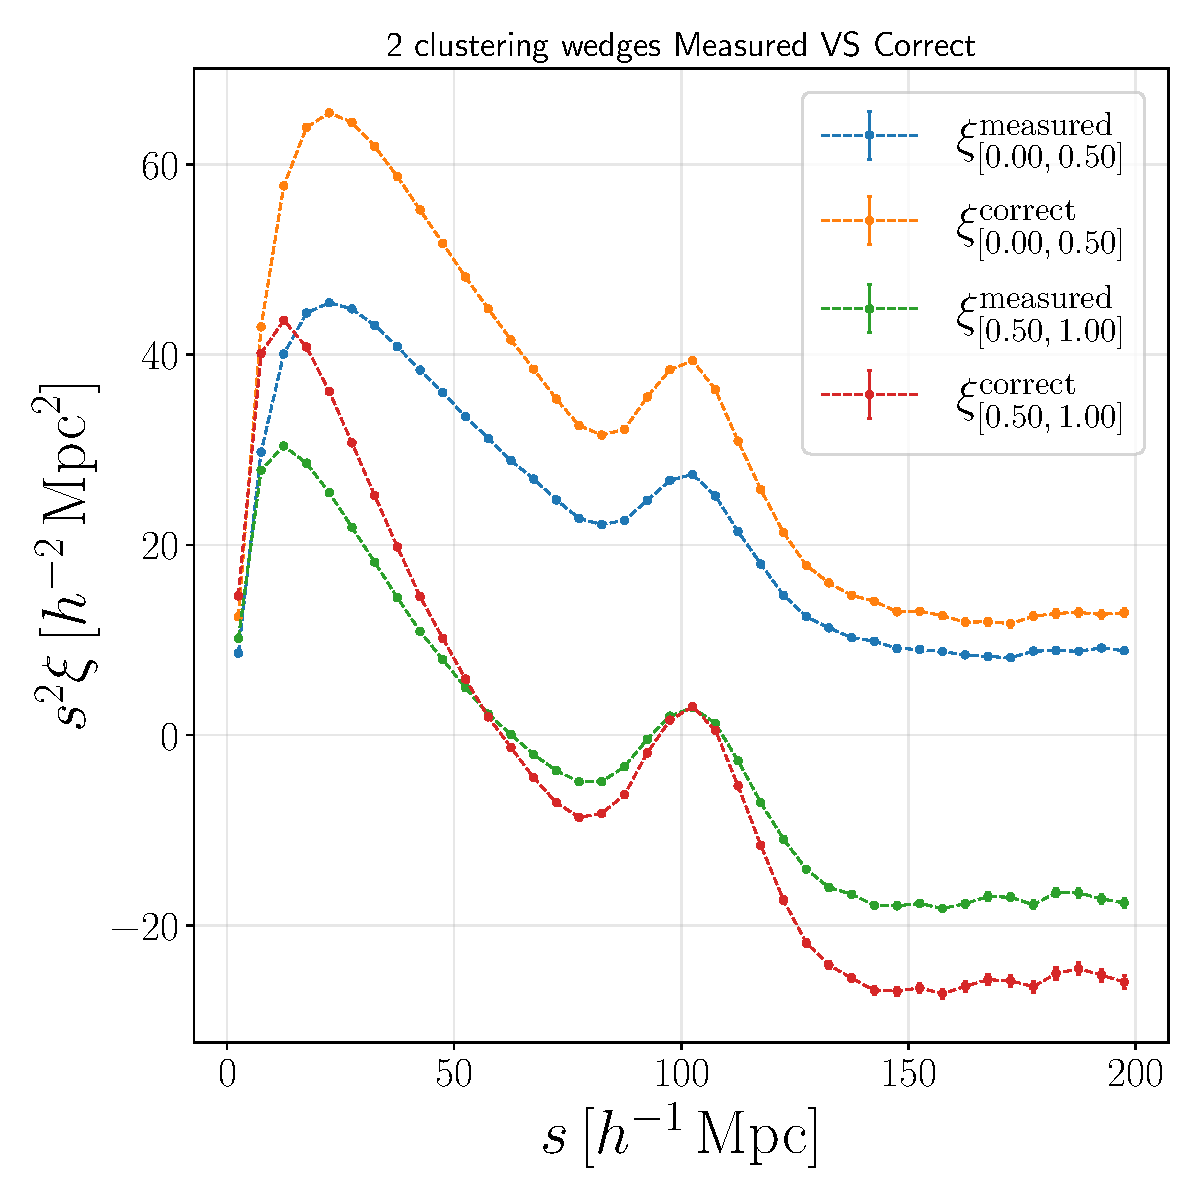
\includegraphics[width=\linewidth]{../graphs/z1_rebin/2clustWedges_measVScorr.pdf}
        \label{fig:ClusteringWedgesPlot_measVScorr_z1}
    \end{minipage}
    \hspace{0.5cm}
    \begin{minipage}{0.46\textwidth}
        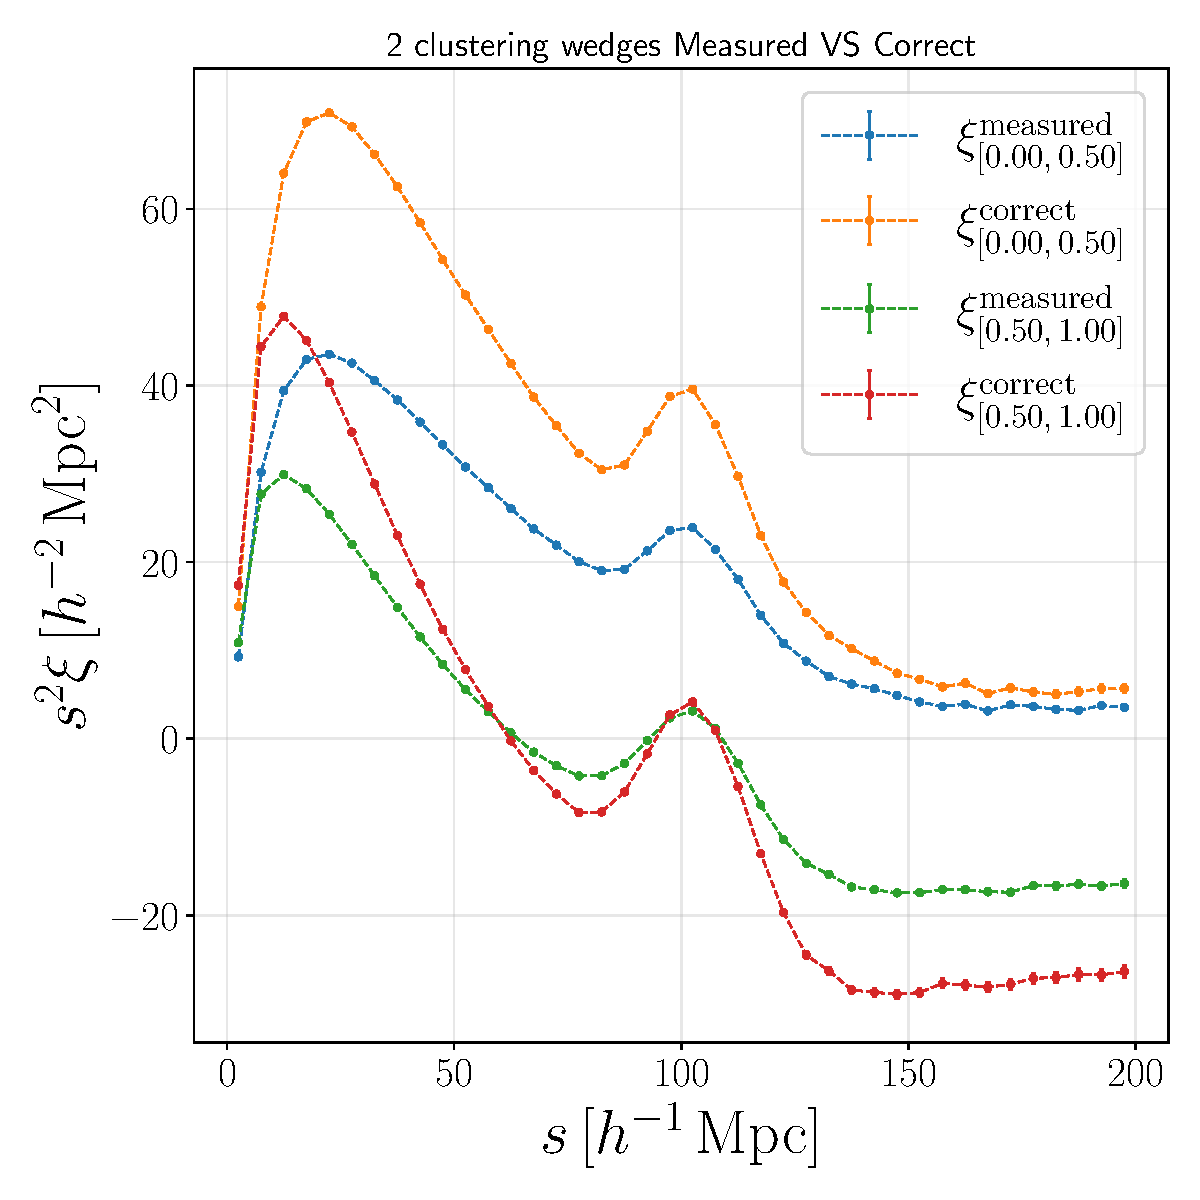
\includegraphics[width=\linewidth]{../graphs/z2_rebin/2clustWedges_measVScorr.pdf}
        \label{fig:ClusteringWedgesPlot_measVScorr_z2}
    \end{minipage}
    \caption{Plot showing the parallel and perpendicular wedges for the measured versus correct datasets for the redshift bin $z \in [0.9,1.1]$ in the left slot and $z \in [1.1,1.3]$ in the right slot.}
    \label{fig:ClusteringWedgesPlot_measVScorr_z1vsz2}
\end{figure}

\begin{figure}[!ht]
    \centering
    \begin{minipage}{0.46\textwidth}
        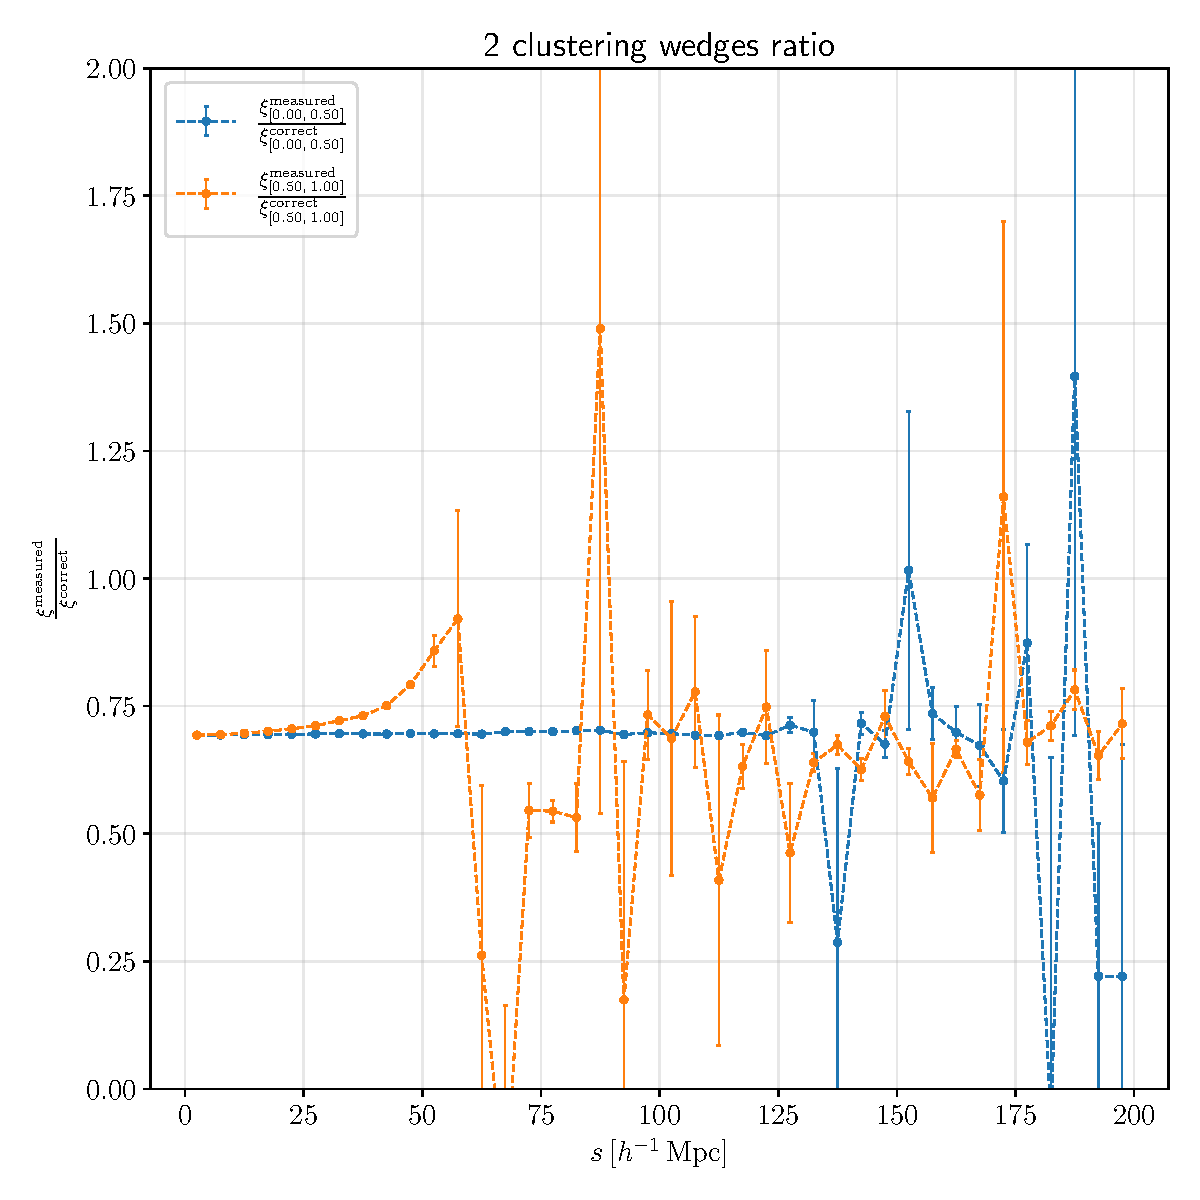
\includegraphics[width=\linewidth]{../graphs/z1_rebin/2clustWedge_ratio.pdf}
        \label{fig:ClusteringWedgesPlot_ratio_z1}
    \end{minipage}
    \hspace{0.5cm}
    \begin{minipage}{0.46\textwidth}
        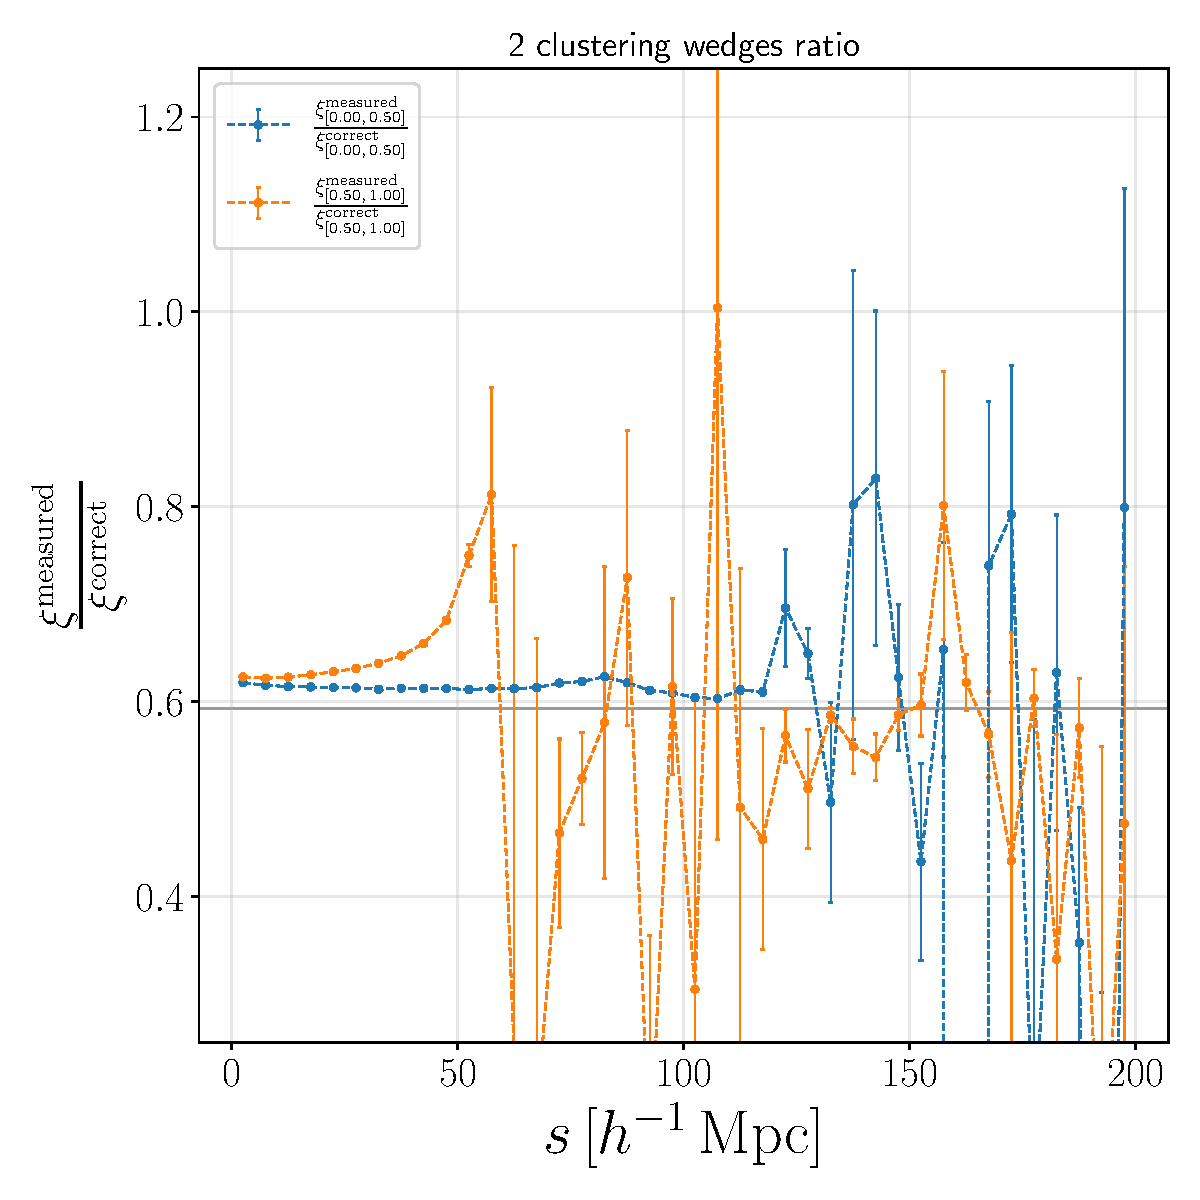
\includegraphics[width=\linewidth]{../graphs/z2_rebin/2clustWedge_ratio.pdf}
        \label{fig:ClusteringWedgesPlot_ratio_z2}
    \end{minipage}
    \caption{Plot showing the clustering wedges ratio between the measured and the correct datasets for the redshift bin $z \in [0.9,1.1]$ in the left slot and $z \in [1.1,1.3]$ in the right slot.}
    \label{fig:ClusteringWedgesPlot_ratio_z1vsz2}
\end{figure}

\begin{figure}[!ht]
    \centering
    \begin{minipage}{0.46\textwidth}
        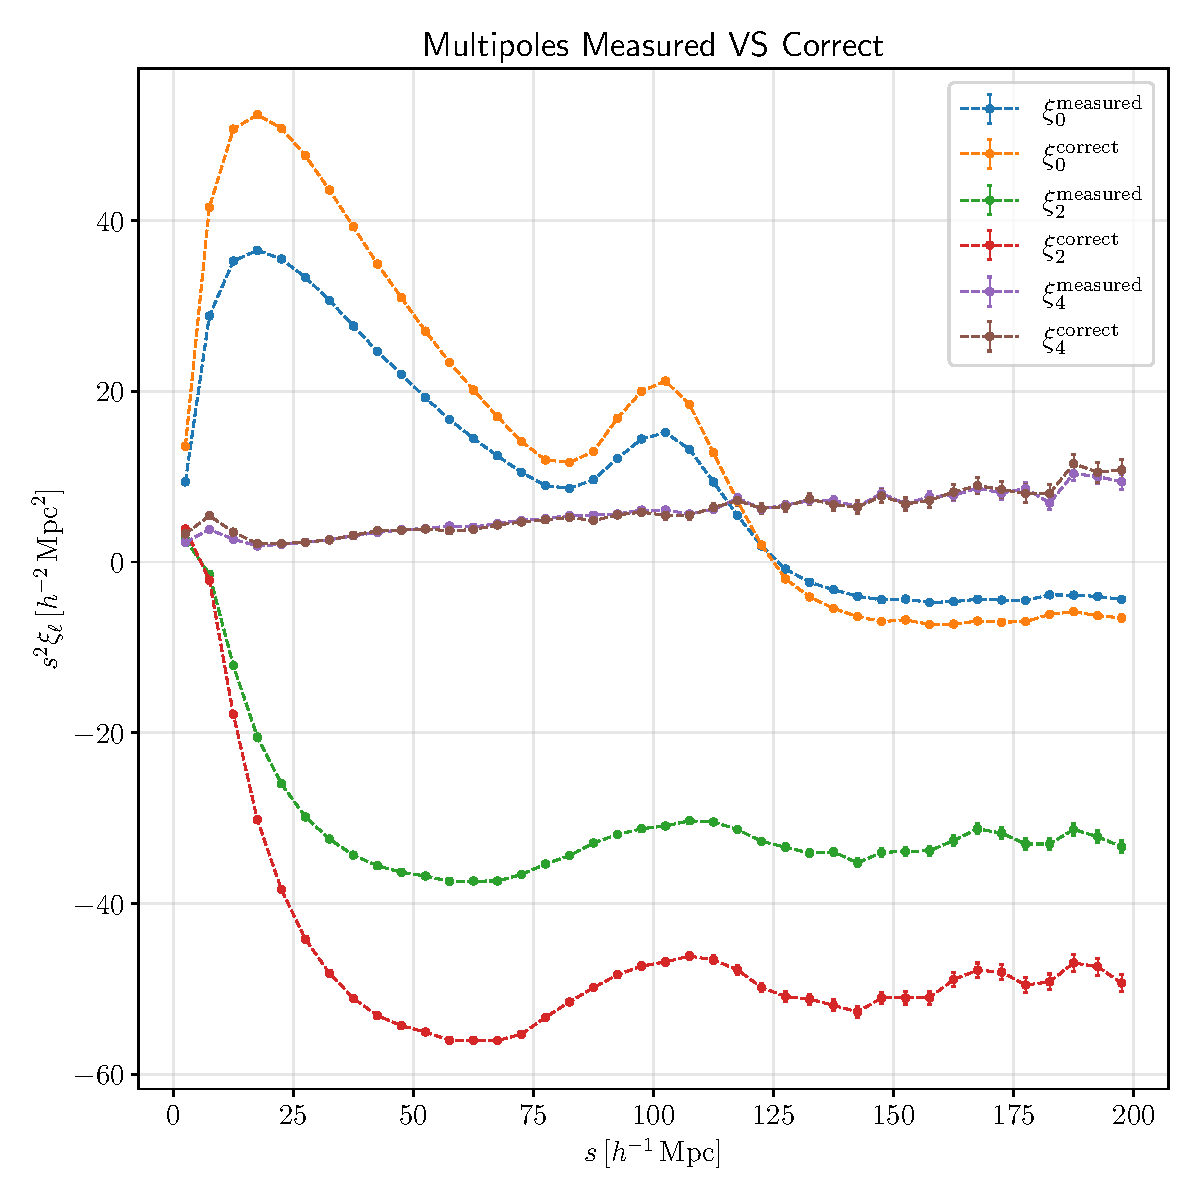
\includegraphics[width=\linewidth]{../graphs/z1_rebin/multipoles_measVScorr.pdf}
        \label{fig:MultipolesPlot_measVScorr_z1}
    \end{minipage}
    \hspace{0.5cm}
    \begin{minipage}{0.46\textwidth}
        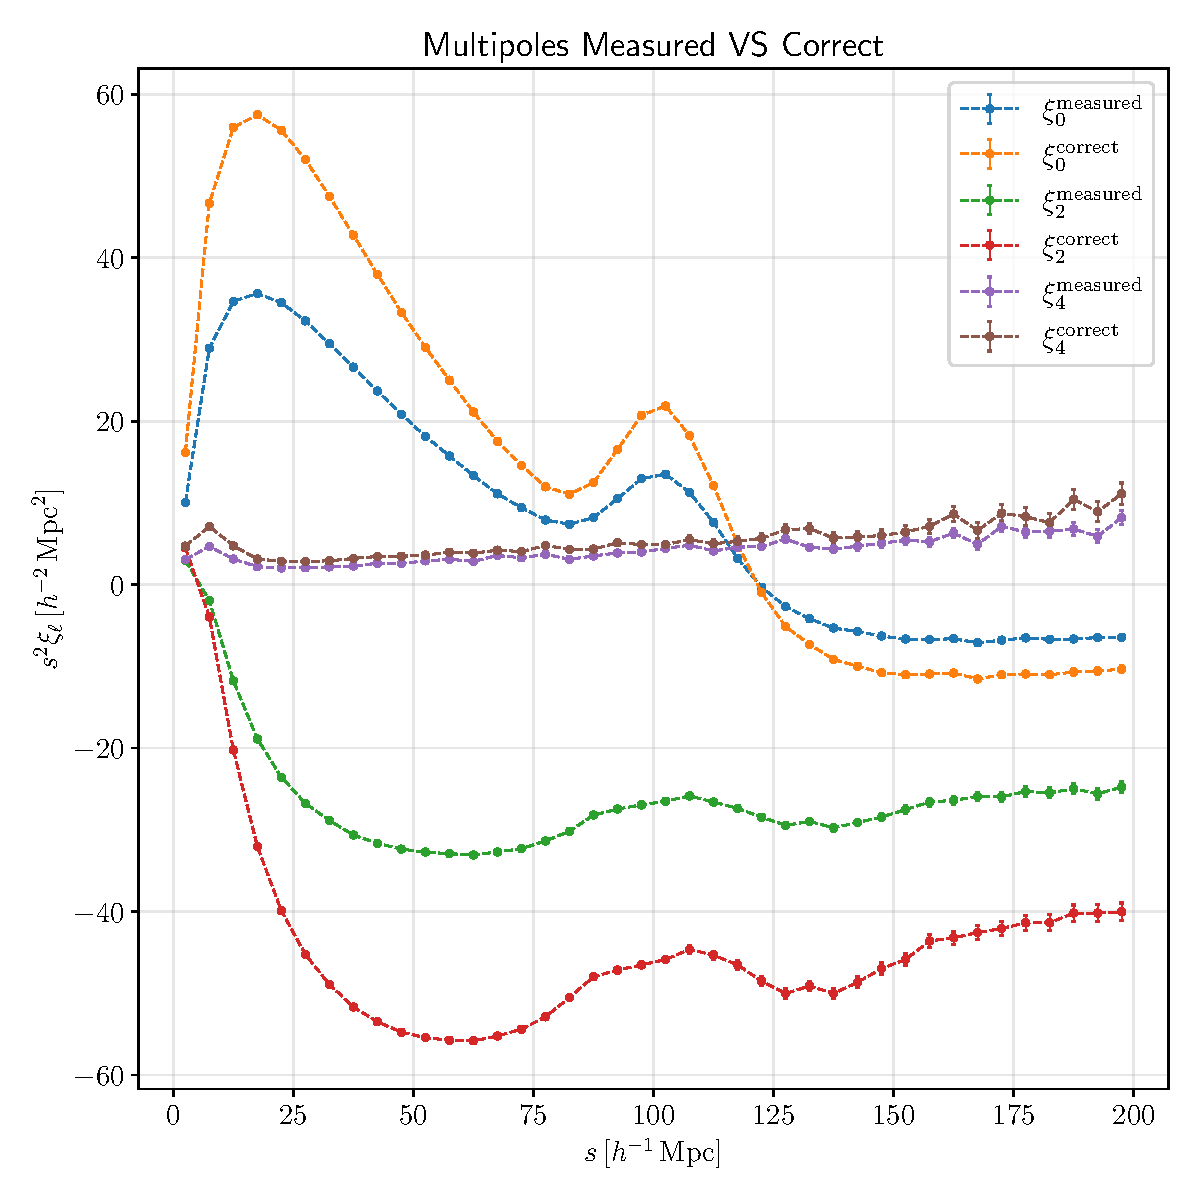
\includegraphics[width=\linewidth]{../graphs/z2_rebin/multipoles_measVScorr.pdf}
        \label{fig:MultipolesPlot_measVScorr_z2}
    \end{minipage}
    \caption{Plot showing the monopole, quadrupole and hexadecapole for the measured versus correct datasets for the redshift bin $z \in [0.9,1.1]$ in the left slot and $z \in [1.1,1.3]$ in the right slot.}
    \label{fig:MultipolesPlot_measVScorr_z1vsz2}
\end{figure}

\begin{figure}[!ht]
    \centering
    \begin{minipage}{0.46\textwidth}
        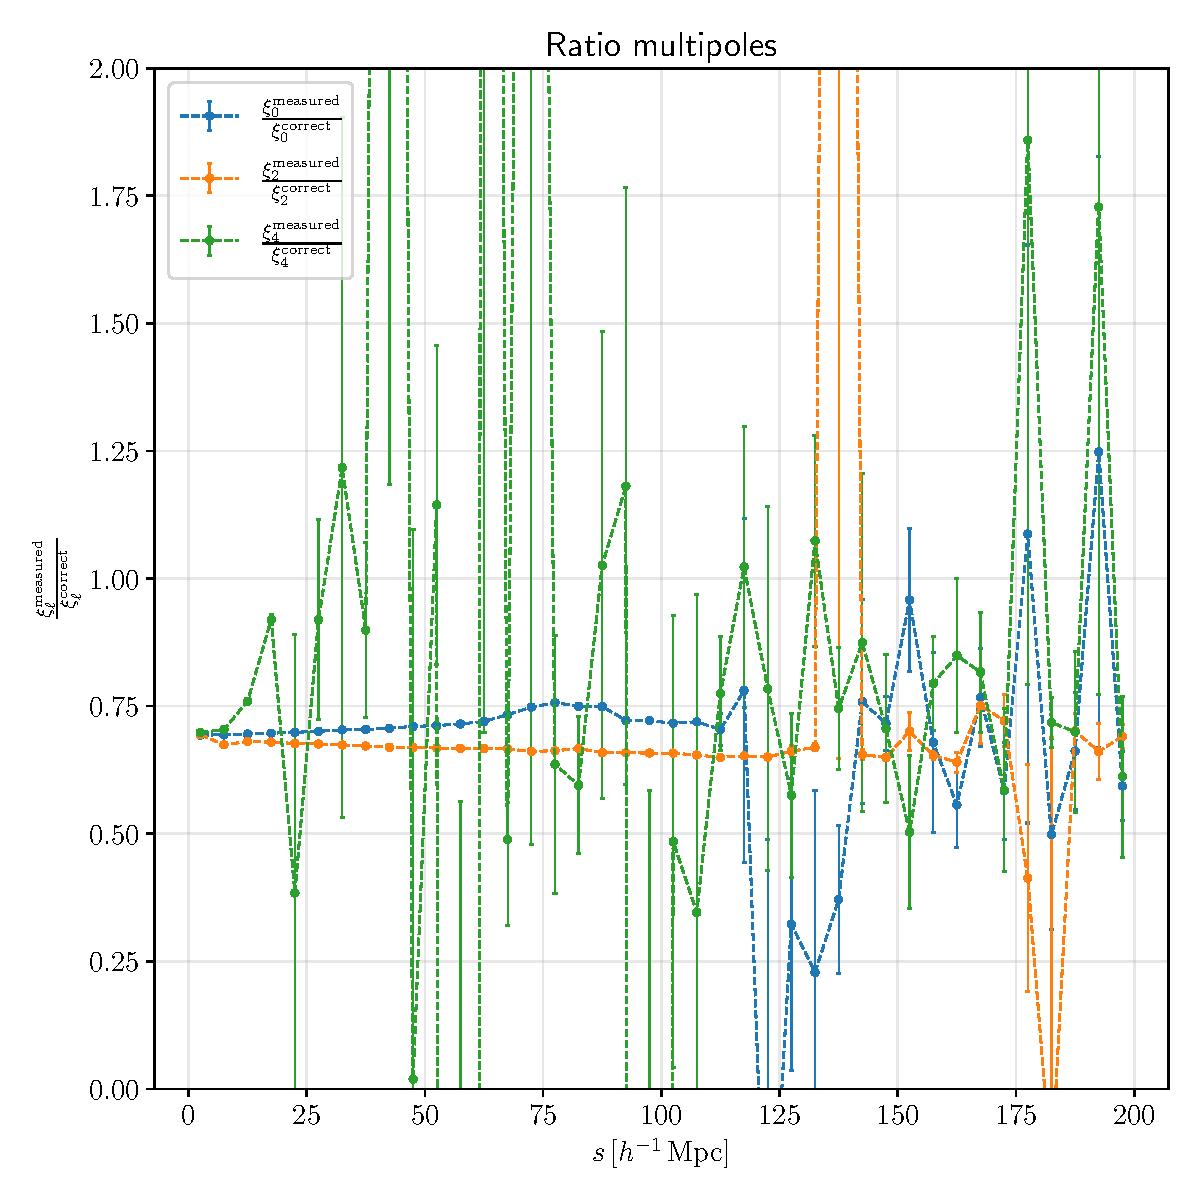
\includegraphics[width=\linewidth]{../graphs/z1_rebin/multipoles_ratio.pdf}
        \label{fig:MultipolesPlot_ratio_z1}
    \end{minipage}
    \hspace{0.5cm}
    \begin{minipage}{0.46\textwidth}
        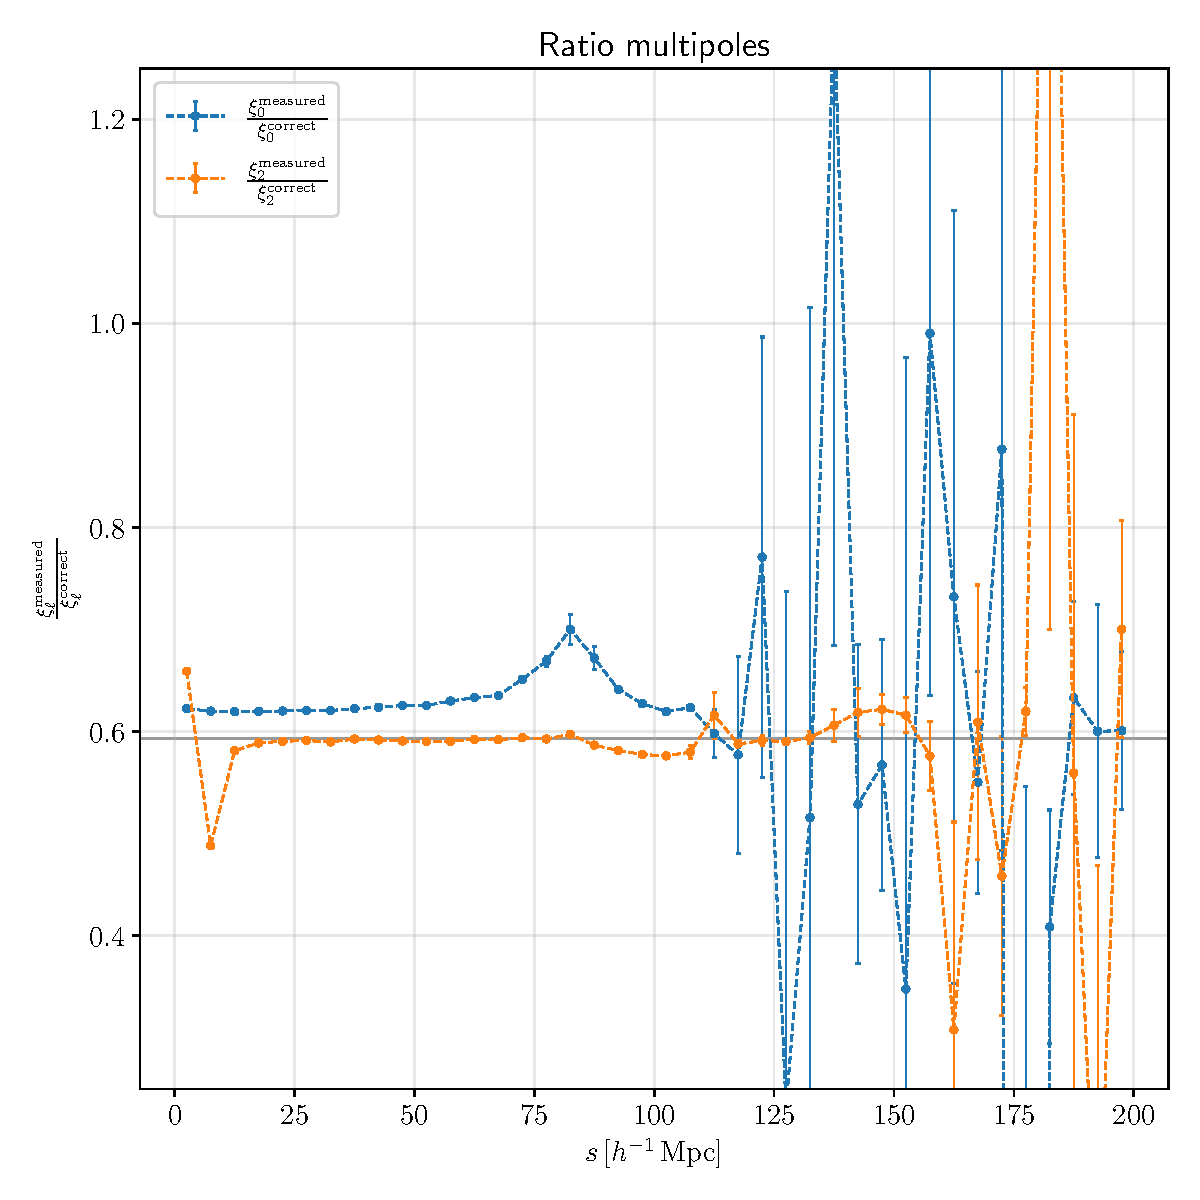
\includegraphics[width=\linewidth]{../graphs/z2_rebin/multipoles_ratio.pdf}
        \label{fig:MultipolesPlot_ratio_z2}
    \end{minipage}
    \caption{Plot showing the monopole and quadrupole ratio between the measured and the correct datasets for the redshift bin $z \in [0.9,1.1]$ in the left slot and $z \in [1.1,1.3]$ in the right slot.}
    \label{fig:MultipolesPlot_ratio_z1vsz2}
\end{figure}

A significant general pattern visible on small scales ($s < 40 \, h^{-1}\mathrm{Mpc}$) is that the ratio of the measured value to the correct one converges exactly to a specific value. This indicates a overall uniform suppression of the amplitude: it reflects the presence of interlopers in the sample. In fact, this attenuation assumes a dependence of the form
\begin{equation}
  \xi^\mathrm{measured} = (1-f_\mathrm{tot})^2 \, \xi^\mathrm{correct} \; ,
  \label{eq:InterloperSuppression}
\end{equation}
where $f_\mathrm{tot}$ is the total fraction of interlopers in each redshift bin and was defined earlier in Sec.~\ref{sec:Dataset}. While this is a simplified model, a more exhaustive analysis can be found in~\cite{IlariaR}.

\paragraph{Clustering wedges}
We can see that, for the transverse clustering wedge $\bar{\xi}_{\perp}(s)$, the ratio remains nearly constant and stable at around the factor $(1+f_\mathrm{tot})^2$, represented in the figure as a grey horizontal line, throughout almost the entire quasi-linear regime ($0 < s < 110 \, h^{-1}\mathrm{Mpc}$). This is what we could expect for the perpendicular wedge as the as contamination from interlopers in a slitless survey primarily causes a radial displacement of galaxies along the line-of-sight, thus leaving their angular positions in the sky intact. On the other hand the parallel wedge, rather than a simple drop in amplitude, shows a considerable difference in shape between the measured signal and the correct one. The ratio plot for this wedge confirms this by being highly scale-dependent, deviating from the attenuation value.

The Baryon Acoustic Oscillation peak is clearly visible around $s \approx 100 \ h^{-1} \mathrm{Mpc}$ in both wedges. However, in the parallel wedge, the measured signal's peak is suppressed and its surrounding shape is distorted compared to the correct signal.

We also note that the ratio plot is significantly scale-dependant: it diverges significantly from a certain value onwards, for the parallel wedge at $s \gtrsim 50 \ h^{-1} \mathrm{Mpc}$ and for both wedges at $s > 130 \ h^{-1} \mathrm{Mpc}$. These values align precisely with the scales where the true correlation function approaches or crosses zero: this unstable behavior is a numerical artifact driven by near-zero division.

\paragraph{Multipoles expansion}
The multipole expansion shares the same characteristics as those observed in clustering wedges.

\section{Impact on parameters}\label{sec:ImpactParamaters}
By following the procedures described in Sec.~\ref{sec:ParameterInference}, we have obtained the posterior distributions of the free parameters for both models, CLEFT and CLPT, for each redshift and for every scale cut considered.

The most obvious systematic error lies in the estimation of the clustering amplitude, $A_\mathrm{s}$. Across all tested models and minimum fitting scales $s_\mathrm{min}$, the contaminated data consistently yields a underestimated $A_\mathrm{s}$ compared to the correct value. This behavior is a direct consequence of the scale-independent signal attenuation observed in the transverse clustering wedge: as interlopers suppress the overall amplitude of the correlation function by a factor $(1 - f_\mathrm{tot})^2$, the sampler incorrectly interprets this purely observational artifact as a universe with intrinsically weaker matter clustering.

Furthermore, the physical density of cold dark matter, $\omega_\mathrm{c}$, presents shifts in its posterior contours. Interlopers do not simply reduce the amplitude of the signal; anisotropic scattering also distorts the shape of the correlation function, in particular suppressing and broadening the peak of BAO along the line-of-sight. This distortion of the shape disrupts theoretical models, forcing shifts in $\omega_c$ as the model attempts to fit the modified broadband shape of the power spectrum.

The Hubble parameter, $h$, is, instead, more robust since we do not observe any strong discrepancy with the fiducial value in any of our cases.

Overall, 1D posterior distributions, displayed along the diagonal panels of the plots, show us the statistical behaviour of the model fits. For the primary cosmological parameters ($h$, $A_\mathrm{s}$, $\omega_\mathrm{c}$) and for the linear bias of galaxies ($1+b_1$), the one-dimensional contours are predominantly Gaussian. This generally symmetric, bell-shaped pattern indicates that the chains have converged well and that the sampler has identified a statistically stable region of parameter space; this means that the models are finding a highly reliable and stable fit to the data. Whilst the primary parameters remain largely Gaussian, a critical deviation occurs in the perturbation parameters that govern non-linearities and small-scale physics. In several cases, the 1D posterior distributions derived from measured data become highly non-Gaussian, strongly asymmetric, or even reach the limits of their uniformly distributed prior intervals. 

\begin{figure}[t]
    \centering
    \begin{minipage}{0.47\textwidth}
        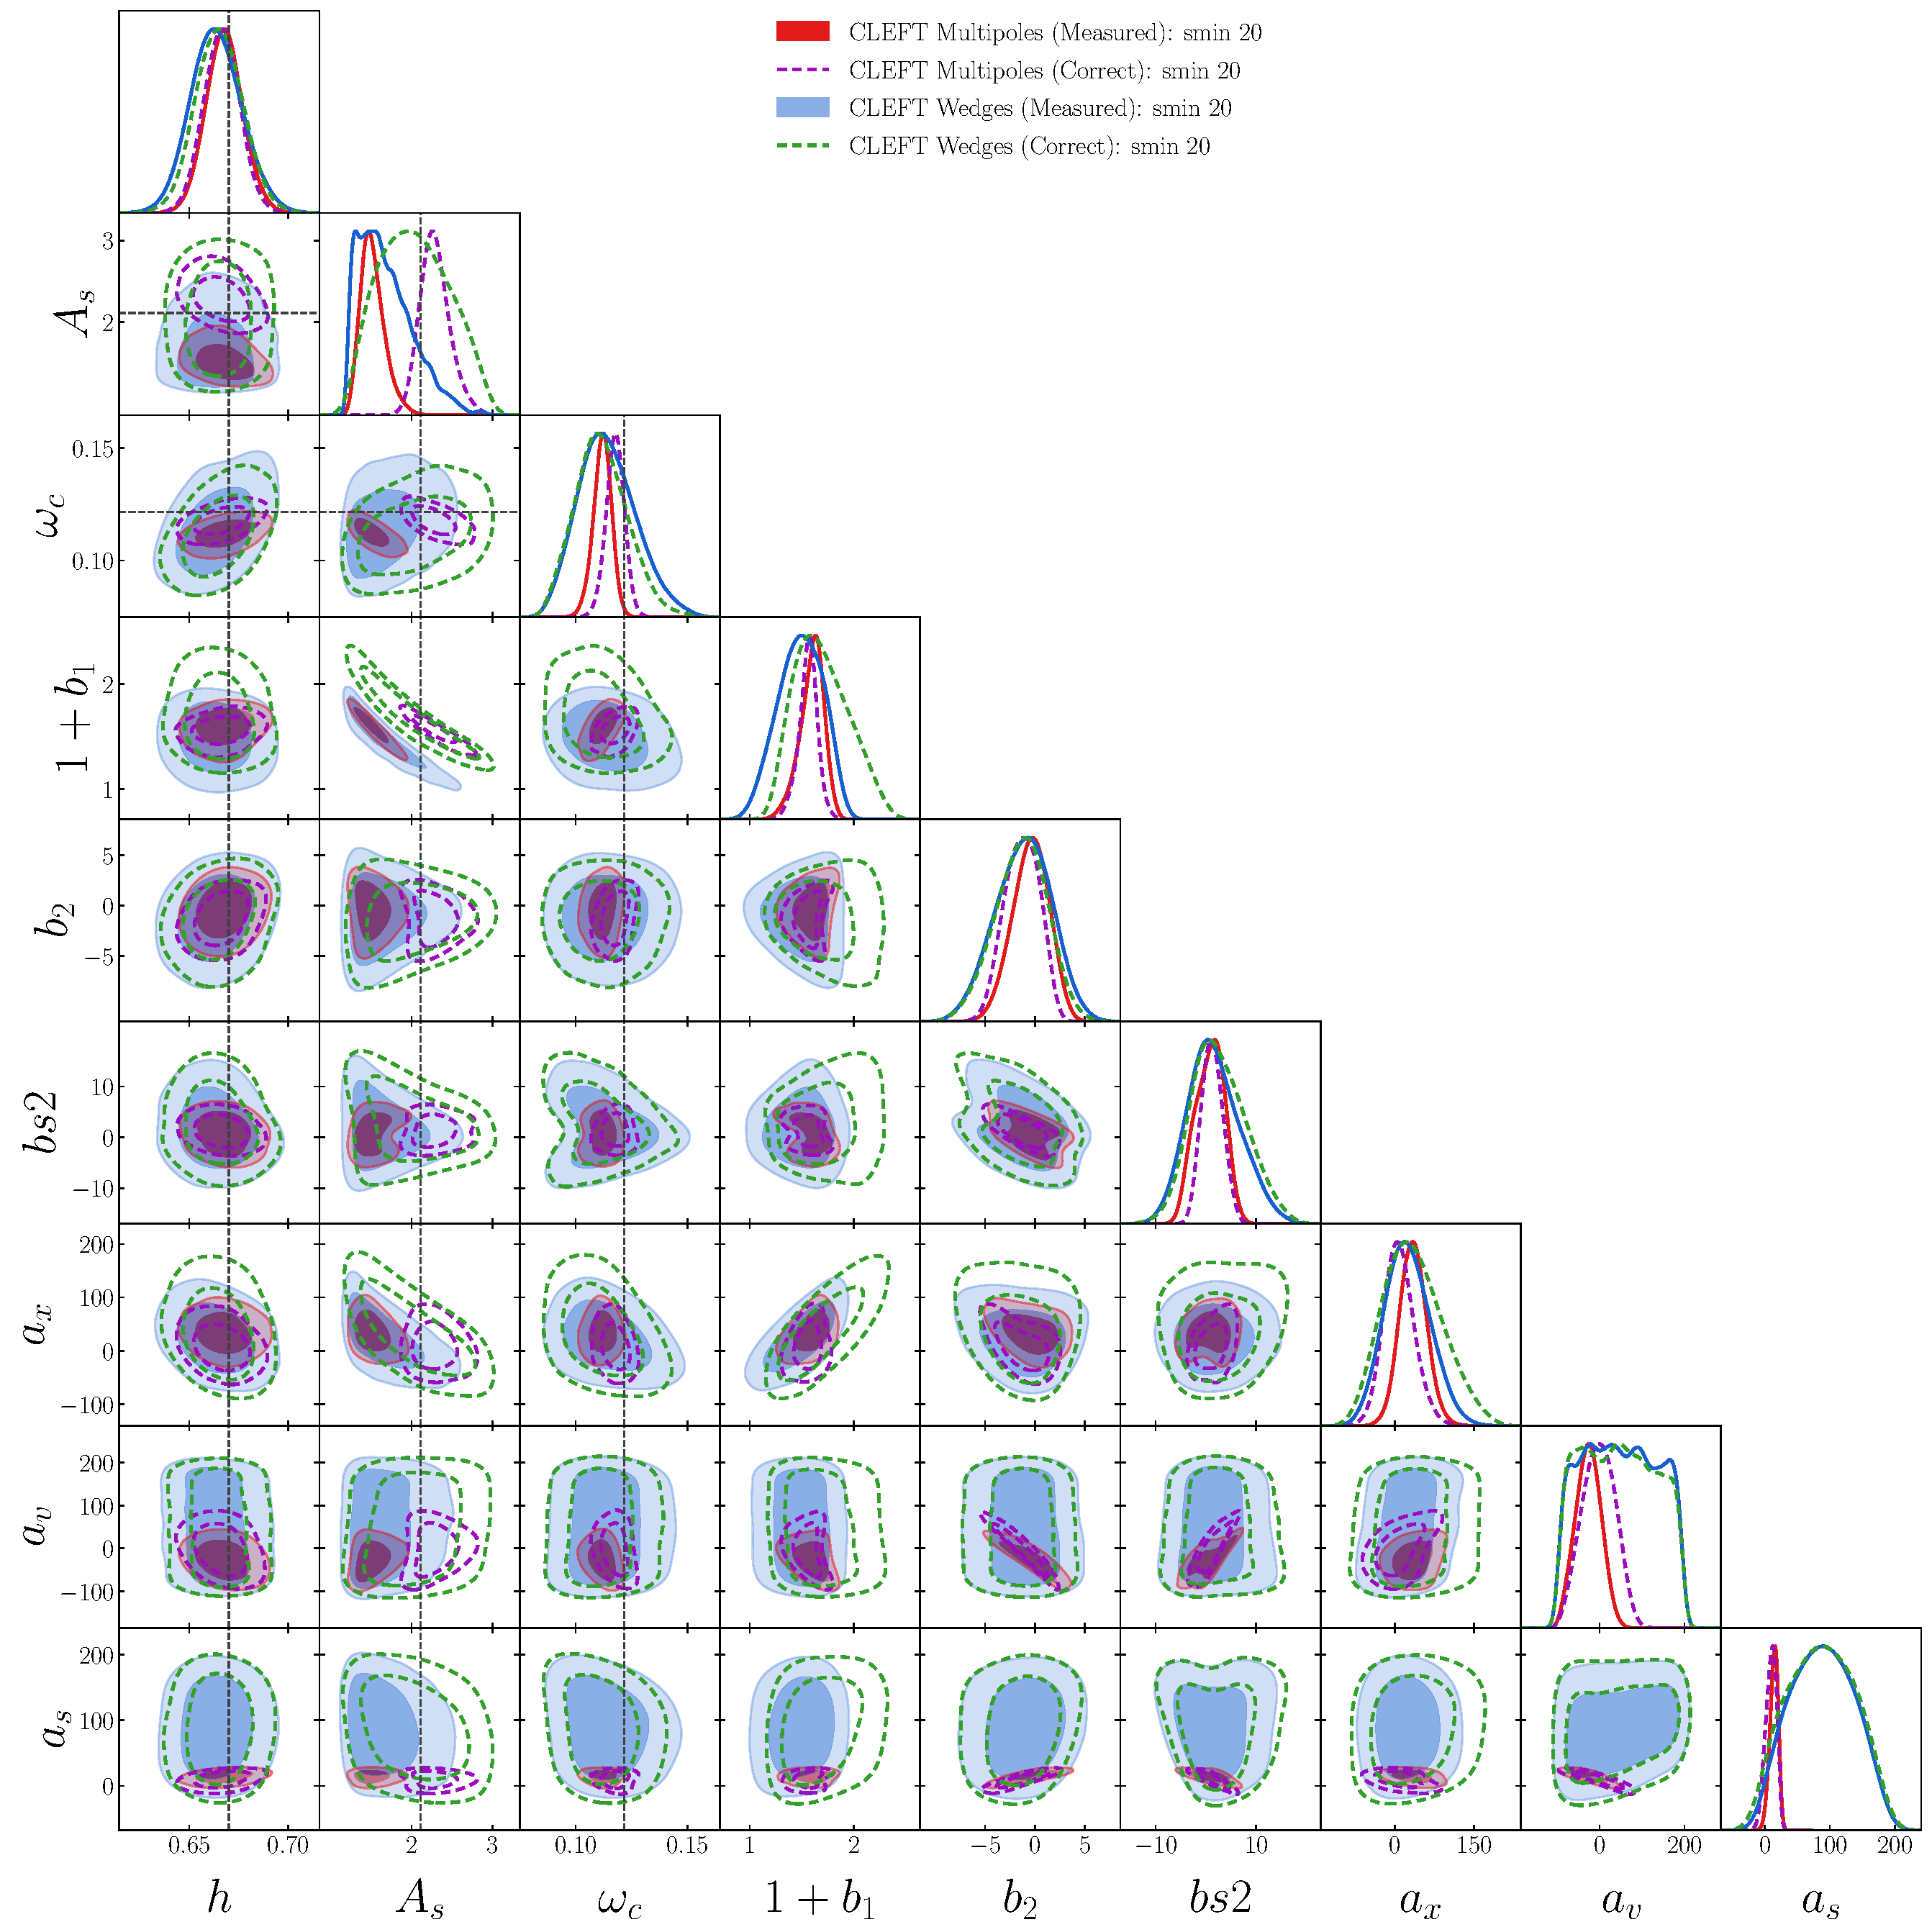
\includegraphics[width=\linewidth]{../graphs/z1_rebin/ELM_contours_CLEFT_smin_20_MMWW_MCMC.pdf}
        \label{fig:CLEFT_smin20_z1}
    \end{minipage}
    \hspace{0.5cm}
    \begin{minipage}{0.47\textwidth}
        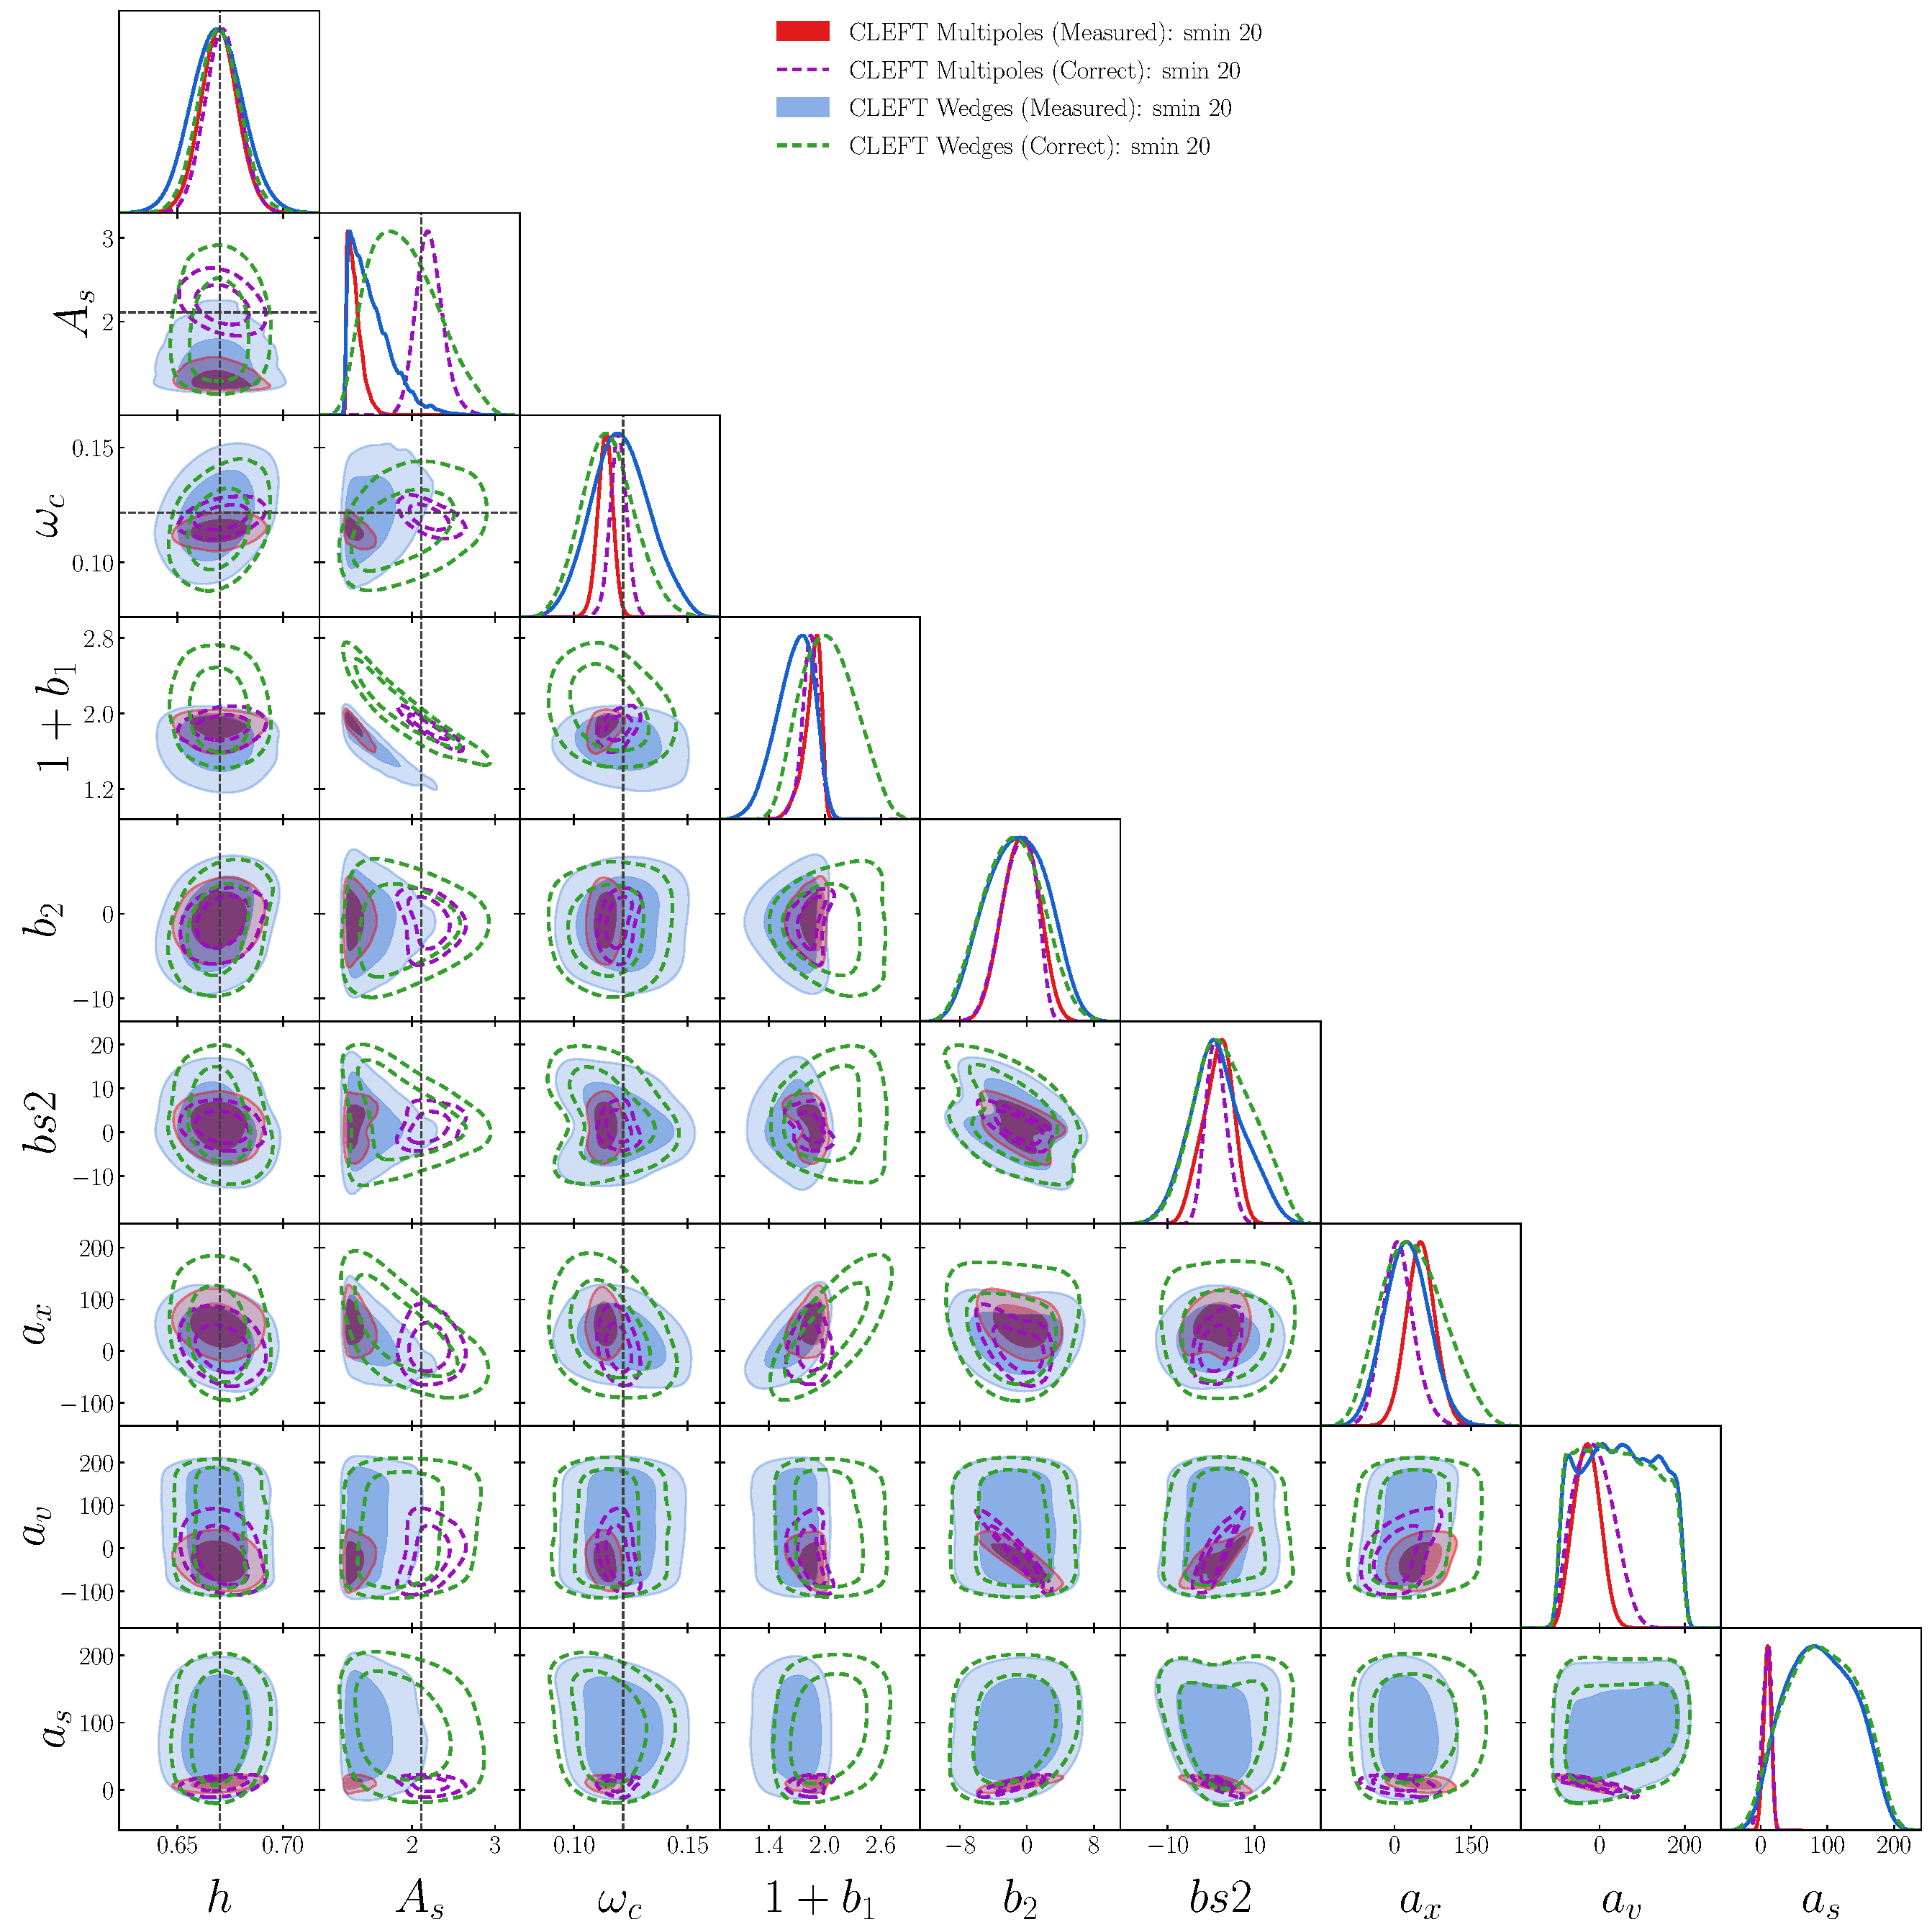
\includegraphics[width=\linewidth]{../graphs/z2_rebin/ELM_contours_CLEFT_smin_20_MMWW_MCMC.pdf}
        \label{fig:CLEFT_smin20_z2}
    \end{minipage}
    \caption{Contour plots for CLEFT model with scale-cut $s_\mathrm{min}=20 \, h^{-1}\mathrm{Mpc}$ for the redshift bin $z \in [0.9,1.1]$ in the left slot and $z \in [1.1,1.3]$ in the right slot.}
    \label{fig:CLEFT_smin20_z1vsz2}
\end{figure}
\begin{figure}[!ht]
    \centering
    \begin{minipage}{0.47\textwidth}
        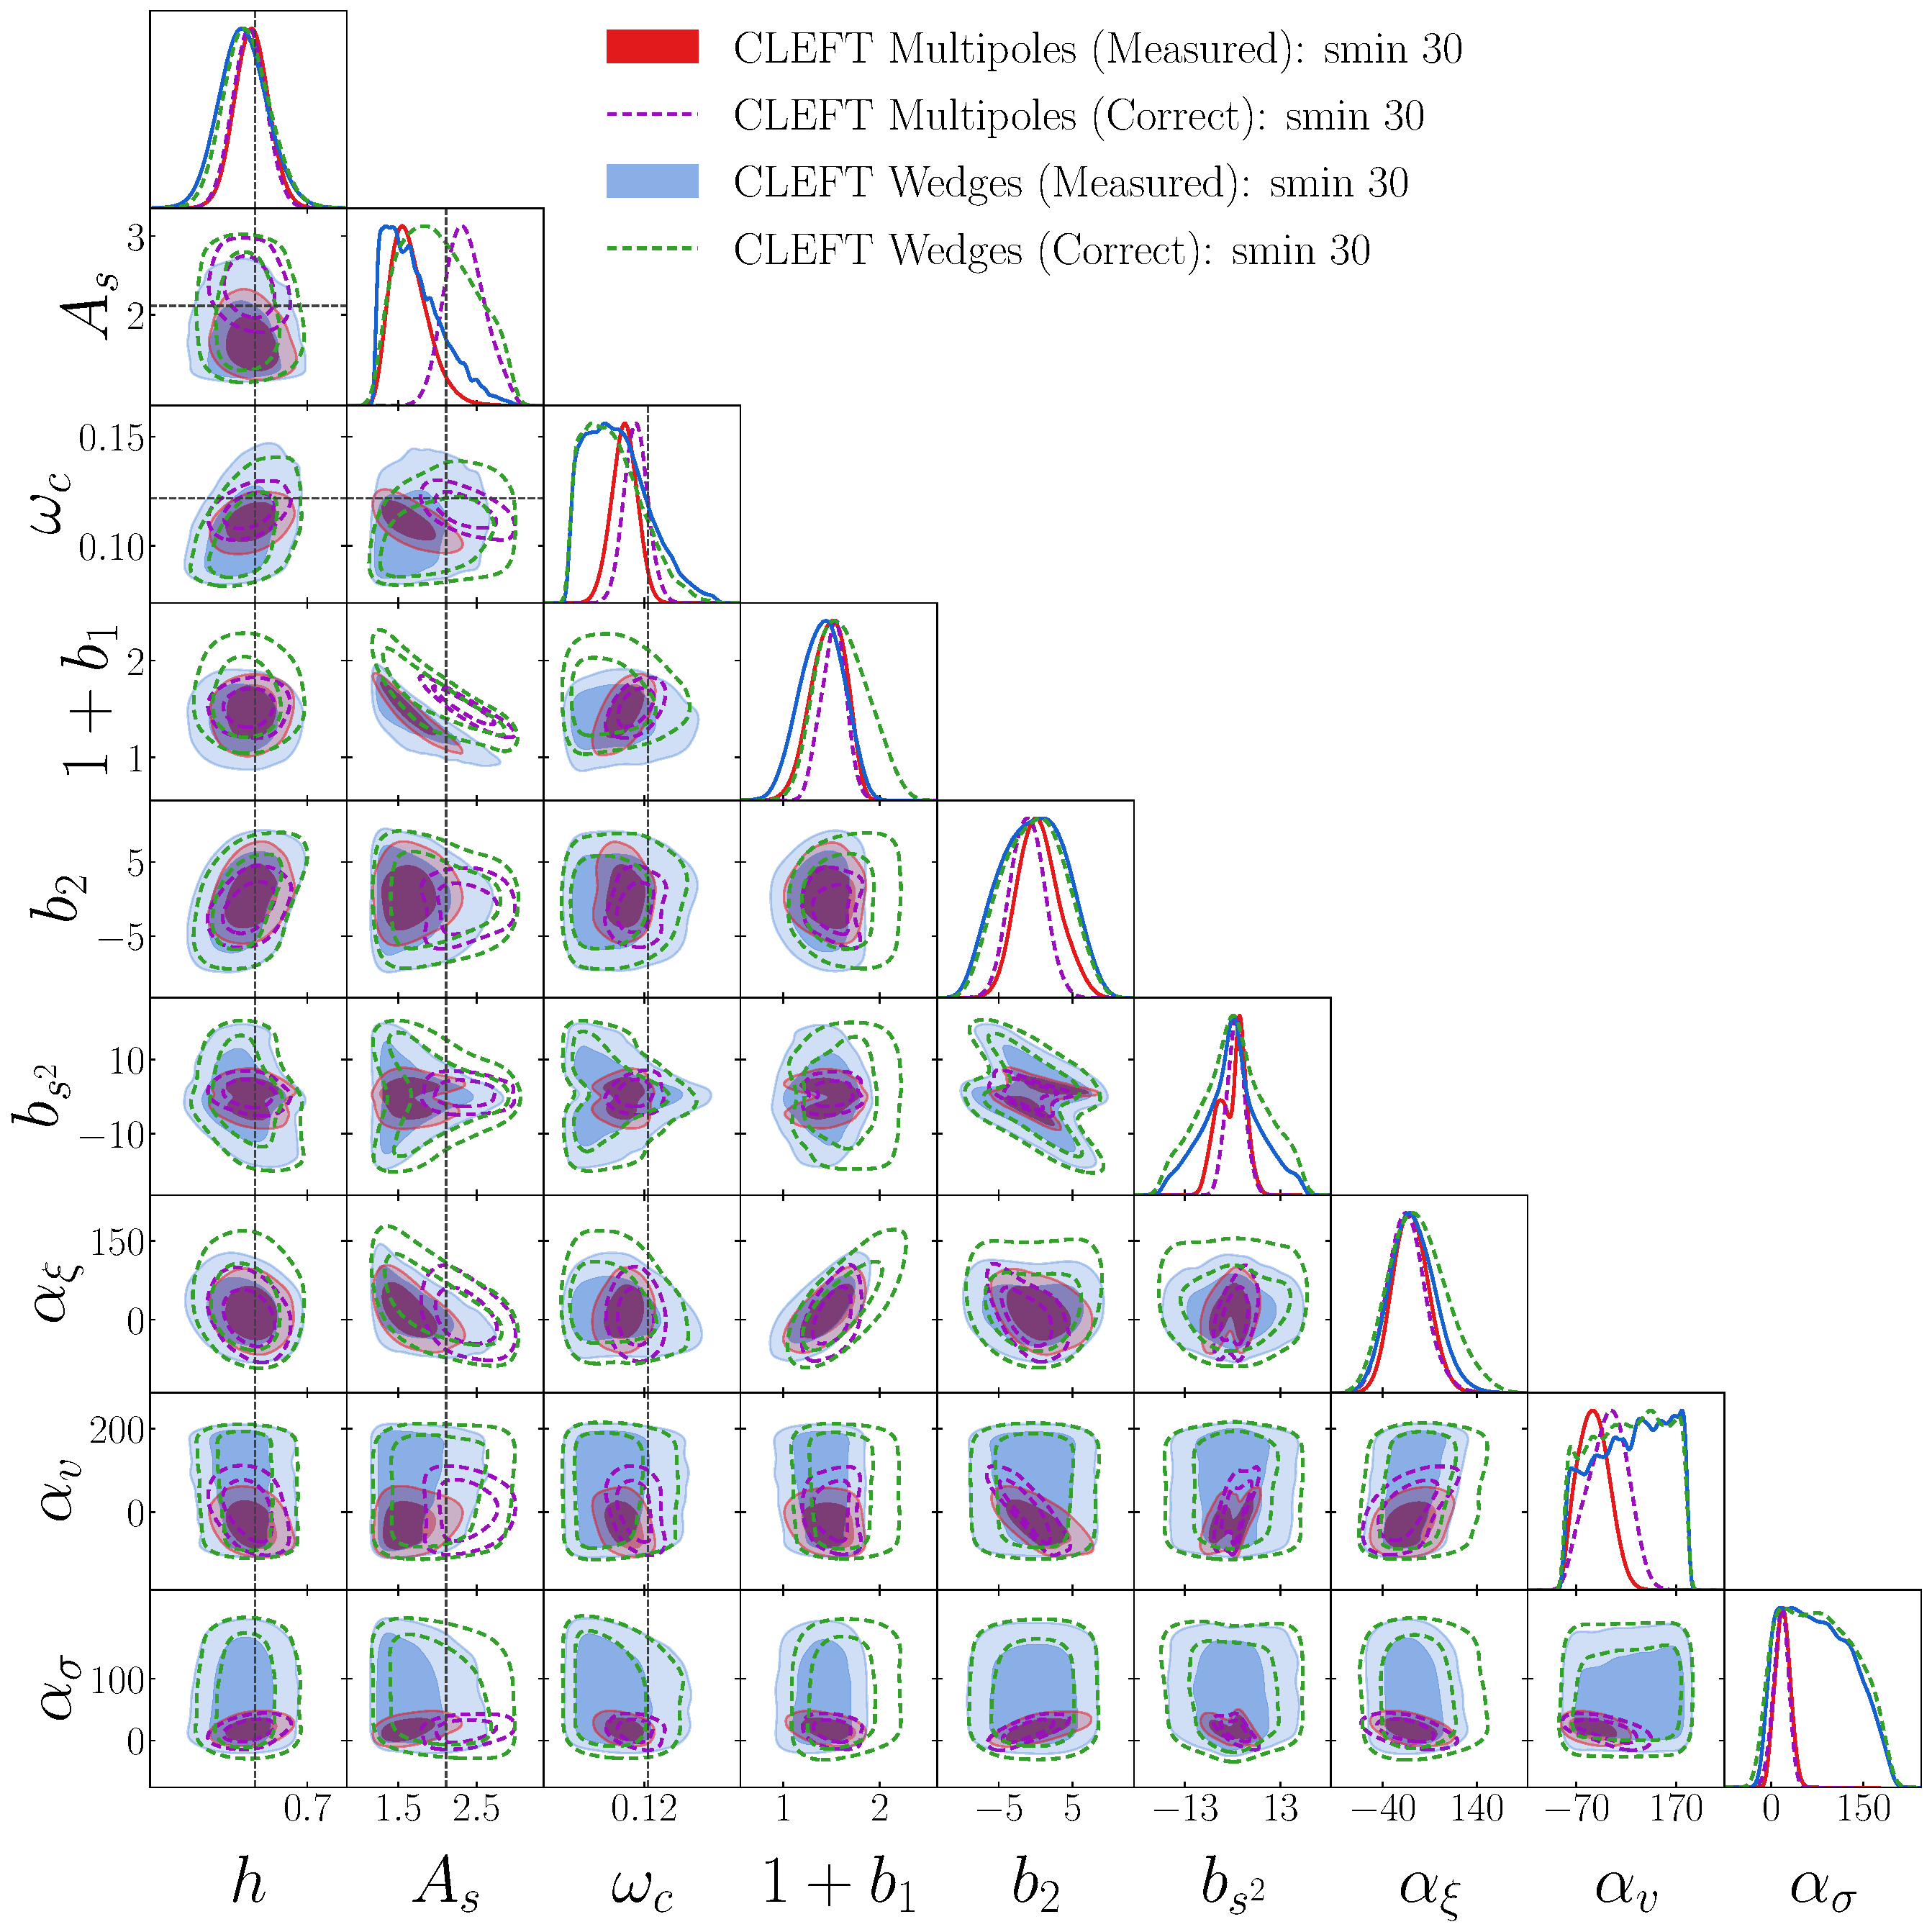
\includegraphics[width=\linewidth]{../graphs/z1_rebin/ELM_contours_CLEFT_smin_30_MMWW_MCMC.pdf}
        \label{fig:CLEFT_smin30_z1}
    \end{minipage}
    \hspace{0.5cm}
    \begin{minipage}{0.47\textwidth}
        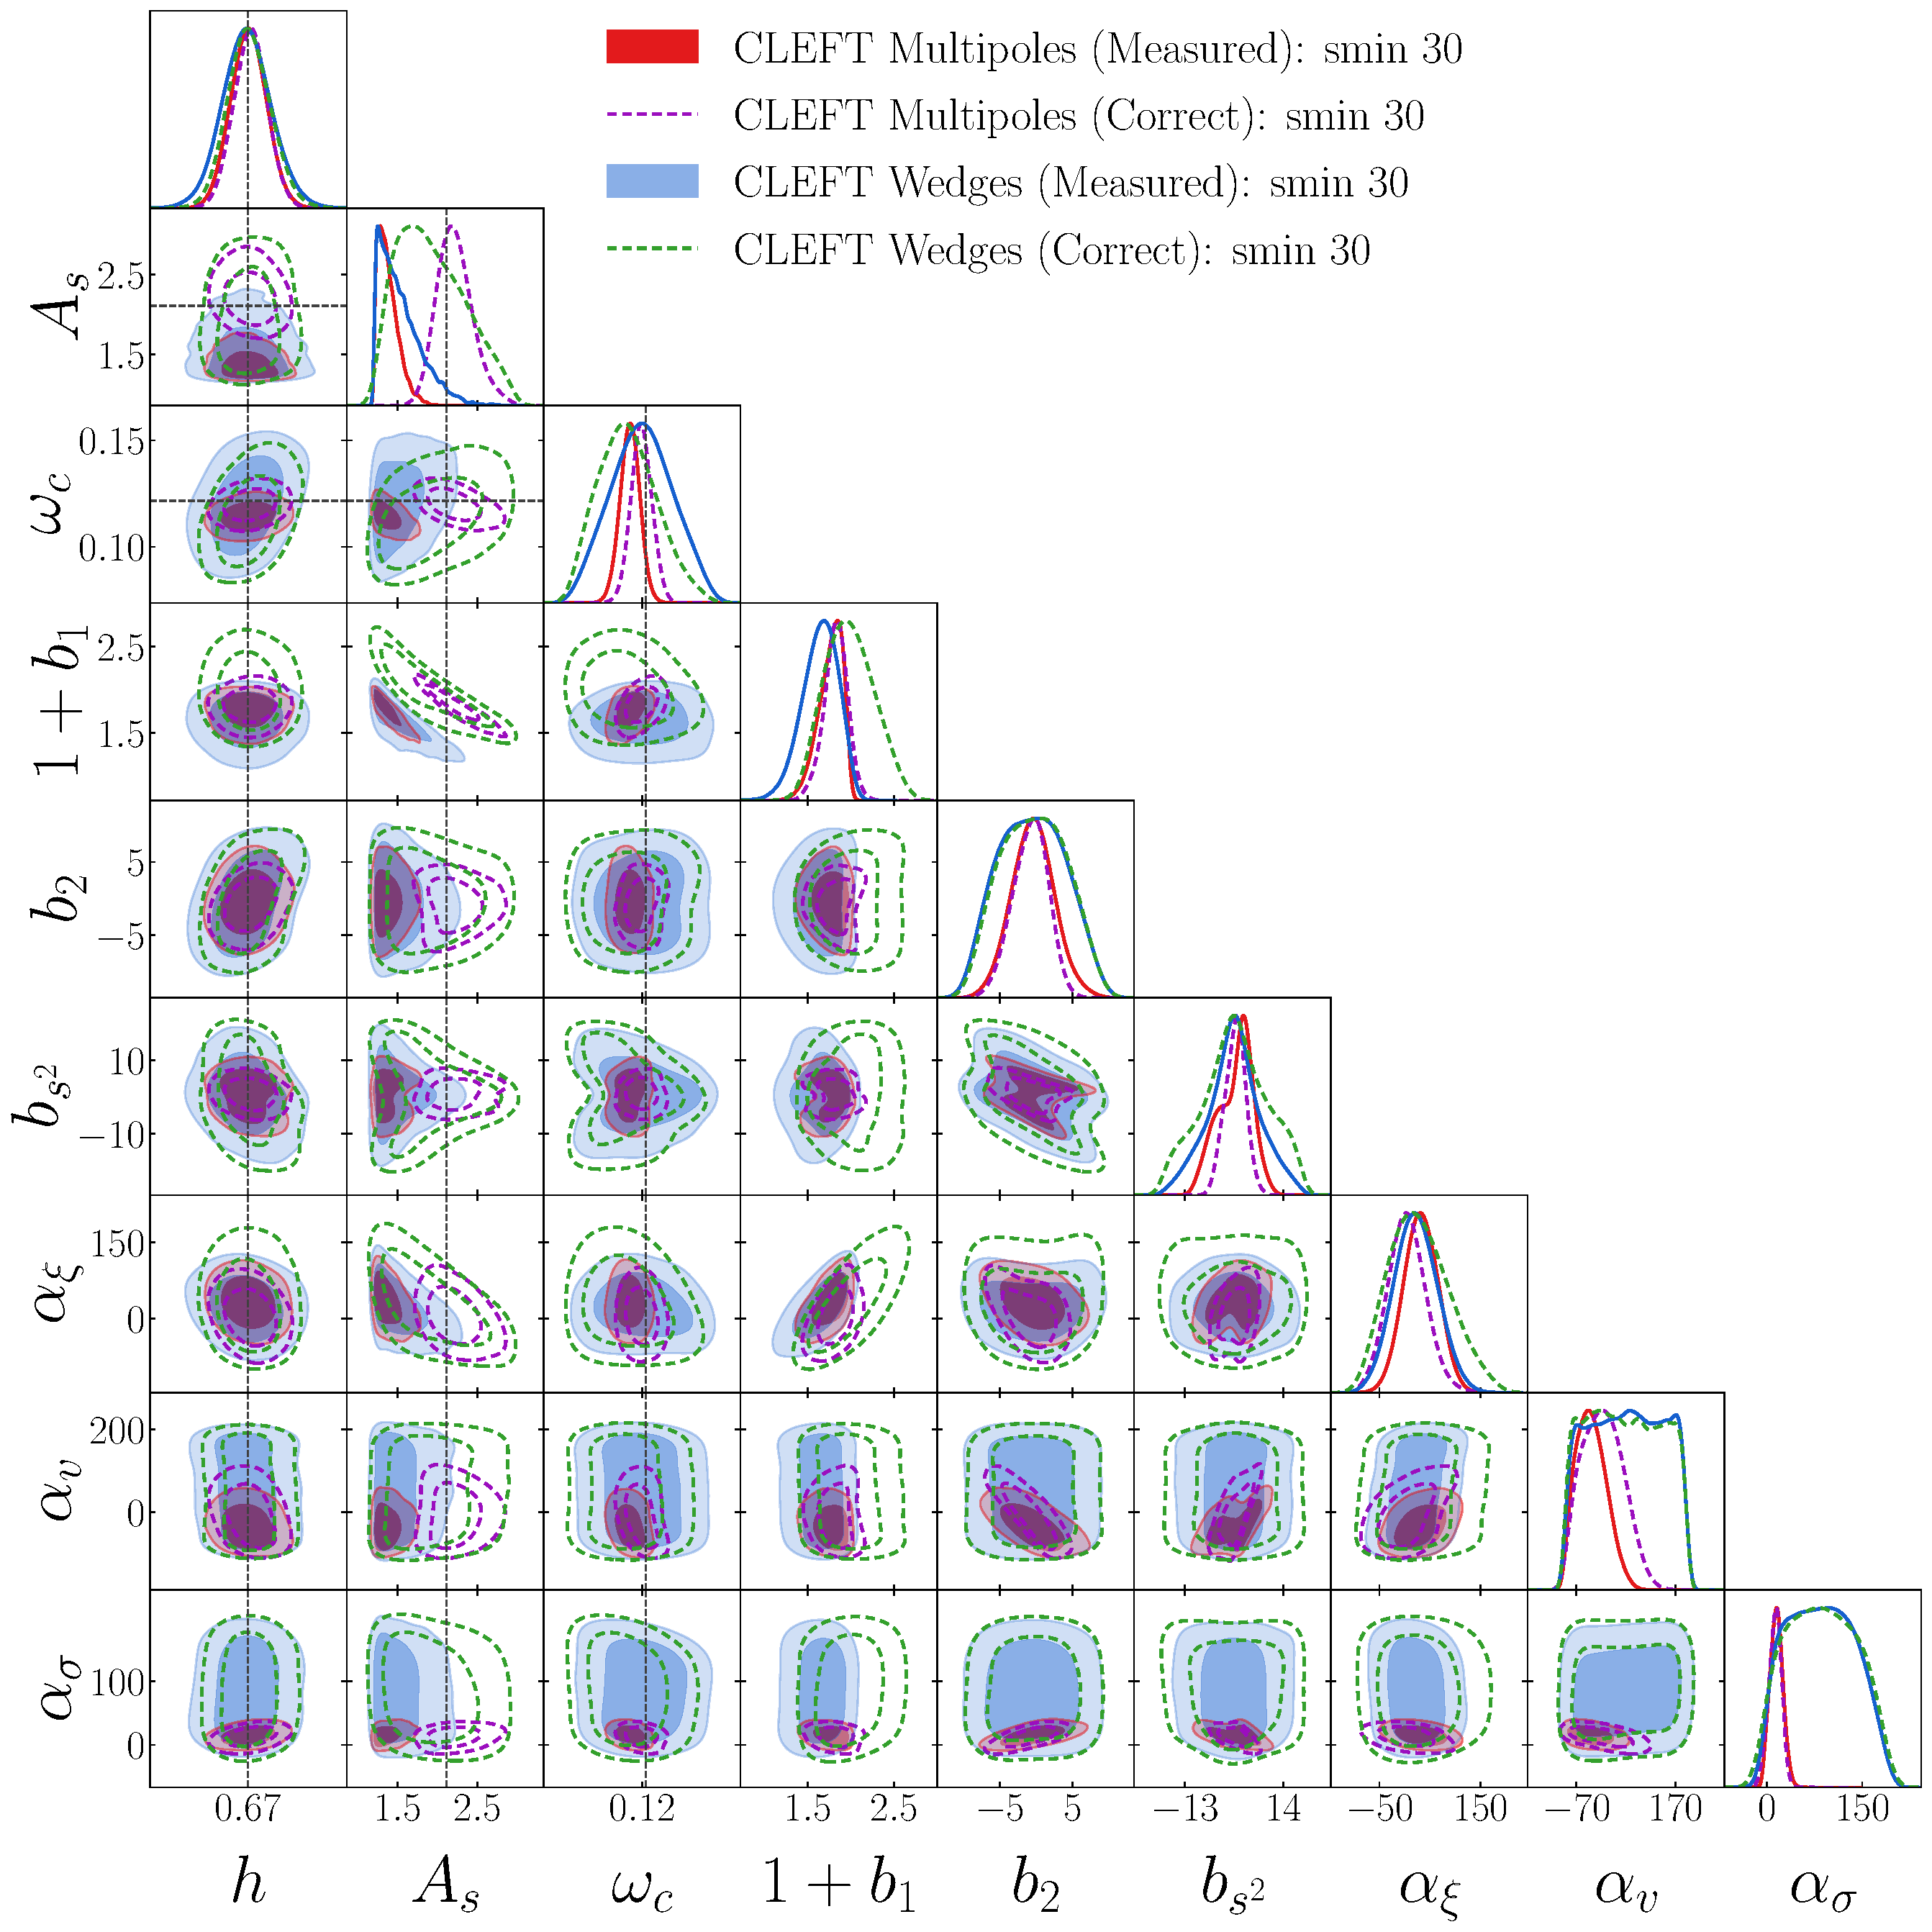
\includegraphics[width=\linewidth]{../graphs/z2_rebin/ELM_contours_CLEFT_smin_30_MMWW_MCMC.pdf}
        \label{fig:CLEFT_smin30_z2}
    \end{minipage}
    \caption{Contour plots for CLEFT model with scale-cut $s_\mathrm{min}=30 \, h^{-1}\mathrm{Mpc}$ for the redshift bin $z \in [0.9,1.1]$ in the left slot and $z \in [1.1,1.3]$ in the right slot.}
    \label{fig:CLEFT_smin30_z1vsz2}
\end{figure}
\begin{figure}[!ht]
    \centering
    \begin{minipage}{0.47\textwidth}
        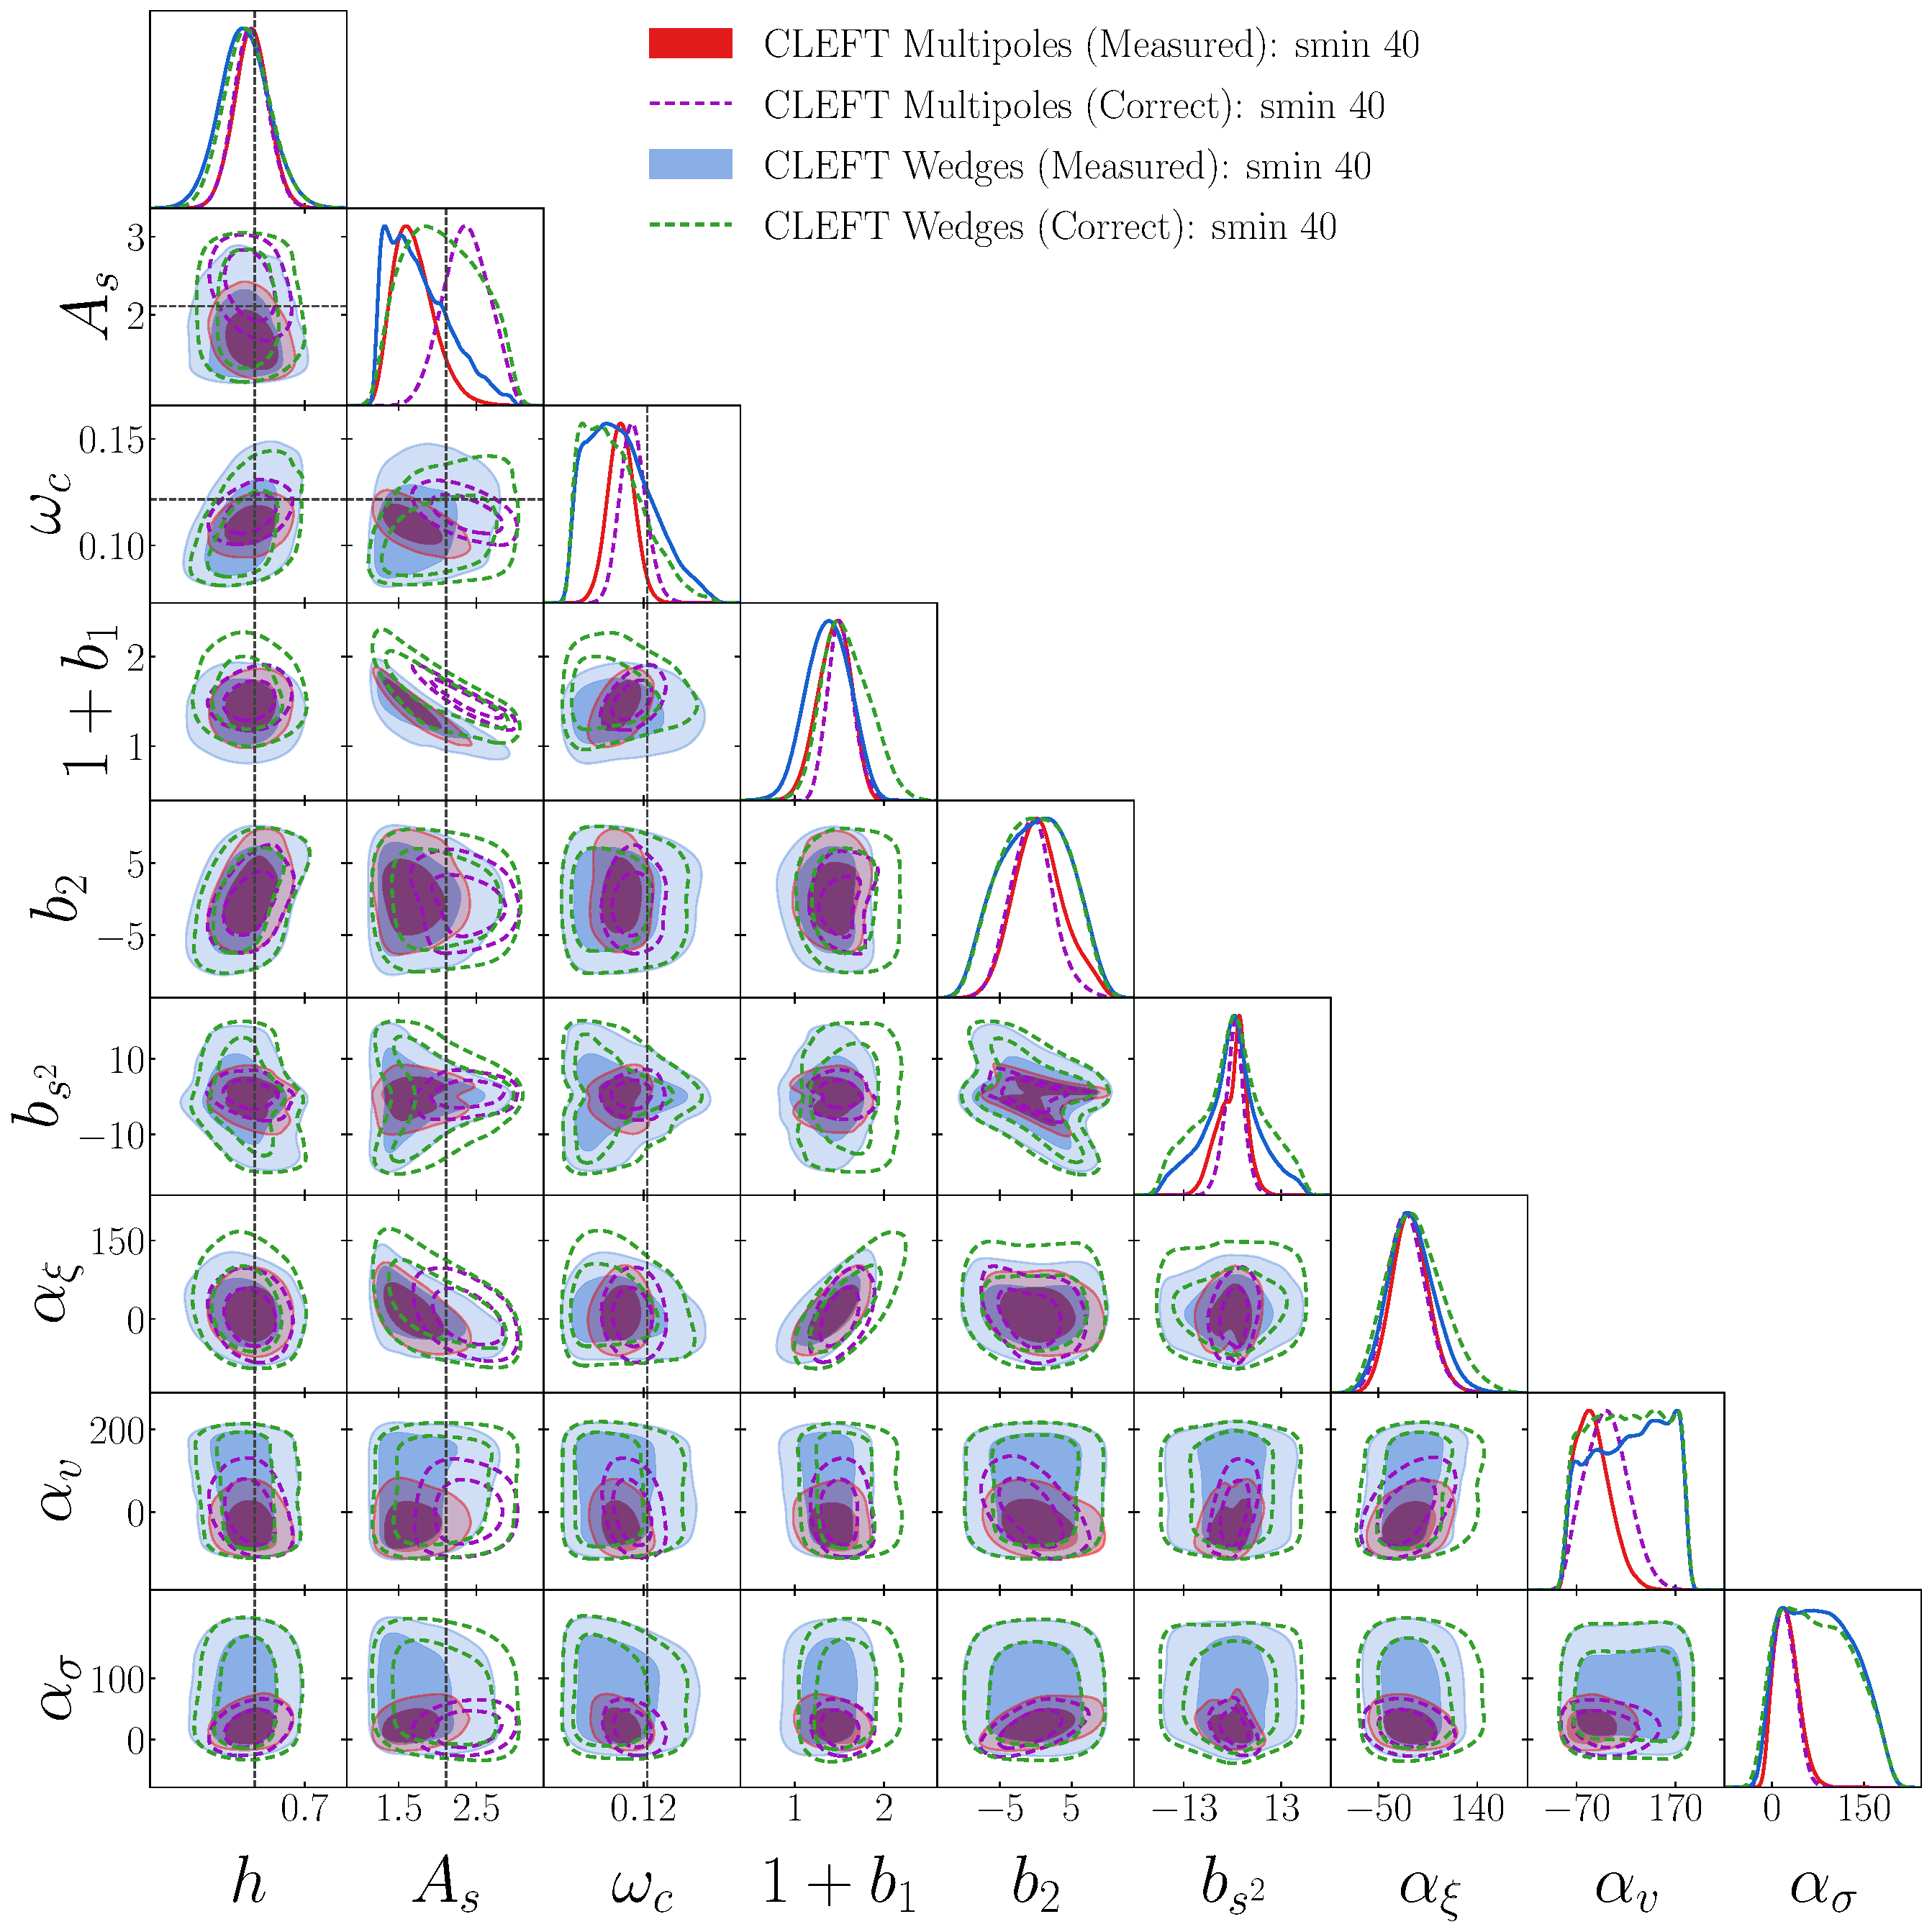
\includegraphics[width=\linewidth]{../graphs/z1_rebin/ELM_contours_CLEFT_smin_40_MMWW_MCMC.pdf}
        \label{fig:CLEFT_smin40_z1}
    \end{minipage}
    \hspace{0.5cm}
    \begin{minipage}{0.47\textwidth}
        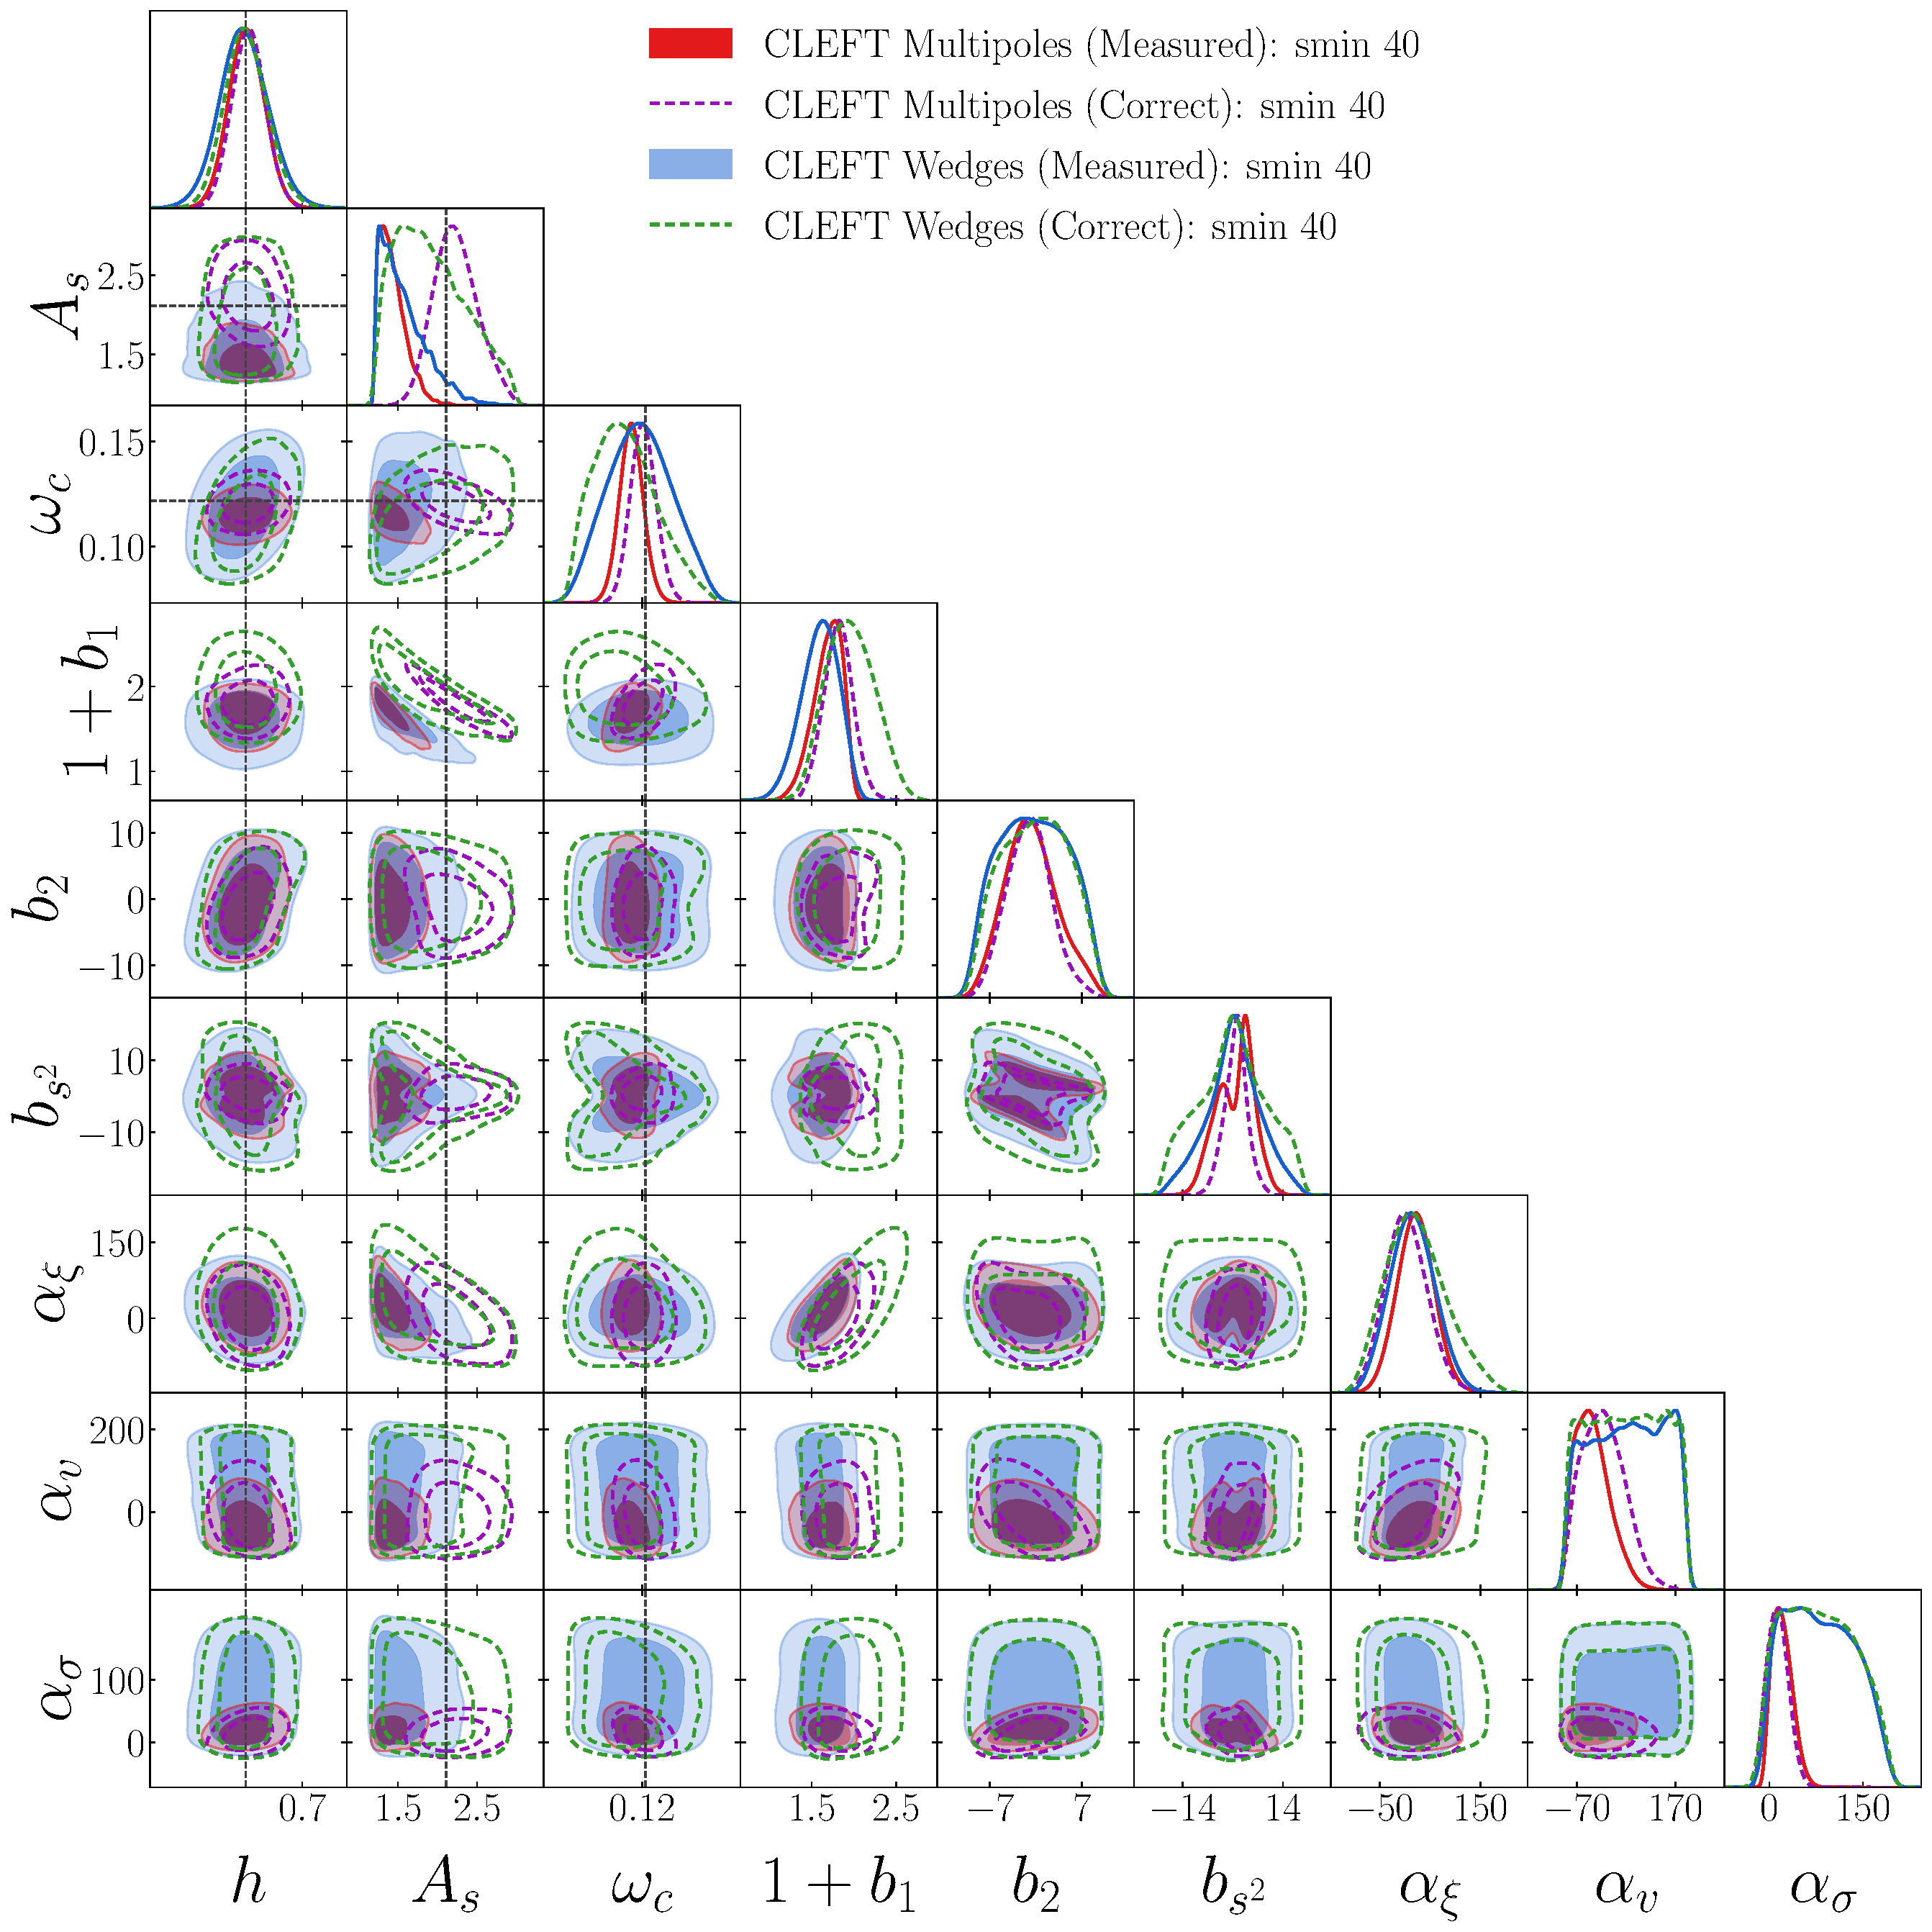
\includegraphics[width=\linewidth]{../graphs/z2_rebin/ELM_contours_CLEFT_smin_40_MMWW_MCMC.pdf}
        \label{fig:CLEFT_smin40_z2}
    \end{minipage}
    \caption{Contour plots for CLEFT model with scale-cut $s_\mathrm{min}=40 \, h^{-1}\mathrm{Mpc}$ for the redshift bin $z \in [0.9,1.1]$ in the left slot and $z \in [1.1,1.3]$ in the right slot.}
    \label{fig:CLEFT_smin40_z1vsz2}
\end{figure}

\begin{figure}[!ht]
    \centering
    \begin{minipage}{0.47\textwidth}
        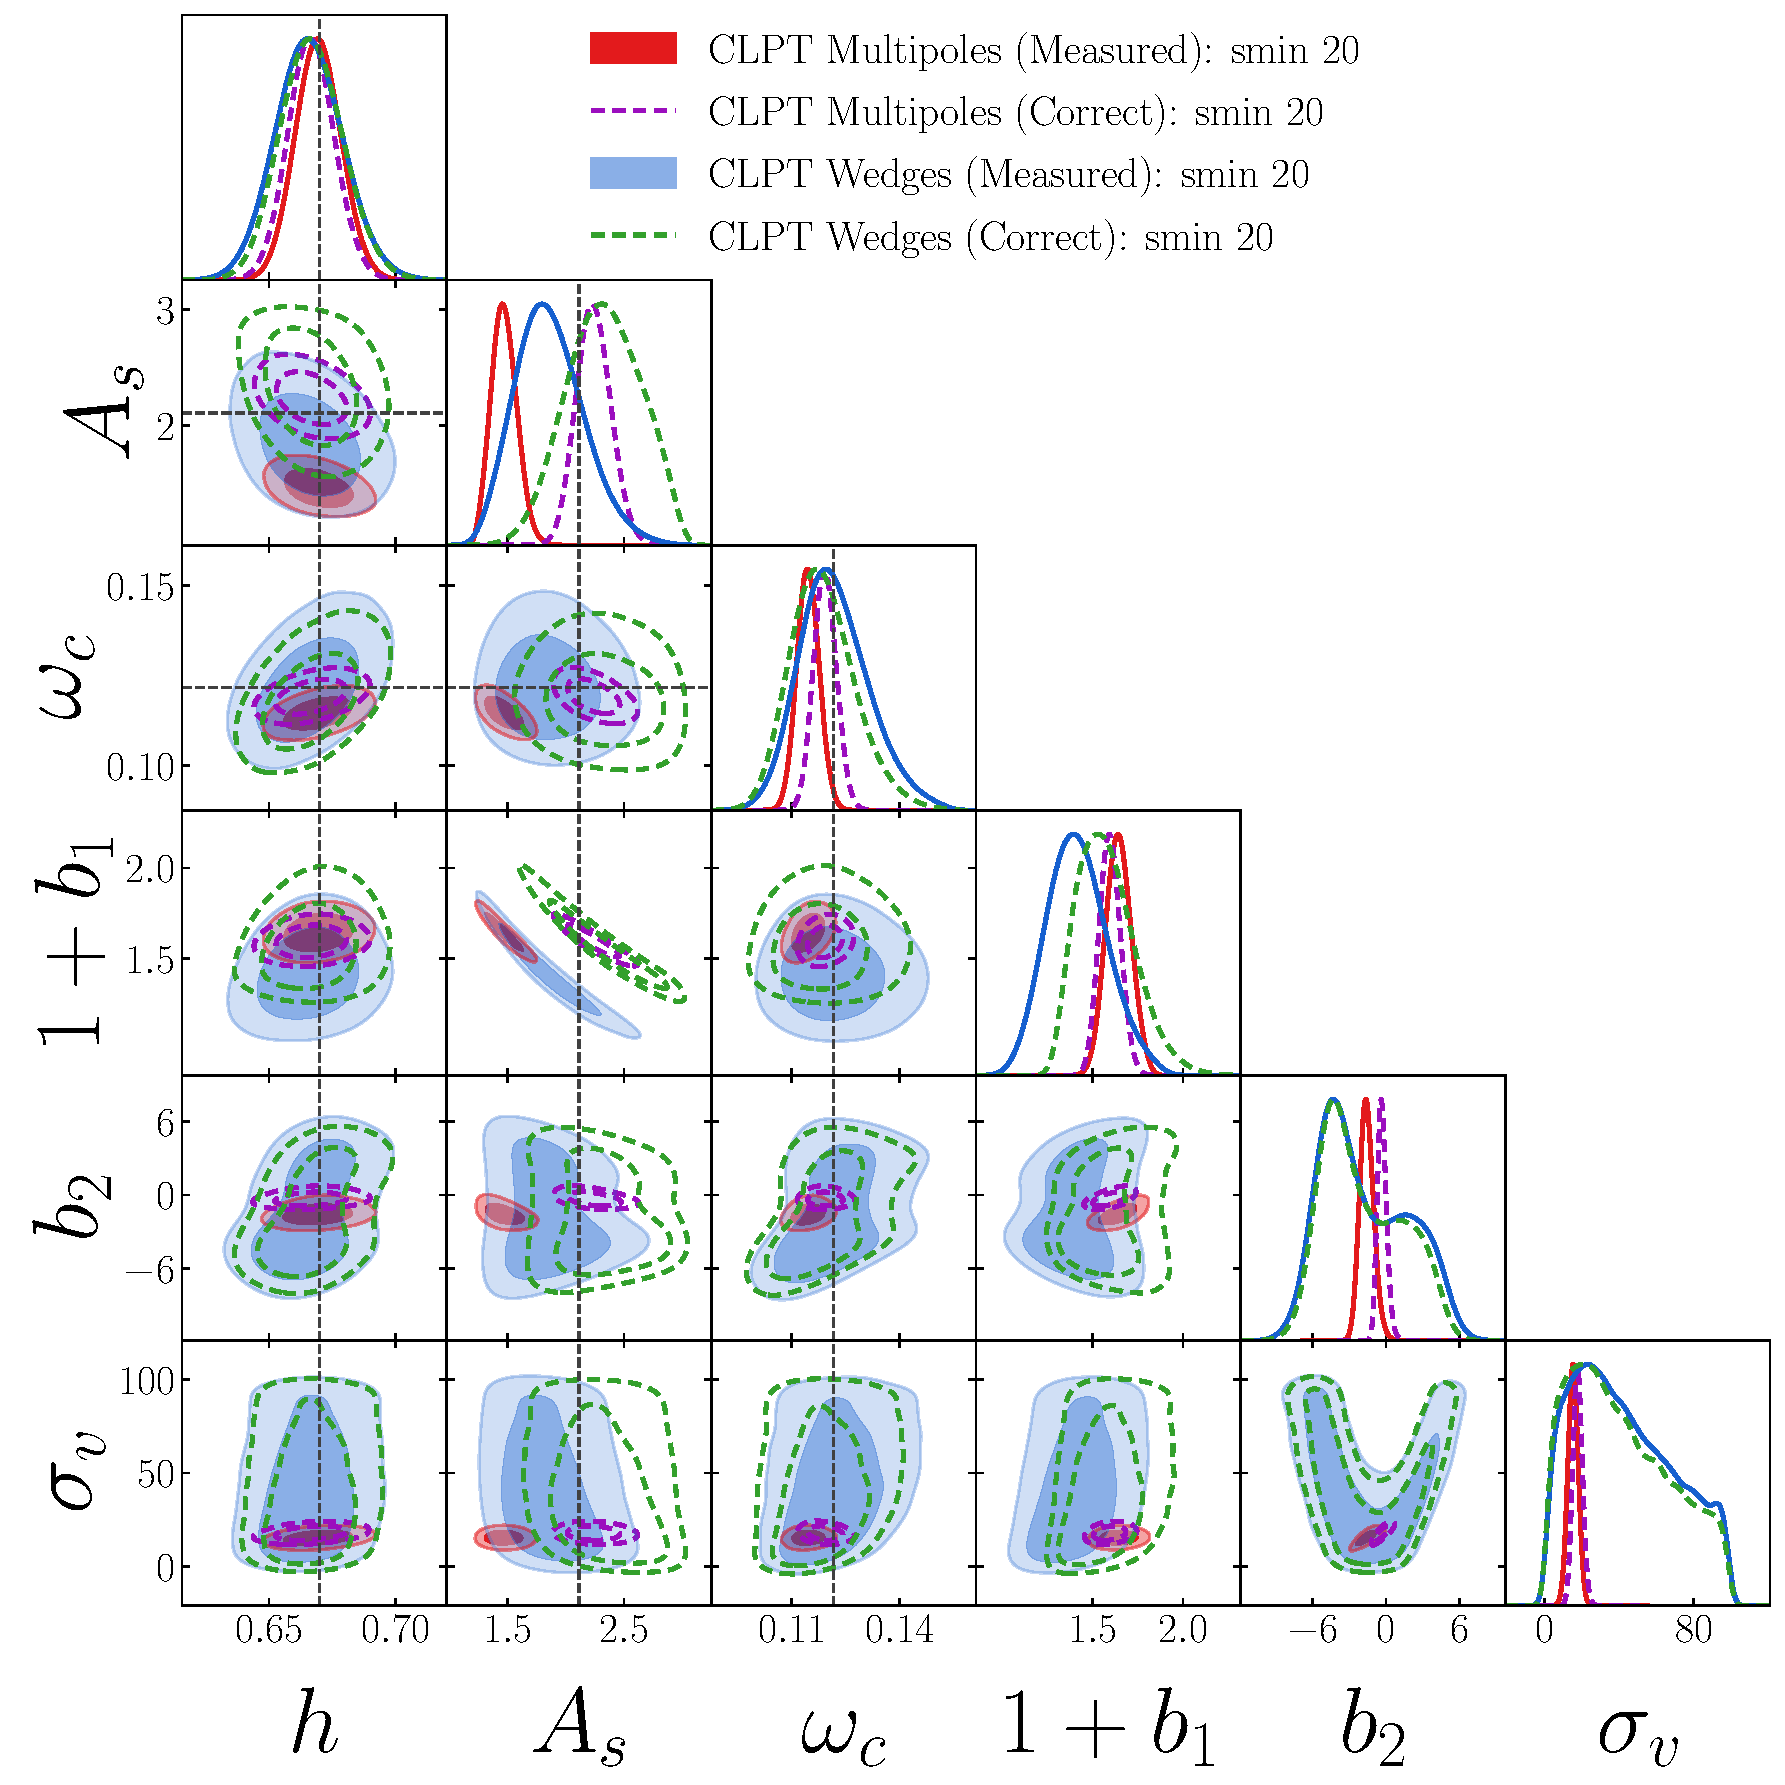
\includegraphics[width=\linewidth]{../graphs/z1_rebin/cluster/ELM_contours_CLPT_smin_20_MMWW_MCMC.pdf}
        \label{fig:CLPT_smin20_z1}
    \end{minipage}
    \hspace{0.5cm}
    \begin{minipage}{0.47\textwidth}
        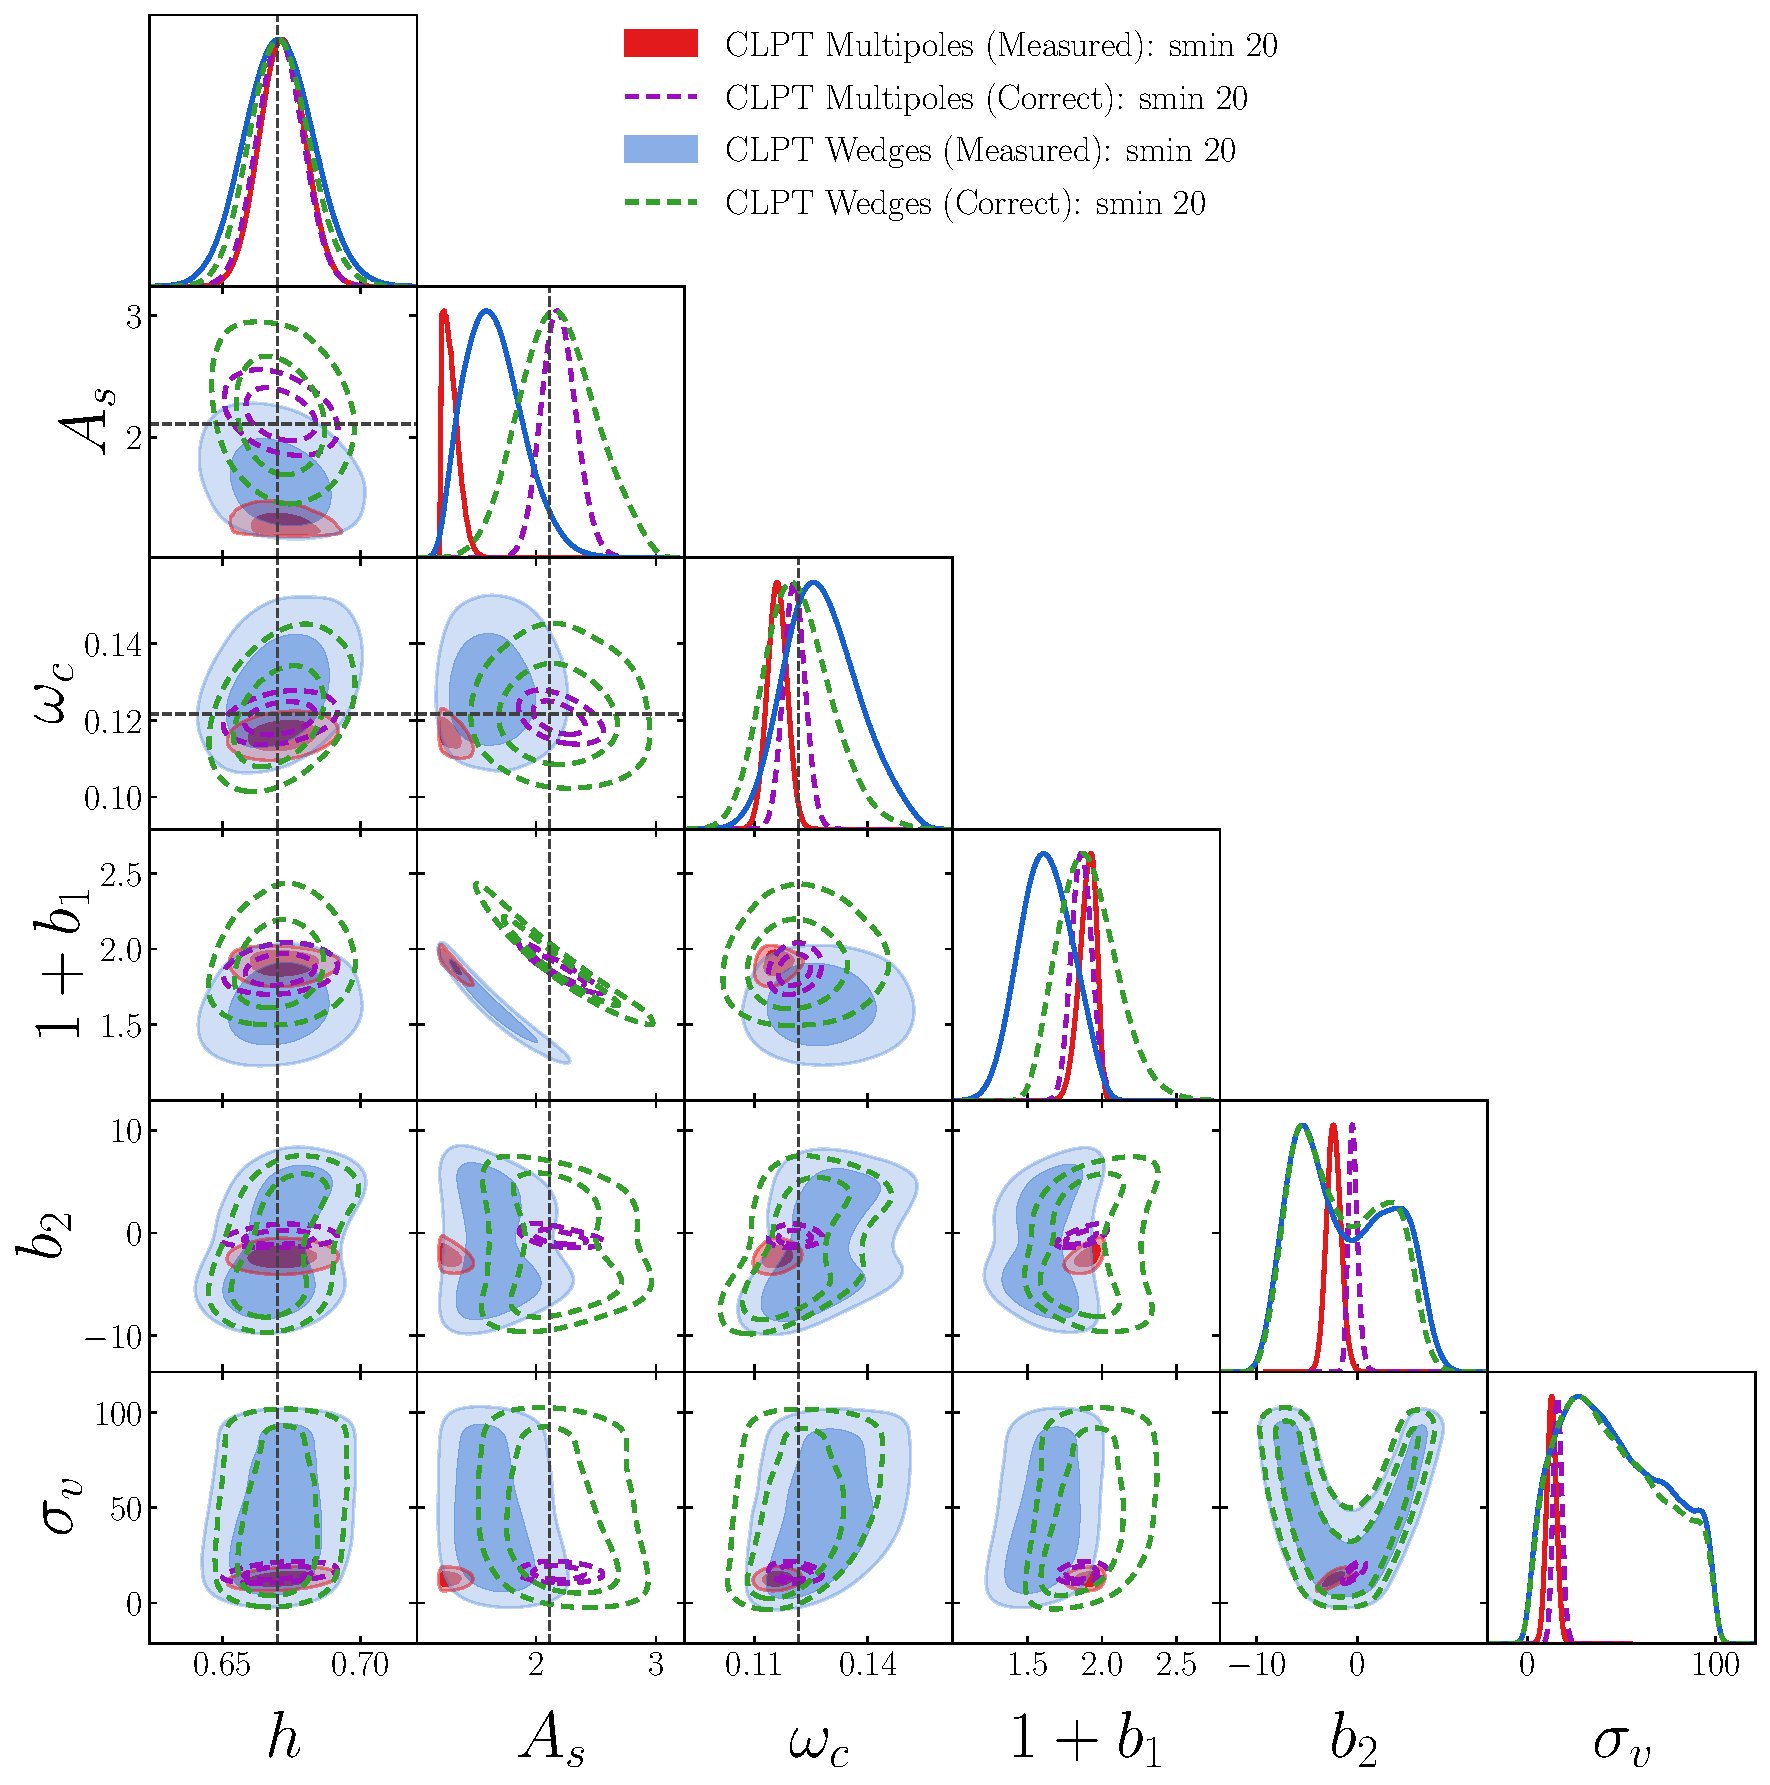
\includegraphics[width=\linewidth]{../graphs/z2_rebin/cluster/ELM_contours_CLPT_smin_20_MMWW_MCMC.pdf}
        \label{fig:CLPT_smin20_z2}
    \end{minipage}
    \caption{Contour plots for CLPT model with scale-cut $s_\mathrm{min}=20 \, h^{-1}\mathrm{Mpc}$ for the redshift bin $z \in [0.9,1.1]$ in the left slot and $z \in [1.1,1.3]$ in the right slot.}
    \label{fig:CLPT_smin20_z1vsz2}
\end{figure}
\begin{figure}[!ht]
    \centering
    \begin{minipage}{0.47\textwidth}
        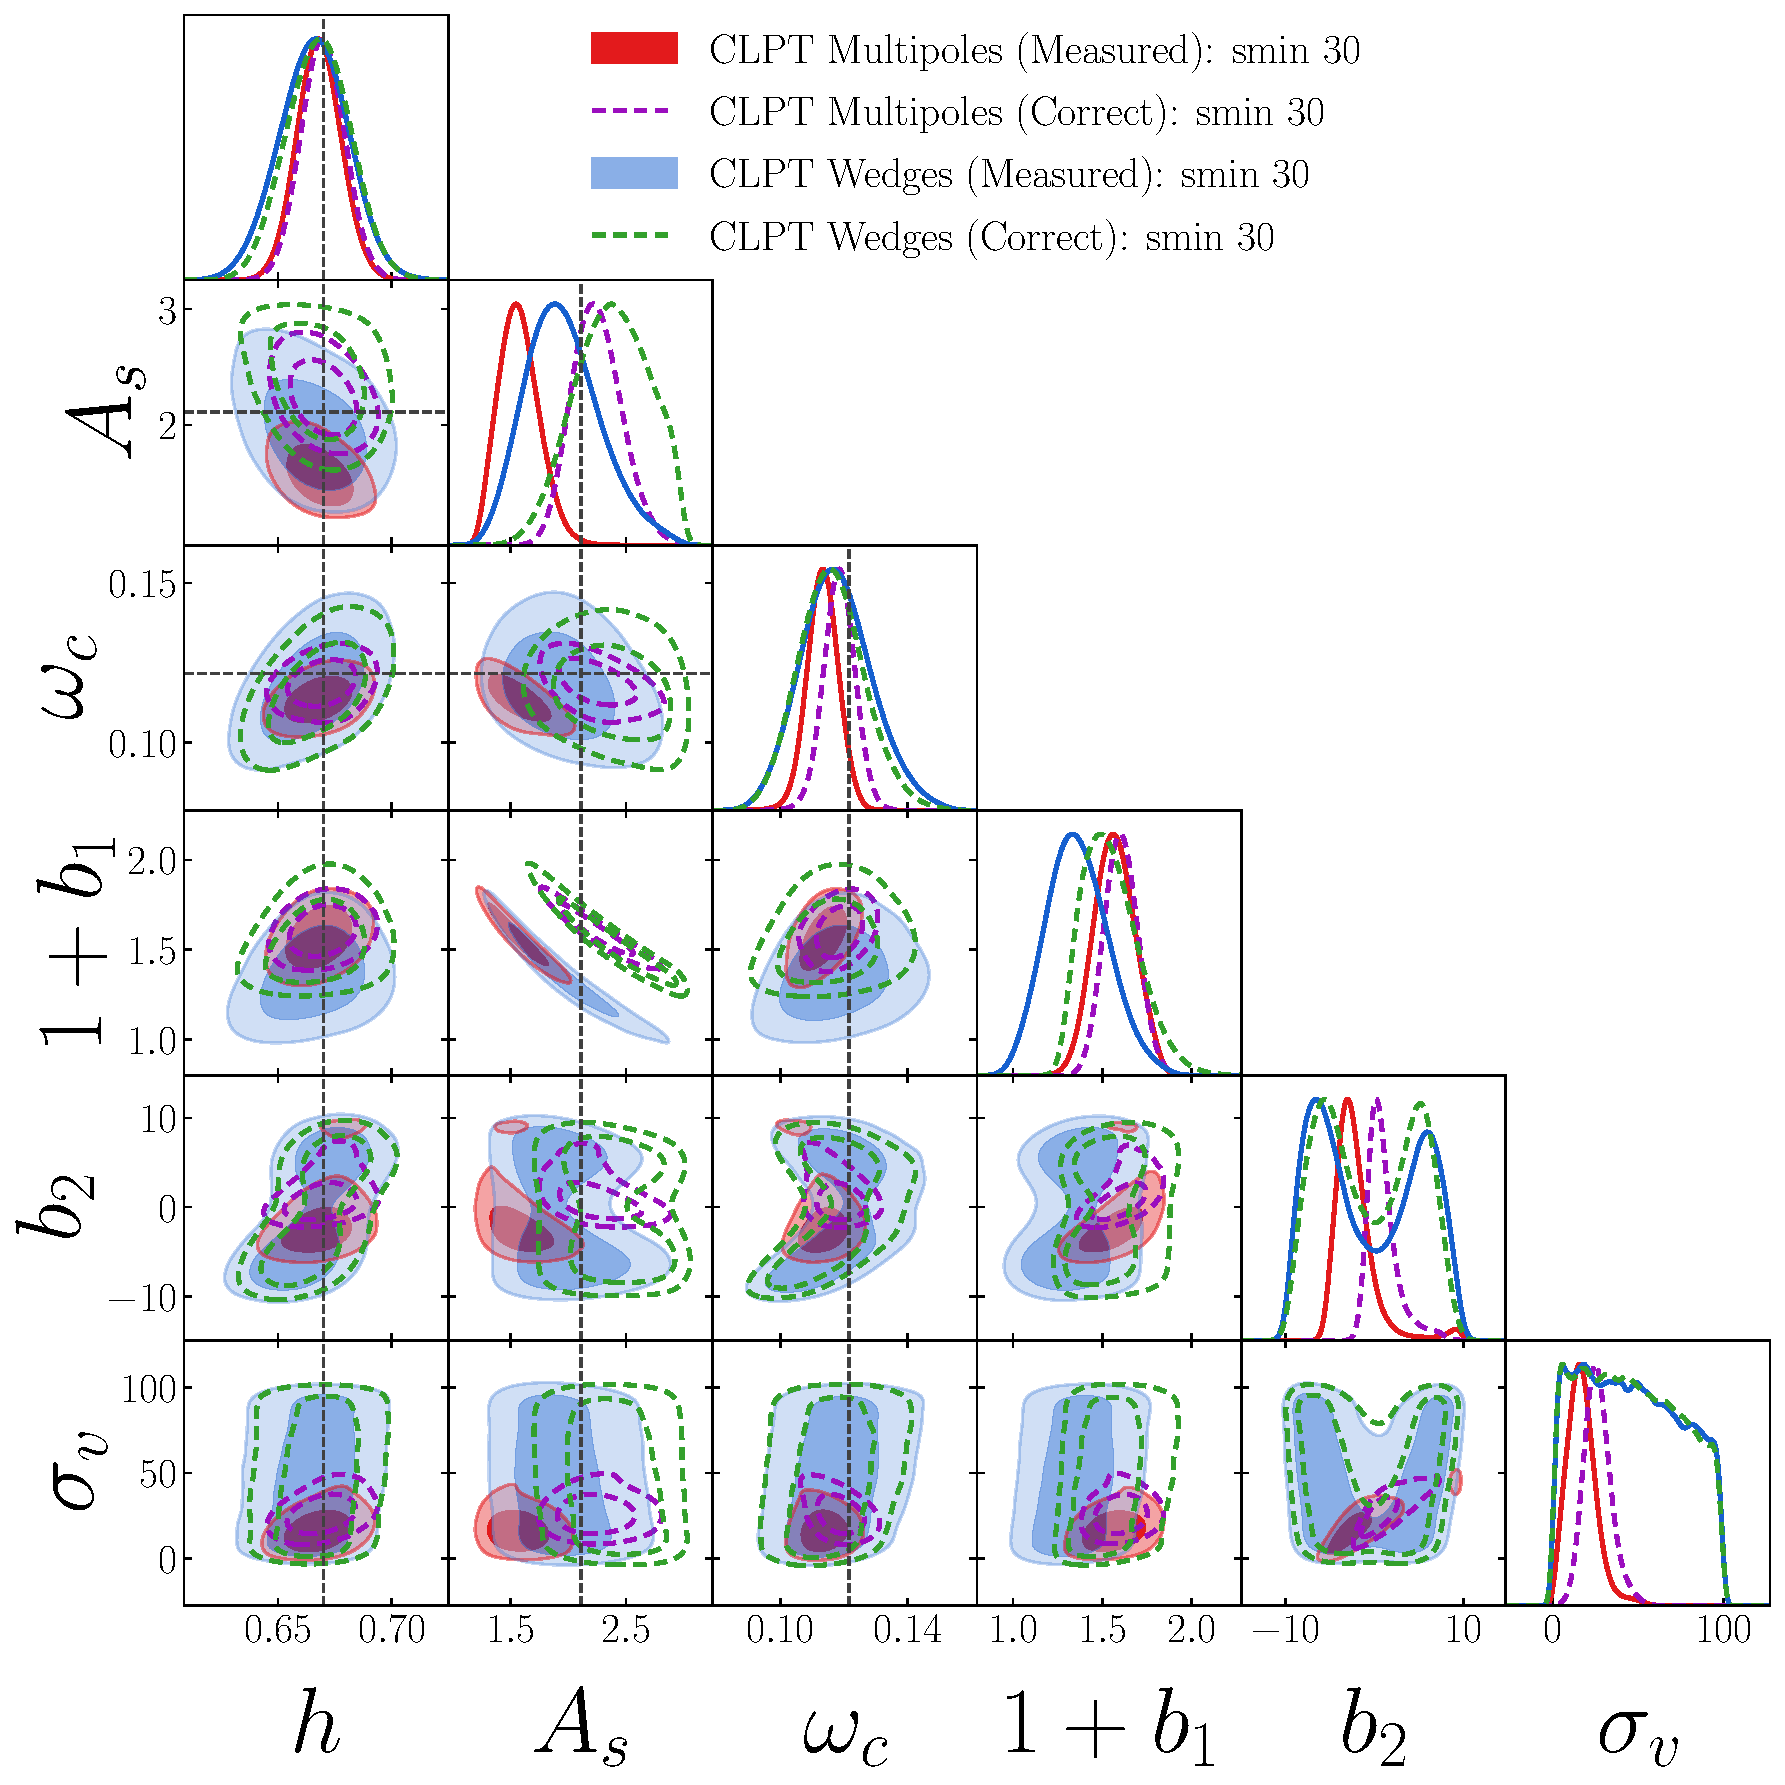
\includegraphics[width=\linewidth]{../graphs/z1_rebin/cluster/ELM_contours_CLPT_smin_30_MMWW_MCMC.pdf}
        \label{fig:CLPT_smin30_z1}
    \end{minipage}
    \hspace{0.5cm}
    \begin{minipage}{0.47\textwidth}
        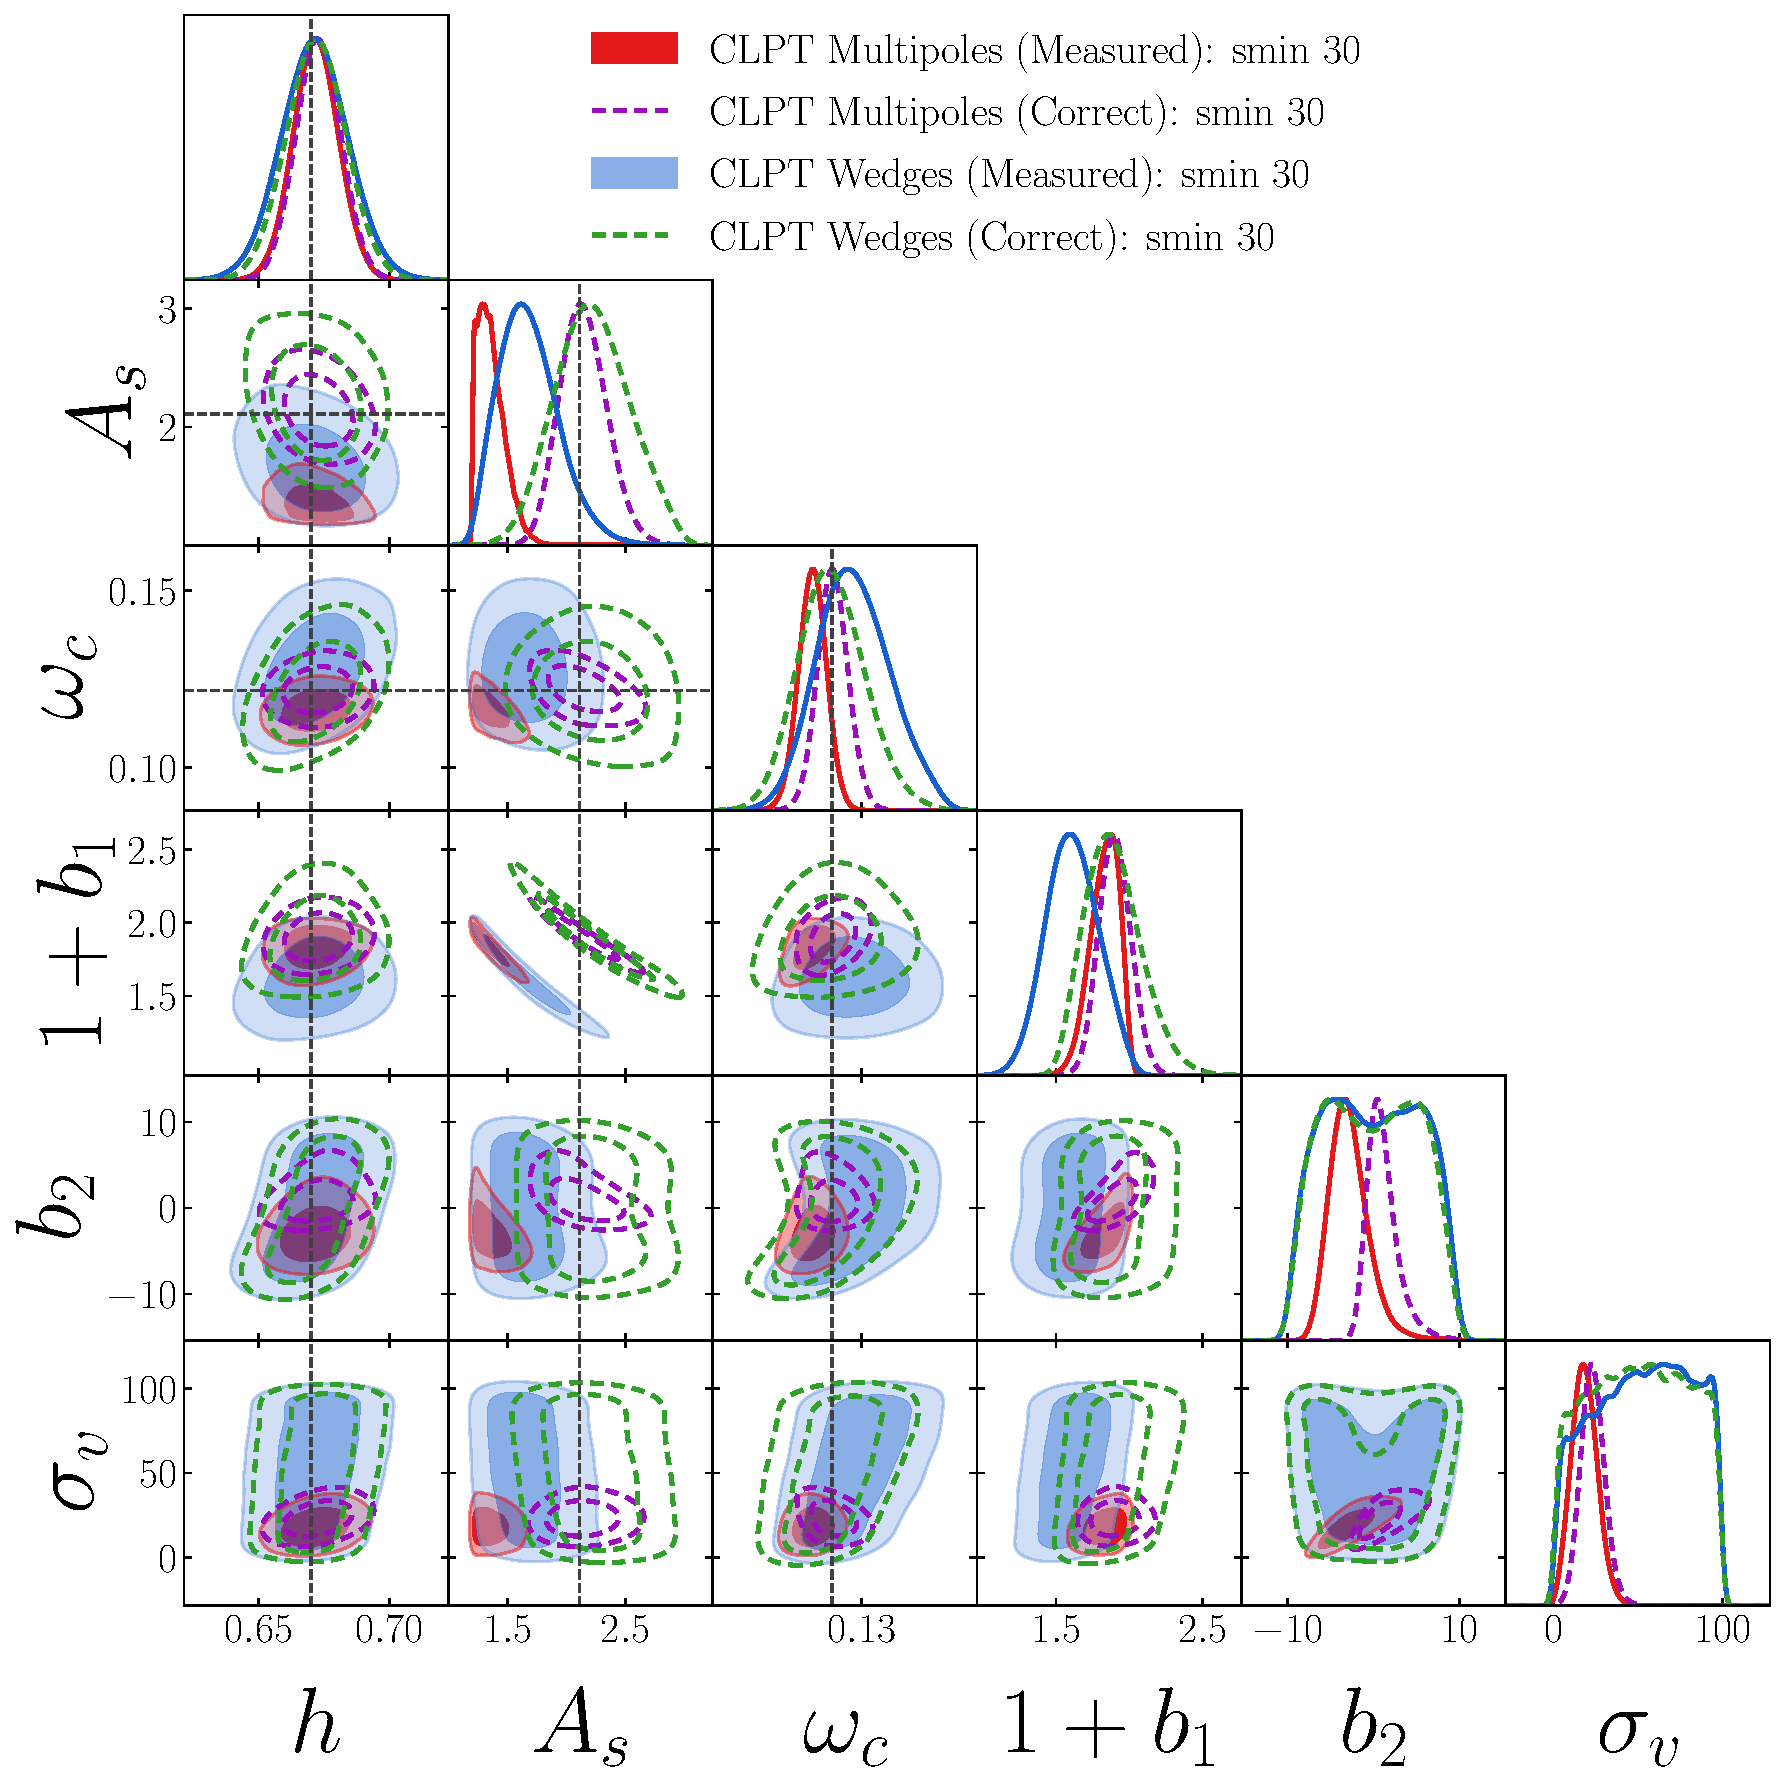
\includegraphics[width=\linewidth]{../graphs/z2_rebin/cluster/ELM_contours_CLPT_smin_30_MMWW_MCMC.pdf}
        \label{fig:CLPT_smin30_z2}
    \end{minipage}
    \caption{Contour plots for CLPT model with scale-cut $s_\mathrm{min}=30 \, h^{-1}\mathrm{Mpc}$ for the redshift bin $z \in [0.9,1.1]$ in the left slot and $z \in [1.1,1.3]$ in the right slot.}
    \label{fig:CLPT_smin30_z1vsz2}
\end{figure}

\subsection{Performance metrics}\label{subsec:PerformanceMetrics2}
Once the posterior distributions have been obtained, we can apply the performance metrics, presented in Sec.~\ref{sec:PerformanceMetrics}, in order to quantify and compare the ability of the two models to correctly estimate the cosmological parameters and to provide
accurate and precise constraints as a function of the scale-cut. The Fig.~\ref{fig:FoMFoB} shows a perfect summary of the relative performance of the models in a single plot.

\begin{figure}[!ht]
    \centering
    \begin{minipage}{0.47\textwidth}
        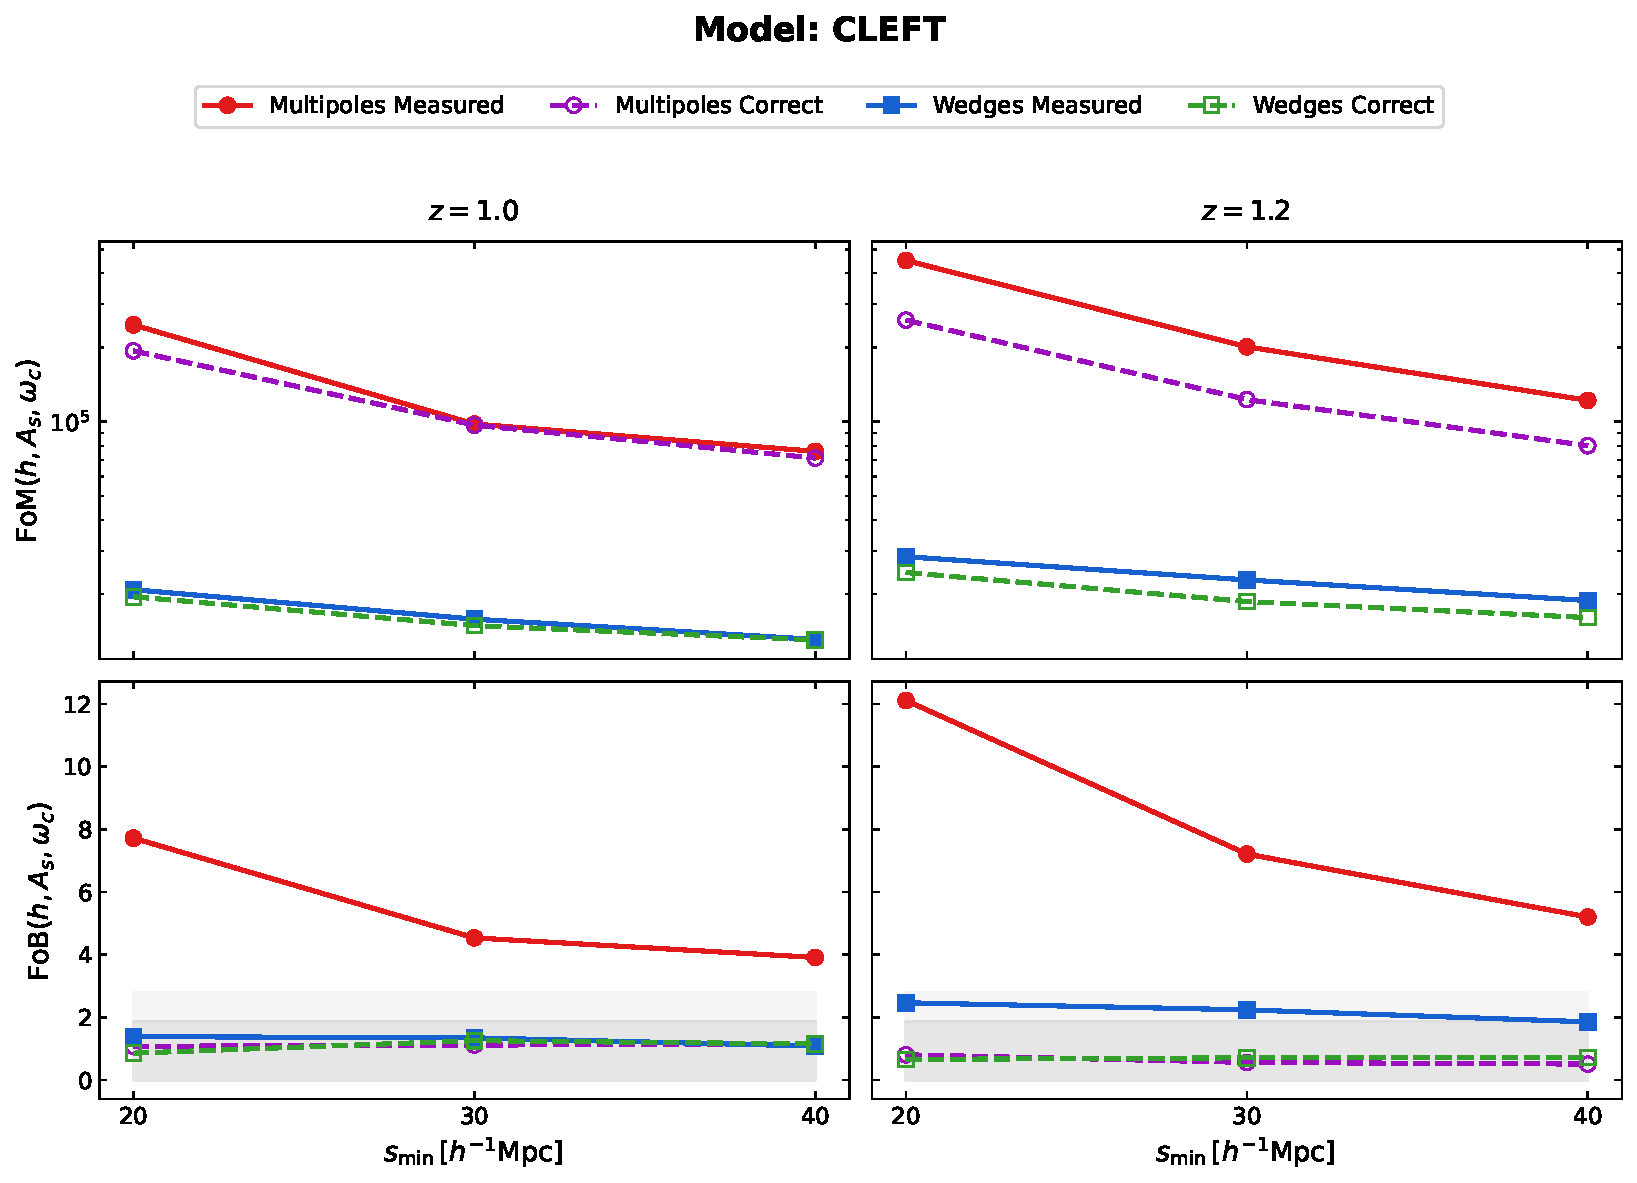
\includegraphics[width=\linewidth]{../graphs/z1_rebin/ELM_contours_CLEFT_FoM_FoB.pdf}
        \label{fig:CLEFT_FoMFoB}
    \end{minipage}
    \hspace{0.5cm}
    \begin{minipage}{0.47\textwidth}
        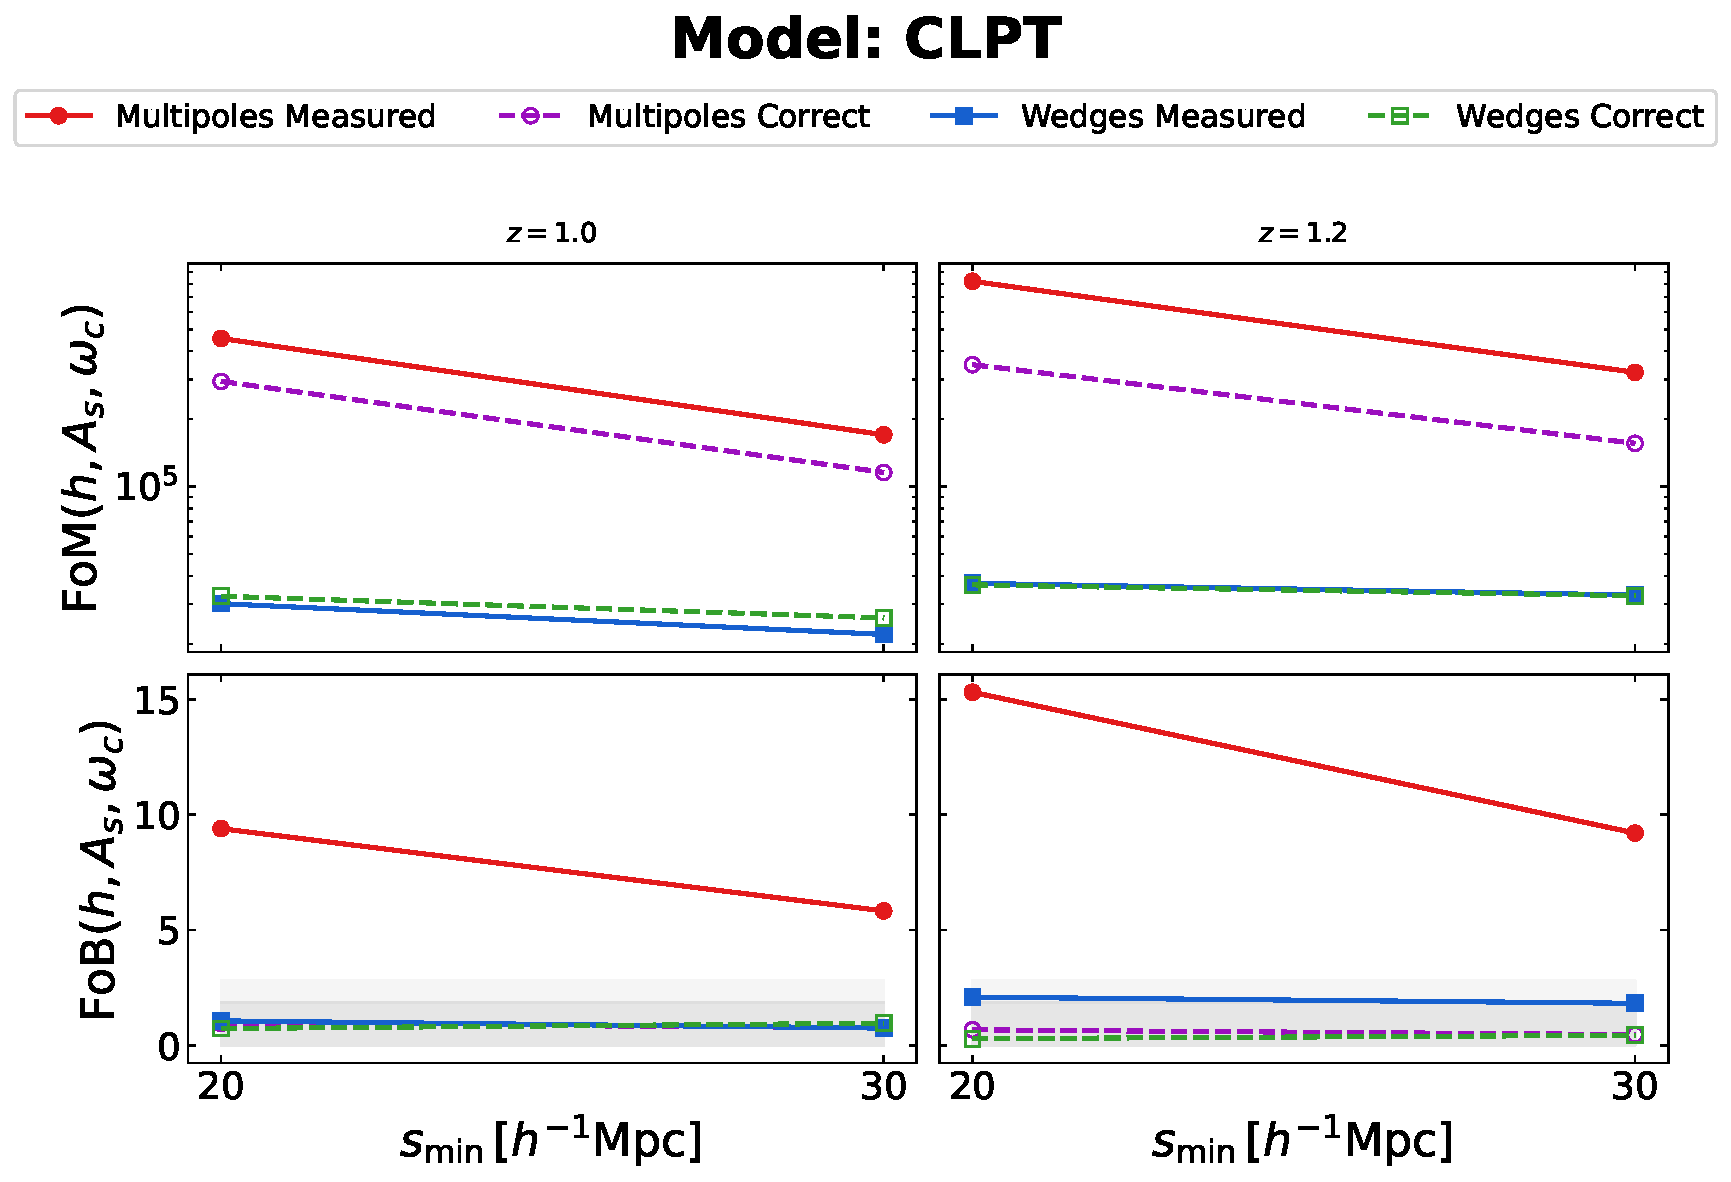
\includegraphics[width=\linewidth]{../graphs/z1_rebin/cluster/ELM_contours_CLPT_FoM_FoB.pdf}
        \label{fig:CLPT_FoMFoB}
    \end{minipage}
    \caption{FoB and FoM values for the fits obtained using the CLEFT and CLPT models for each redshift and as the scale-cut varies. The $\SI{68}{\percent}$ and $\SI{95}{\percent}$ regions are highlighted in dark gray and light gray, respectively.}
    \label{fig:FoMFoB}
\end{figure}

The top graphs show that the multipole method produces a FoM that is almost an order of magnitude higher than that of the wedge method. Even so, the bottom graphs reveal that this precision achieved with multipoles is biased: with the multipole expansion, the parameters are estimated with considerable precision but around a value far from the fiducial one. This is, most likely, due to the fact that contamination from interlopers in the line-of-sight spreads across all angular configurations during Legendre integration, corrupting every multipole. Therefore, the FoB clearly exceeds the acceptable region, shown in the picture as the dark grey region ($\SI{68}{\percent}$ confidence) and the light grey one ($\SI{95}{\percent}$ confidence).

On the other hand, the perpendicular wedge show significant stability against contamination from interlopers: for both models and for all redshifts, the FoB remains within the acceptable threshold, even on non-linear scales ($s_{min} = 20 \ h^{-1}\mathrm{Mpc}$), without losing too much in terms of precision.

\chapter{Conclusions}\label{chap:Conclusions}
In this thesis we have introduced and investigated the prominent systematic error in modern galaxy clustering pipelines: interloper contamination. The final goal of this work was to evaluate the impact of these errors onto cosmological parameter constraints.

Starting from realistic simulated data from EuclidLargeMocks, where we compare a clean dataset against a contaminated one, we adopted an analysis pipeline comparing two data compression strategies: standard Legendre multipoles and anisotropic clustering wedges. We then implemented Bayesian inference utilizing two non-linear structural modeling techniques, Convolution Lagrangian Perturbation Theory (CLPT) and Convolution Lagrangian Effective Field Theory (CLEFT), to extract the corresponding cosmological parameters. Finally, we evaluated the performance of these models using two primary metrics: the Figure of Bias and the Figure of Merit.

The analysis revealed that the introduction of interlopers into a catalogue causes an attenuation of the two-point correlation function. For this reason, the model misinterprets this interloper-induced signal attenuation as an intrinsically less clustered universe, ultimately underestimating the amplitude of the power spectrum $A_\mathrm{s}$. Simultaneously, distortions and damping of the BAO peak cause variations in the cold dark matter density $\omega_\mathrm{c}$.

By quantifying these results through FoM and Fob, we have revealed that, as the minimum fitting scale $s_\mathrm{min}$ is pushed deeper into the non-linear regime, the multipoles FoM increases by nearly an order of magnitude, while simultaneously pushing FoB well past the acceptable region of $\SI{68}{\percent}$ confidence. On the other hand, our analysis of the ratios revealed that the transverse wedge undergoes a particularly flat suppression. As a result, the perpendicular wedge manages to keep the FoB within the acceptable region (with a $\SI{68}{\percent}$ confidence level), but at the cost of a lower FoM.

\bibliographystyle{IEEEtran}
\bibliography{bibliography}

\end{document}